\documentclass[12pt,a4paper]{scrreprt}

% Essential packages
\usepackage[utf8]{inputenc}     % Input encoding
\usepackage[T1]{fontenc}        % Font encoding
\usepackage{graphicx}           % For images
\usepackage{wrapfig}            % to place figures on the side of text
\usepackage{amsmath,amssymb}    % For math equations
\usepackage{booktabs}           % For professional tables
\usepackage{listings}           % For code listings
\usepackage{setspace}           % For line spacing
\usepackage[margin=2.5cm, top=1.5cm, includehead, headheight=14pt, headsep=10pt]{geometry} % Page margins
%\usepackage{titlesec}           % For customizing section titles            
\usepackage[numbers,sort&compress]{natbib} % For references in bib format
\usepackage{xcolor}             % make it pretty
\usepackage{float}              % needed for placing images where you want them
\usepackage{caption}
\usepackage{pgf}
\usepackage[hyphens]{url}       % break URLs with hyphen in Bibliography
\usepackage{enumitem}           % enumerate ie. numbered bullet points
% Comment out the darkmode line for final PDF
%\usepackage{xcolor} \pagecolor[rgb]{0,0,0} \color[rgb]{1,1,1} % DARKMODE PDF 

\usepackage{chngcntr}
\counterwithout{equation}{chapter}


% TikZ packages for flowchart
\usepackage{tikz}
\usetikzlibrary{shapes.geometric, arrows, positioning, fit, backgrounds}
\usepackage[hidelinks]{hyperref}% For clickable links in PDF

% Define styles for TikZ
\tikzset{
  block/.style = {rectangle, draw, fill=blue!20, 
                  text width=8em, text centered, rounded corners, minimum height=2em},
  line/.style = {draw, -latex'},
  cloud/.style = {draw, ellipse, fill=red!20, minimum height=2em},
  group/.style = {draw, inner sep=0.3cm, rounded corners, fill=blue!5, label={#1}},
}

%%    ~~~  For list of Equations   ~~~
% use tocbasic package included with KOMA-Script
\DeclareNewTOC[
  type=equation,
  types=equations,
  name=Equation,
  listname=List of Equations
]{loe}
\setuptoc{loe}{numberwidth=23pt}
% command to add entries to the equation list:
\newcommand{\addequation}[1]{%
  \addxcontentsline{loe}{equation}{\protect\numberline{\theequation}#1}%
}



% Python code listing style
\definecolor{codegreen}{rgb}{0,0.6,0}
\definecolor{codegray}{rgb}{0.5,0.5,0.5}
\definecolor{codepurple}{rgb}{0.58,0,0.82}
\definecolor{backcolour}{rgb}{0.95,0.95,0.92}

\lstdefinestyle{pythonstyle}{
    backgroundcolor=\color{backcolour},   
    commentstyle=\color{codegreen},
    keywordstyle=\color{magenta},
    numberstyle=\tiny\color{codegray},
    stringstyle=\color{codepurple},
    basicstyle=\ttfamily\footnotesize,
    breakatwhitespace=false,         
    breaklines=true,                 
    captionpos=b,                    
    keepspaces=true,                 
    numbers=left,                    
    numbersep=5pt,                  
    showspaces=false,                
    showstringspaces=false,
    showtabs=false,                  
    tabsize=2,
    language=Python
}

% C code listing style
\definecolor{codegreen}{rgb}{0,0.6,0}
\definecolor{codegray}{rgb}{0.5,0.5,0.5}
\definecolor{codepurple}{rgb}{0.58,0,0.82}
\definecolor{backcolour}{rgb}{0.95,0.95,0.92}
\lstdefinestyle{cstyle}{
    backgroundcolor=\color{backcolour},   
    commentstyle=\color{codegreen},
    keywordstyle=\color{magenta},
    numberstyle=\tiny\color{codegray},
    stringstyle=\color{codepurple},
    basicstyle=\ttfamily\footnotesize,
    breakatwhitespace=false,         
    breaklines=true,                 
    captionpos=b,                    
    keepspaces=true,                 
    numbers=left,                    
    numbersep=5pt,                  
    showspaces=false,                
    showstringspaces=false,
    showtabs=false,                  
    tabsize=2,
    language=C
}



% Set the default style for listings
\lstset{style=pythonstyle}

% % Redifine the chapter format to remove Chapter 1 2 etc
% \titleformat{\chapter}[hang]
% {\normalfont\huge\bfseries}{\thechapter.}{1em}{}

% Include title page
% Define title page information
\title{
    {\LARGE\textbf{GLASGOW CALEDONIAN UNIVERSITY}} \\
    \vspace{1.5cm}
    {\LARGE MEng Group Research Project } \\
    \vspace{0.5cm}
    {\LARGE MMH723842-24-AB-GLAS} \\
    \vspace{1.5cm}
    {\LARGE\textbf{Design and implementation of a PSD-Based Analogue 2D Sun Sensor}} \\
    \vspace{0.5cm}
    {\large word count: xxx} \\
}

\author{
    by Zac McCaffery, Alexandru Belea,  \\
    Sebastian Alexander, William Kong, Nassor Salim,
}

\date{
    Date: \today
}


% Document begins
\begin{document}

% Set line spacing to 1.5
\onehalfspacing

% Create fancy title page
\begin{titlepage}
    \maketitle
    \thispagestyle{empty}
\end{titlepage}

% Table of contents page
\tableofcontents
\thispagestyle{empty}
\clearpage

% List of figures
\listoffigures
\thispagestyle{empty}

% List of Equations
\listofequations


\clearpage
% Include chapters
% Add your chapters here or inside the sub-files
% abstract.tex
\chapter*{Abstract}
add abstract here
\addcontentsline{toc}{chapter}{Abstract}
\chapter{Acknowledgements}


We would like to express our sincere gratitude to our supervisors, Dr. Roberto Ramirez-Iniguez and Geraint Bevan, for their invaluable guidance and unwavering support throughout this project.

Our appreciation extends to the 3rd Floor EEE Lab Technicians and Dr. Carlos Gamio-Roffe, whose technical expertise and assistance were instrumental in the successful construction of the prototype.

We are particularly grateful to the European Project Semester RED Team members—Nikolay Ivanov Shopov, Stef Hannisse, and Samridhi Gupta—for generously allowing the use of their Renewable Energy Demonstrator as a testbench. Their contribution provided an ideal platform for positioning light sources during the testing phase of this project.
% introduction.tex
\chapter{Introduction}
% Your introduction content here
Write intro here \cite{rosebrock2019label}
\chapter{Literature Review}
% add subsections
% Methodology.tex
\chapter{Methodology}

% Include each section from separate files
% SystemDesignOverview.tex
\section{System Design Overview}
This section provides an overview of the System Design Overview.

% Include a flowchart
\begin{figure}[H]
    \centering
    \scalebox{0.8}{ % Scale to 80% of original size
        % try generating flowcharts as svg in Claude 
% and edit with inkscape instead of this.
% but claude did generate this one so might 
% be useful too but you can't easily make
% small repairs in inkscape


% CNN Transfer Learning Flowchart - Compact Multi-Column Layout
% \begin{figure}[htbp]

\centering
\resizebox{\textwidth}{!}{ % Scale to fit width while maintaining aspect ratio
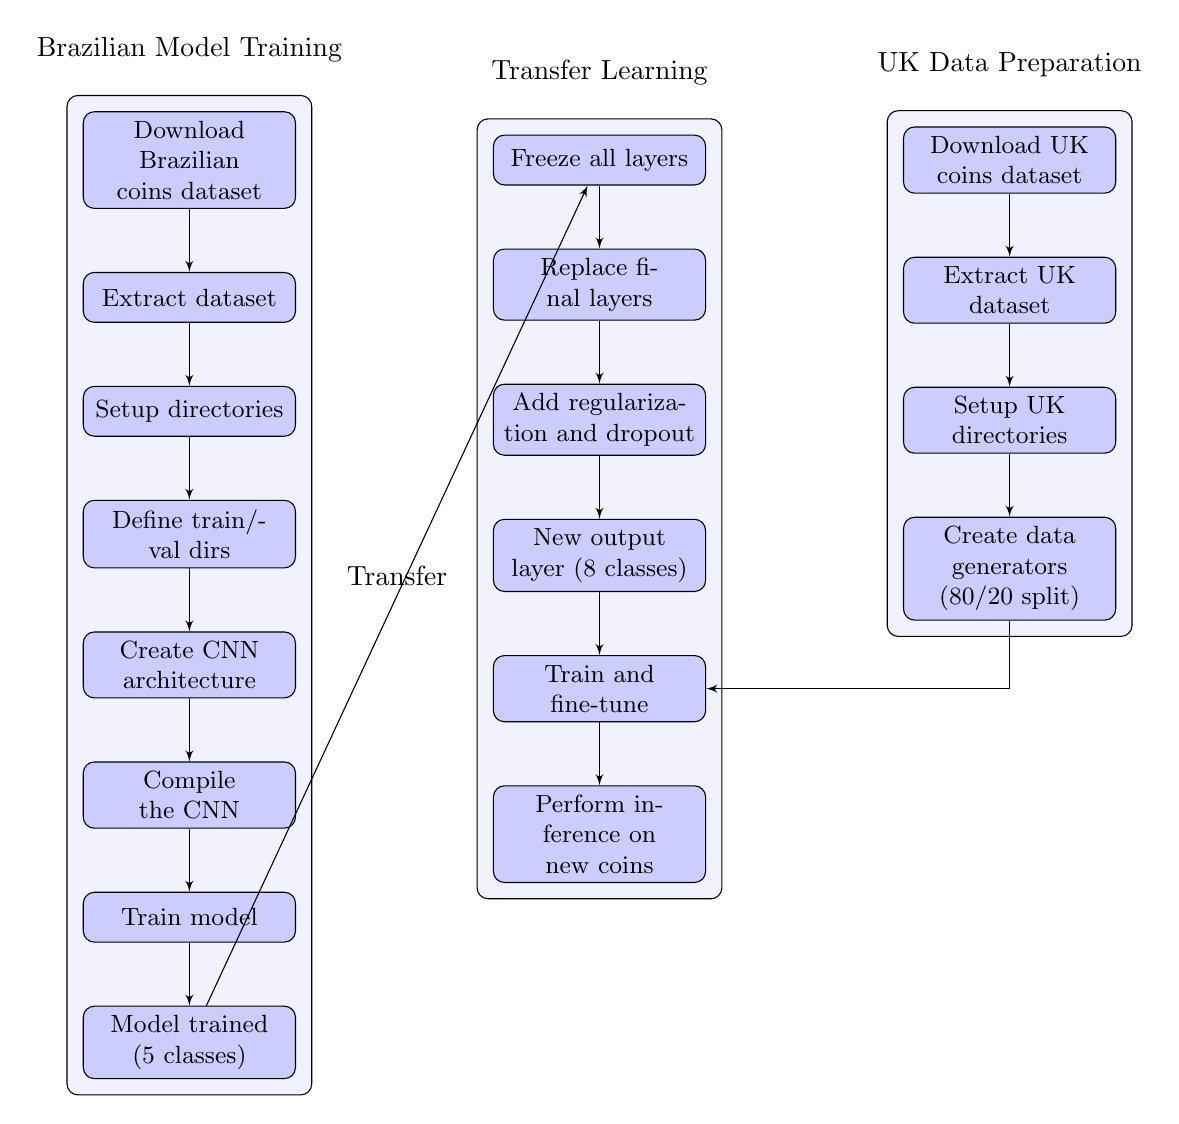
\begin{tikzpicture}[node distance=0.8cm and 1.5cm, auto]
    % Define a smaller block style
    \tikzset{
      block/.style = {rectangle, draw, fill=blue!20, 
                      text width=7em, text centered, rounded corners, minimum height=1.8em, font=\small},
    }
    
    % Brazilian model training - Column 1
    \node [block] (brazildata) {Download Brazilian coins dataset};
    \node [block, below=of brazildata] (extract) {Extract dataset};
    \node [block, below=of extract] (setup) {Setup directories};
    \node [block, below=of setup] (define) {Define train/val dirs};
    \node [block, below=of define] (create) {Create CNN architecture};
    \node [block, below=of create] (compile) {Compile the CNN};
    \node [block, below=of compile] (train) {Train model};
    \node [block, below=of train] (trained) {Model trained (5 classes)};
    
    % Transfer learning - Column 2 (Middle)
    \node [block, right=2.5cm of brazildata] (freeze) {Freeze all layers};
    \node [block, below=of freeze] (replace) {Replace final layers};
    \node [block, below=of replace] (add) {Add regularization and dropout};
    \node [block, below=of add] (output) {New output layer (8 classes)};
    \node [block, below=of output] (finaltrain) {Train and fine-tune};
    \node [block, below=of finaltrain] (inference) {Perform inference on new coins};
    
    % UK data preparation - Column 3 (Right)
    \node [block, right=2.5cm of freeze] (ukdata) {Download UK coins dataset};
    \node [block, below=of ukdata] (ukextract) {Extract UK dataset};
    \node [block, below=of ukextract] (uksetup) {Setup UK directories};
    \node [block, below=of uksetup] (ukgen) {Create data generators (80/20 split)};
    
    % Connect all nodes with arrows
    \path [line] (brazildata) -- (extract);
    \path [line] (extract) -- (setup);
    \path [line] (setup) -- (define);
    \path [line] (define) -- (create);
    \path [line] (create) -- (compile);
    \path [line] (compile) -- (train);
    \path [line] (train) -- (trained);
    
    \path [line] (ukdata) -- (ukextract);
    \path [line] (ukextract) -- (uksetup);
    \path [line] (uksetup) -- (ukgen);
    
    % Connect the columns
    \path [line] (trained) -- node[midway, above] {Transfer} (freeze);
    \path [line] (ukgen) |- (finaltrain);
    
    % Connect middle column
    \path [line] (freeze) -- (replace);
    \path [line] (replace) -- (add);
    \path [line] (add) -- (output);
    \path [line] (output) -- (finaltrain);
    \path [line] (finaltrain) -- (inference);
    
    % Group boxes to show different stages with smaller padding
    \begin{pgfonlayer}{background}
        \node[group={[yshift=0.3cm]above:Brazilian Model Training}, fit={(brazildata) (extract) (setup) (define) (create) (compile) (train) (trained)}, inner sep=0.2cm] {};
        \node[group={[yshift=0.3cm]above:UK Data Preparation}, fit={(ukdata) (ukextract) (uksetup) (ukgen)}, inner sep=0.2cm] {};
        \node[group={[yshift=0.3cm]above:Transfer Learning}, fit={(freeze) (replace) (add) (output) (finaltrain) (inference)}, inner sep=0.2cm] {};
    \end{pgfonlayer}
\end{tikzpicture}
}
% \caption{CNN Transfer Learning Flowchart: Brazilian to UK Coins}
% \label{fig:cnn-flowchart}
% \end{figure}
    }
    \caption{System Design Overview Flowchart}
    \label{fig:decriptiveLabel77} % descriptive to call in text with \ref{fig:decriptiveLabel77}
\end{figure}

\subsection{Functional Requirements}
% Your content here

\subsection{Design Approach}
% Your content here

\subsection{System Architecture}
As shown in Figure~\ref{fig:decriptiveLabel77} the system architecture consists of various components.

\begin{lstlisting}[style=cstyle, caption=System Architecture Code Example, label=lst:SystemArchitecture13]
# Your code here
\end{lstlisting}

\begin{figure}[htbp] %h-ere t-op b-ottom p-page (separte) -good to allow all htbp to give the compiler more options
    \centering
    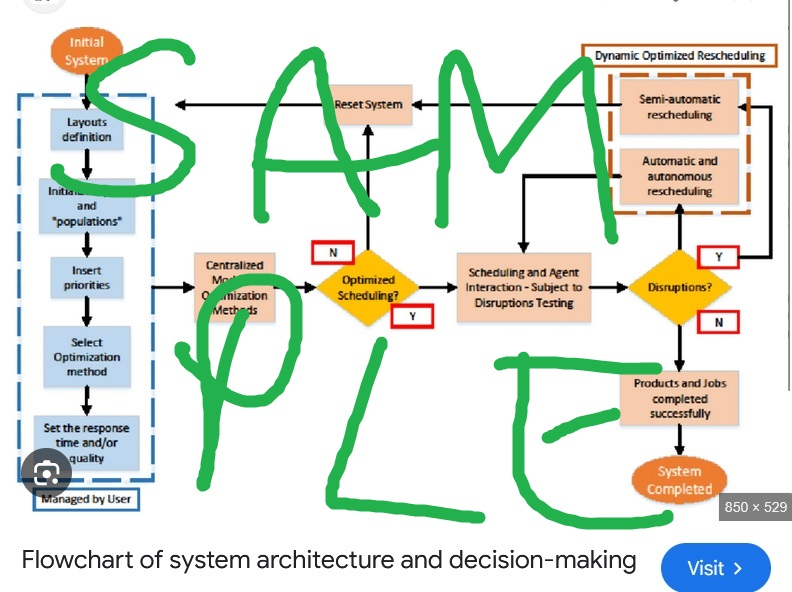
\includegraphics[width=0.6\textwidth]{figures/methodology/system_architecture.jpg}
    \caption{System Architecture Diagram}
    \label{fig:system-architecture1}
\end{figure}
% SensorArrayDevelopment.tex
\section{Sensor Array Development}
This section provides an overview of the Sensor Array Development.

% Include a flowchart
\begin{figure}[H]
    \centering
    \scalebox{0.8}{ % Scale to 80% of original size
        % try generating flowcharts as svg in Claude 
% and edit with inkscape instead of this.
% but claude did generate this one so might 
% be useful too but you can't easily make
% small repairs in inkscape


% CNN Transfer Learning Flowchart - Compact Multi-Column Layout
% \begin{figure}[htbp]

\centering
\resizebox{\textwidth}{!}{ % Scale to fit width while maintaining aspect ratio
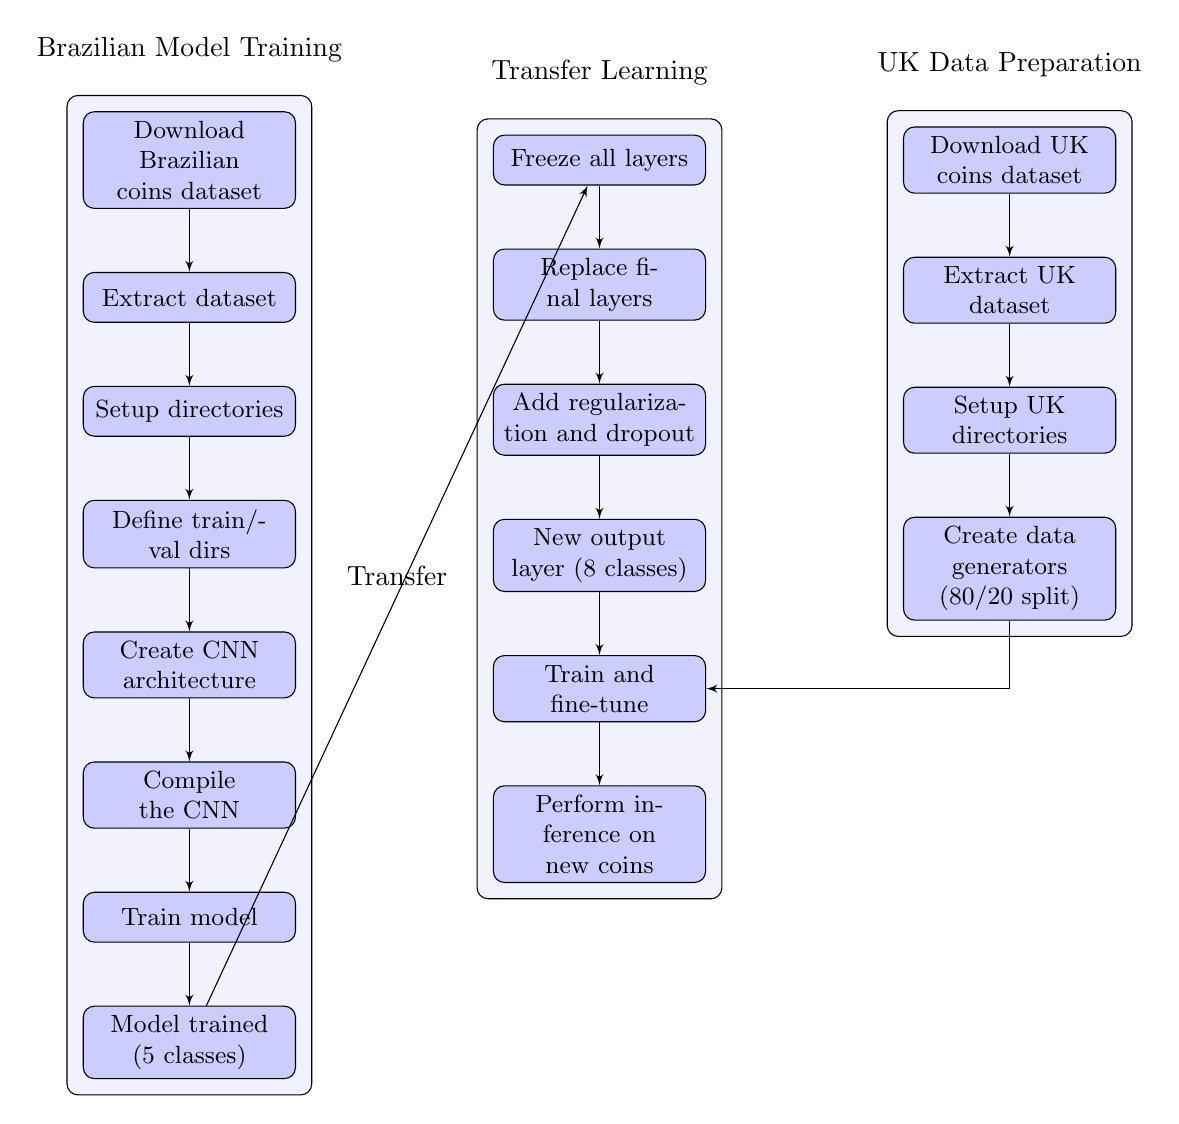
\begin{tikzpicture}[node distance=0.8cm and 1.5cm, auto]
    % Define a smaller block style
    \tikzset{
      block/.style = {rectangle, draw, fill=blue!20, 
                      text width=7em, text centered, rounded corners, minimum height=1.8em, font=\small},
    }
    
    % Brazilian model training - Column 1
    \node [block] (brazildata) {Download Brazilian coins dataset};
    \node [block, below=of brazildata] (extract) {Extract dataset};
    \node [block, below=of extract] (setup) {Setup directories};
    \node [block, below=of setup] (define) {Define train/val dirs};
    \node [block, below=of define] (create) {Create CNN architecture};
    \node [block, below=of create] (compile) {Compile the CNN};
    \node [block, below=of compile] (train) {Train model};
    \node [block, below=of train] (trained) {Model trained (5 classes)};
    
    % Transfer learning - Column 2 (Middle)
    \node [block, right=2.5cm of brazildata] (freeze) {Freeze all layers};
    \node [block, below=of freeze] (replace) {Replace final layers};
    \node [block, below=of replace] (add) {Add regularization and dropout};
    \node [block, below=of add] (output) {New output layer (8 classes)};
    \node [block, below=of output] (finaltrain) {Train and fine-tune};
    \node [block, below=of finaltrain] (inference) {Perform inference on new coins};
    
    % UK data preparation - Column 3 (Right)
    \node [block, right=2.5cm of freeze] (ukdata) {Download UK coins dataset};
    \node [block, below=of ukdata] (ukextract) {Extract UK dataset};
    \node [block, below=of ukextract] (uksetup) {Setup UK directories};
    \node [block, below=of uksetup] (ukgen) {Create data generators (80/20 split)};
    
    % Connect all nodes with arrows
    \path [line] (brazildata) -- (extract);
    \path [line] (extract) -- (setup);
    \path [line] (setup) -- (define);
    \path [line] (define) -- (create);
    \path [line] (create) -- (compile);
    \path [line] (compile) -- (train);
    \path [line] (train) -- (trained);
    
    \path [line] (ukdata) -- (ukextract);
    \path [line] (ukextract) -- (uksetup);
    \path [line] (uksetup) -- (ukgen);
    
    % Connect the columns
    \path [line] (trained) -- node[midway, above] {Transfer} (freeze);
    \path [line] (ukgen) |- (finaltrain);
    
    % Connect middle column
    \path [line] (freeze) -- (replace);
    \path [line] (replace) -- (add);
    \path [line] (add) -- (output);
    \path [line] (output) -- (finaltrain);
    \path [line] (finaltrain) -- (inference);
    
    % Group boxes to show different stages with smaller padding
    \begin{pgfonlayer}{background}
        \node[group={[yshift=0.3cm]above:Brazilian Model Training}, fit={(brazildata) (extract) (setup) (define) (create) (compile) (train) (trained)}, inner sep=0.2cm] {};
        \node[group={[yshift=0.3cm]above:UK Data Preparation}, fit={(ukdata) (ukextract) (uksetup) (ukgen)}, inner sep=0.2cm] {};
        \node[group={[yshift=0.3cm]above:Transfer Learning}, fit={(freeze) (replace) (add) (output) (finaltrain) (inference)}, inner sep=0.2cm] {};
    \end{pgfonlayer}
\end{tikzpicture}
}
% \caption{CNN Transfer Learning Flowchart: Brazilian to UK Coins}
% \label{fig:cnn-flowchart}
% \end{figure}
    }
    \caption{System Design Overview Flowchart}
    \label{fig:decriptiveLabel55} % descriptive to call in text with \ref{fig:decriptiveLabel55}
\end{figure}

\subsection{Functional Requirements}
% Your content here

\subsection{Design Approach}
% Your content here

\subsection{System Architecture}
As shown in Figure~\ref{fig:decriptiveLabel55} the system architecture consists of various components.

\begin{lstlisting}[style=cstyle, caption=System Architecture Code Example, label=lst:SystemArchitecture11]
# Your code here
\end{lstlisting}

\begin{figure}[htbp] %h-ere t-op b-ottom p-page (separte) -good to allow all htbp to give the compiler more options
    \centering
    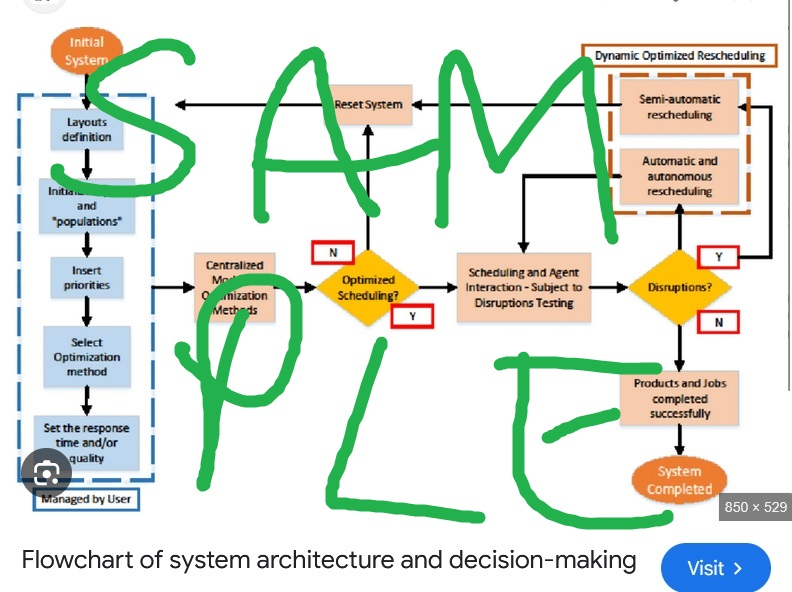
\includegraphics[width=0.6\textwidth]{figures/methodology/system_architecture.jpg}
    \caption{System Architecture Diagram}
    \label{fig:system-architecture6}
\end{figure}
% SignalConditioningCircuitry.tex
\section{Signal Conditioning Circuitry}
This section provides an overview of the Signal Conditioning Circuitry.

% Include a flowchart
\begin{figure}[H]
    \centering
    \scalebox{0.8}{ % Scale to 80% of original size
        % try generating flowcharts as svg in Claude 
% and edit with inkscape instead of this.
% but claude did generate this one so might 
% be useful too but you can't easily make
% small repairs in inkscape


% CNN Transfer Learning Flowchart - Compact Multi-Column Layout
% \begin{figure}[htbp]

\centering
\resizebox{\textwidth}{!}{ % Scale to fit width while maintaining aspect ratio
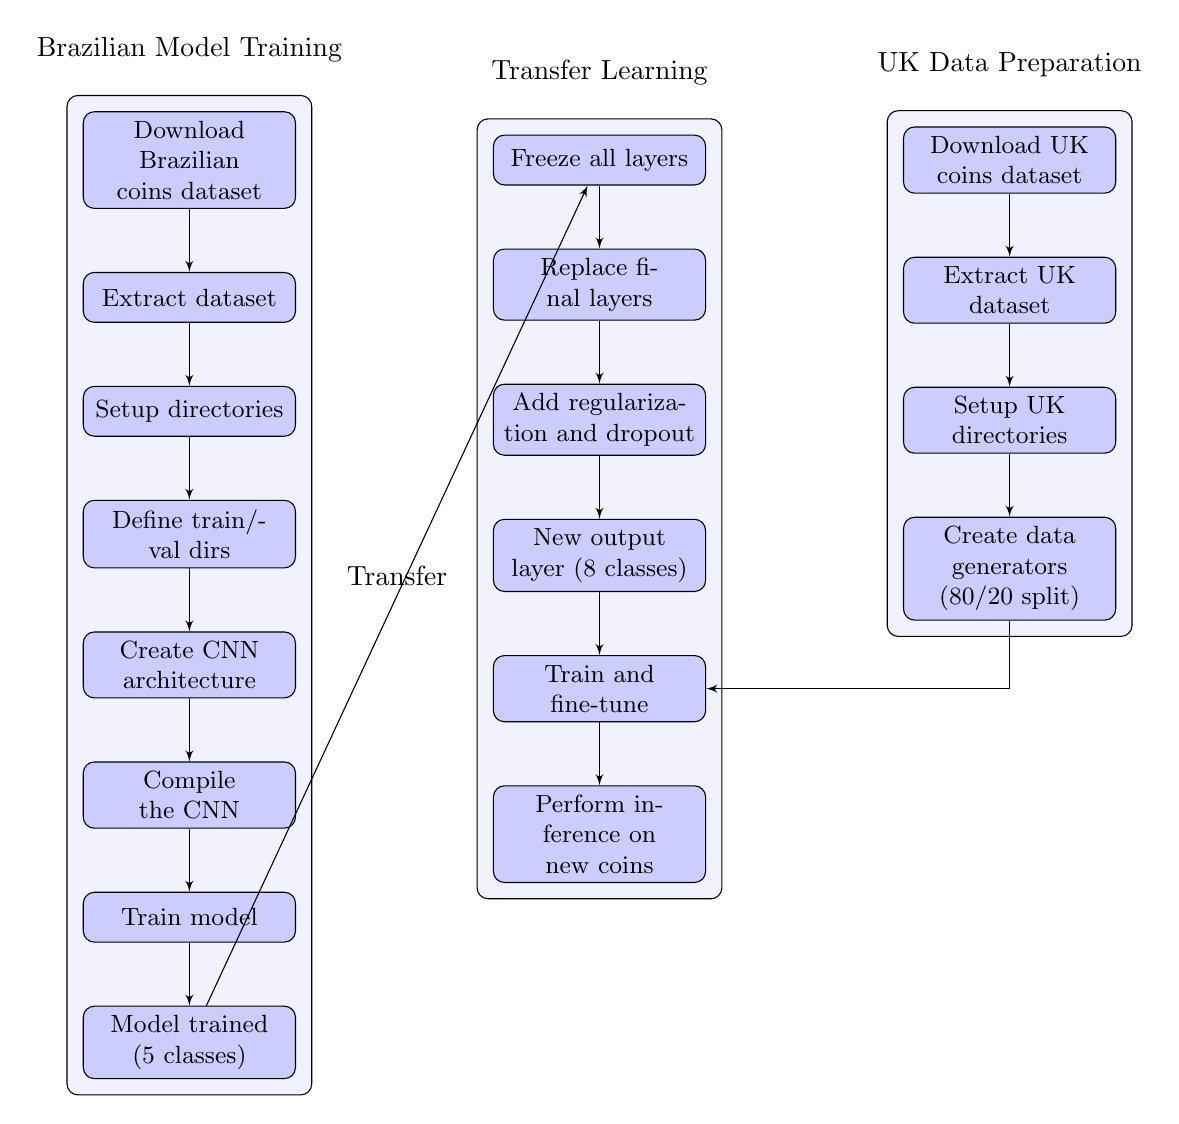
\begin{tikzpicture}[node distance=0.8cm and 1.5cm, auto]
    % Define a smaller block style
    \tikzset{
      block/.style = {rectangle, draw, fill=blue!20, 
                      text width=7em, text centered, rounded corners, minimum height=1.8em, font=\small},
    }
    
    % Brazilian model training - Column 1
    \node [block] (brazildata) {Download Brazilian coins dataset};
    \node [block, below=of brazildata] (extract) {Extract dataset};
    \node [block, below=of extract] (setup) {Setup directories};
    \node [block, below=of setup] (define) {Define train/val dirs};
    \node [block, below=of define] (create) {Create CNN architecture};
    \node [block, below=of create] (compile) {Compile the CNN};
    \node [block, below=of compile] (train) {Train model};
    \node [block, below=of train] (trained) {Model trained (5 classes)};
    
    % Transfer learning - Column 2 (Middle)
    \node [block, right=2.5cm of brazildata] (freeze) {Freeze all layers};
    \node [block, below=of freeze] (replace) {Replace final layers};
    \node [block, below=of replace] (add) {Add regularization and dropout};
    \node [block, below=of add] (output) {New output layer (8 classes)};
    \node [block, below=of output] (finaltrain) {Train and fine-tune};
    \node [block, below=of finaltrain] (inference) {Perform inference on new coins};
    
    % UK data preparation - Column 3 (Right)
    \node [block, right=2.5cm of freeze] (ukdata) {Download UK coins dataset};
    \node [block, below=of ukdata] (ukextract) {Extract UK dataset};
    \node [block, below=of ukextract] (uksetup) {Setup UK directories};
    \node [block, below=of uksetup] (ukgen) {Create data generators (80/20 split)};
    
    % Connect all nodes with arrows
    \path [line] (brazildata) -- (extract);
    \path [line] (extract) -- (setup);
    \path [line] (setup) -- (define);
    \path [line] (define) -- (create);
    \path [line] (create) -- (compile);
    \path [line] (compile) -- (train);
    \path [line] (train) -- (trained);
    
    \path [line] (ukdata) -- (ukextract);
    \path [line] (ukextract) -- (uksetup);
    \path [line] (uksetup) -- (ukgen);
    
    % Connect the columns
    \path [line] (trained) -- node[midway, above] {Transfer} (freeze);
    \path [line] (ukgen) |- (finaltrain);
    
    % Connect middle column
    \path [line] (freeze) -- (replace);
    \path [line] (replace) -- (add);
    \path [line] (add) -- (output);
    \path [line] (output) -- (finaltrain);
    \path [line] (finaltrain) -- (inference);
    
    % Group boxes to show different stages with smaller padding
    \begin{pgfonlayer}{background}
        \node[group={[yshift=0.3cm]above:Brazilian Model Training}, fit={(brazildata) (extract) (setup) (define) (create) (compile) (train) (trained)}, inner sep=0.2cm] {};
        \node[group={[yshift=0.3cm]above:UK Data Preparation}, fit={(ukdata) (ukextract) (uksetup) (ukgen)}, inner sep=0.2cm] {};
        \node[group={[yshift=0.3cm]above:Transfer Learning}, fit={(freeze) (replace) (add) (output) (finaltrain) (inference)}, inner sep=0.2cm] {};
    \end{pgfonlayer}
\end{tikzpicture}
}
% \caption{CNN Transfer Learning Flowchart: Brazilian to UK Coins}
% \label{fig:cnn-flowchart}
% \end{figure}
    }
    \caption{System Design Overview Flowchart}
    \label{fig:decriptiveLabel66} % descriptive to call in text with \ref{fig:decriptiveLabel66}
\end{figure}

\subsection{Functional Requirements}
% Your content here

\subsection{Design Approach}
% Your content here

\subsection{System Architecture}
As shown in Figure~\ref{fig:decriptiveLabel66} the system architecture consists of various components.

\begin{lstlisting}[style=cstyle, caption=System Architecture Code Example, label=lst:SystemArchitecture12]
# Your code here
\end{lstlisting}

\begin{figure}[htbp] %h-ere t-op b-ottom p-page (separte) -good to allow all htbp to give the compiler more options
    \centering
    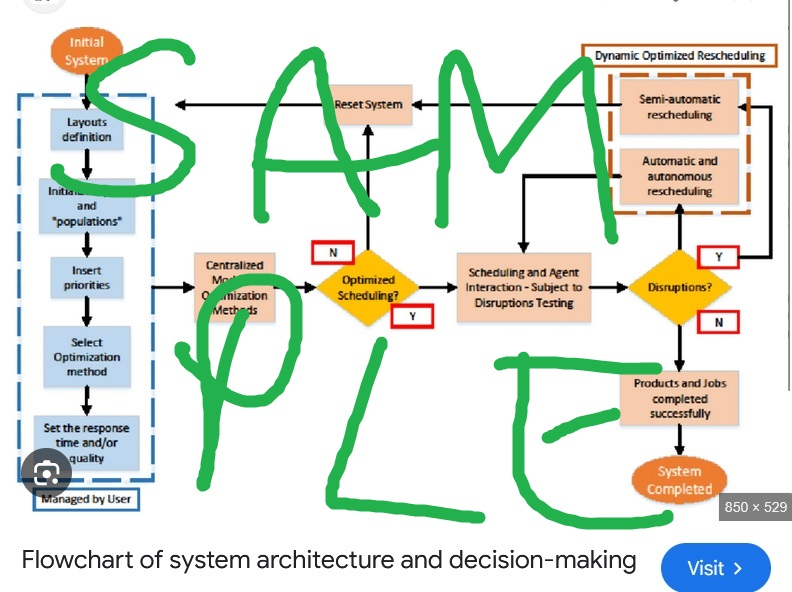
\includegraphics[width=0.6\textwidth]{figures/methodology/system_architecture.jpg}
    \caption{System Architecture Diagram}
    \label{fig:system-architecture7}
\end{figure}
% EnclosureDesignAndFabrication.tex
\section{Enclosure Design And Fabrication}
This section provides an overview of the Enclosure Design And Fabrication.

% Include a flowchart
\begin{figure}[H]
    \centering
    \scalebox{0.8}{ % Scale to 80% of original size
        % try generating flowcharts as svg in Claude 
% and edit with inkscape instead of this.
% but claude did generate this one so might 
% be useful too but you can't easily make
% small repairs in inkscape


% CNN Transfer Learning Flowchart - Compact Multi-Column Layout
% \begin{figure}[htbp]

\centering
\resizebox{\textwidth}{!}{ % Scale to fit width while maintaining aspect ratio
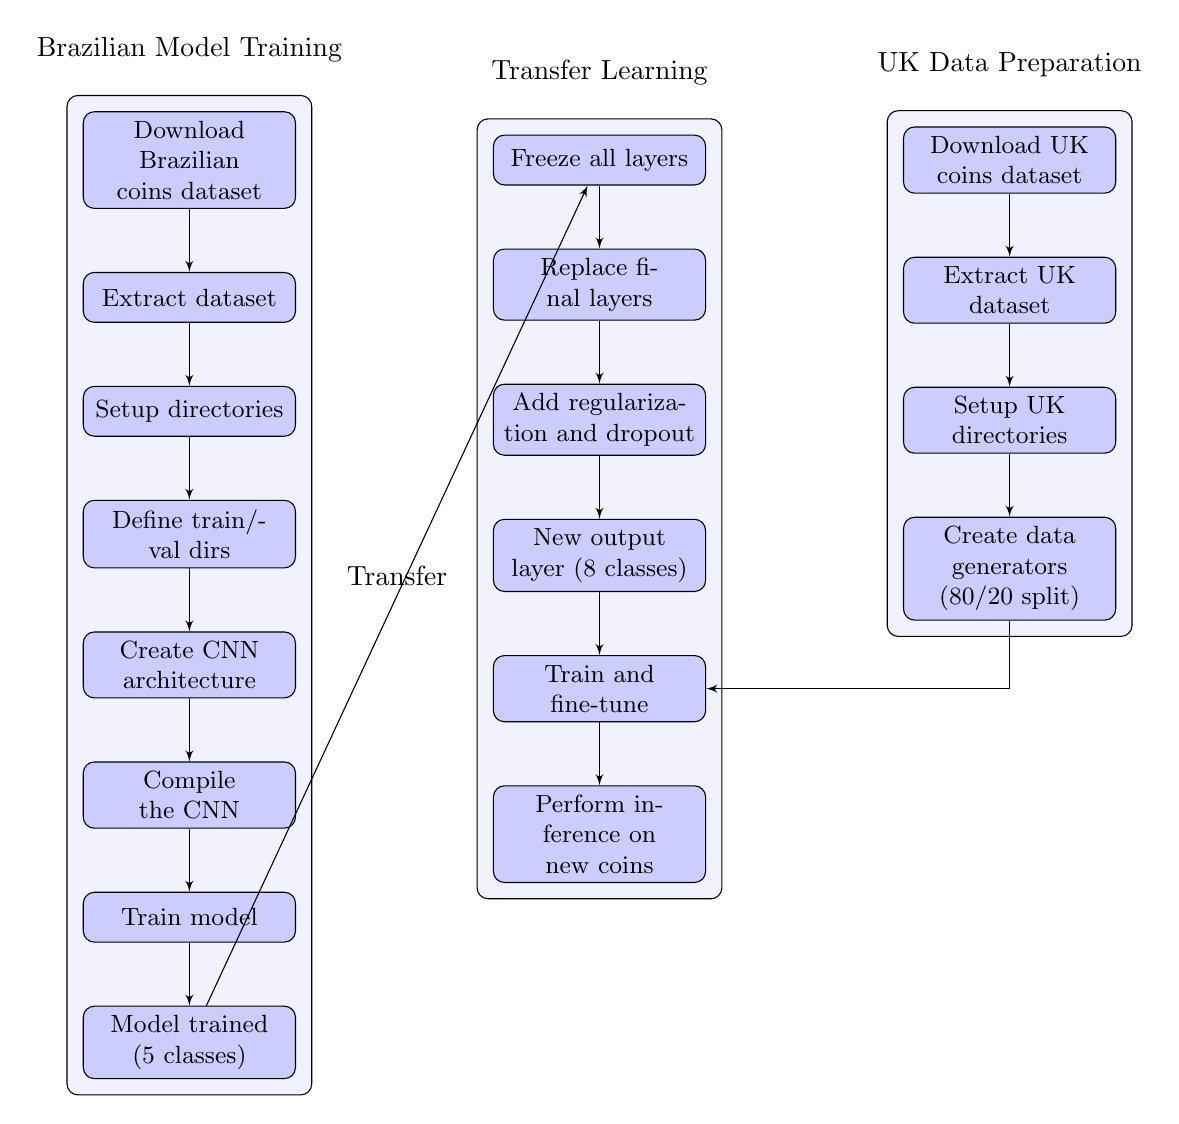
\begin{tikzpicture}[node distance=0.8cm and 1.5cm, auto]
    % Define a smaller block style
    \tikzset{
      block/.style = {rectangle, draw, fill=blue!20, 
                      text width=7em, text centered, rounded corners, minimum height=1.8em, font=\small},
    }
    
    % Brazilian model training - Column 1
    \node [block] (brazildata) {Download Brazilian coins dataset};
    \node [block, below=of brazildata] (extract) {Extract dataset};
    \node [block, below=of extract] (setup) {Setup directories};
    \node [block, below=of setup] (define) {Define train/val dirs};
    \node [block, below=of define] (create) {Create CNN architecture};
    \node [block, below=of create] (compile) {Compile the CNN};
    \node [block, below=of compile] (train) {Train model};
    \node [block, below=of train] (trained) {Model trained (5 classes)};
    
    % Transfer learning - Column 2 (Middle)
    \node [block, right=2.5cm of brazildata] (freeze) {Freeze all layers};
    \node [block, below=of freeze] (replace) {Replace final layers};
    \node [block, below=of replace] (add) {Add regularization and dropout};
    \node [block, below=of add] (output) {New output layer (8 classes)};
    \node [block, below=of output] (finaltrain) {Train and fine-tune};
    \node [block, below=of finaltrain] (inference) {Perform inference on new coins};
    
    % UK data preparation - Column 3 (Right)
    \node [block, right=2.5cm of freeze] (ukdata) {Download UK coins dataset};
    \node [block, below=of ukdata] (ukextract) {Extract UK dataset};
    \node [block, below=of ukextract] (uksetup) {Setup UK directories};
    \node [block, below=of uksetup] (ukgen) {Create data generators (80/20 split)};
    
    % Connect all nodes with arrows
    \path [line] (brazildata) -- (extract);
    \path [line] (extract) -- (setup);
    \path [line] (setup) -- (define);
    \path [line] (define) -- (create);
    \path [line] (create) -- (compile);
    \path [line] (compile) -- (train);
    \path [line] (train) -- (trained);
    
    \path [line] (ukdata) -- (ukextract);
    \path [line] (ukextract) -- (uksetup);
    \path [line] (uksetup) -- (ukgen);
    
    % Connect the columns
    \path [line] (trained) -- node[midway, above] {Transfer} (freeze);
    \path [line] (ukgen) |- (finaltrain);
    
    % Connect middle column
    \path [line] (freeze) -- (replace);
    \path [line] (replace) -- (add);
    \path [line] (add) -- (output);
    \path [line] (output) -- (finaltrain);
    \path [line] (finaltrain) -- (inference);
    
    % Group boxes to show different stages with smaller padding
    \begin{pgfonlayer}{background}
        \node[group={[yshift=0.3cm]above:Brazilian Model Training}, fit={(brazildata) (extract) (setup) (define) (create) (compile) (train) (trained)}, inner sep=0.2cm] {};
        \node[group={[yshift=0.3cm]above:UK Data Preparation}, fit={(ukdata) (ukextract) (uksetup) (ukgen)}, inner sep=0.2cm] {};
        \node[group={[yshift=0.3cm]above:Transfer Learning}, fit={(freeze) (replace) (add) (output) (finaltrain) (inference)}, inner sep=0.2cm] {};
    \end{pgfonlayer}
\end{tikzpicture}
}
% \caption{CNN Transfer Learning Flowchart: Brazilian to UK Coins}
% \label{fig:cnn-flowchart}
% \end{figure}
    }
    \caption{System Design Overview Flowchart}
    \label{fig:decriptiveLabel33} % descriptive to call in text with \ref{fig:decriptiveLabel33}
\end{figure}

\subsection{Functional Requirements}
% Your content here

\subsection{Design Approach}
% Your content here

\subsection{System Architecture}
As shown in Figure~\ref{fig:decriptiveLabel33} the system architecture consists of various components.

\begin{lstlisting}[style=cstyle, caption=System Architecture Code Example, label=lst:SystemArchitecture9]
# Your code here
\end{lstlisting}

\begin{figure}[htbp] %h-ere t-op b-ottom p-page (separte) -good to allow all htbp to give the compiler more options
    \centering
    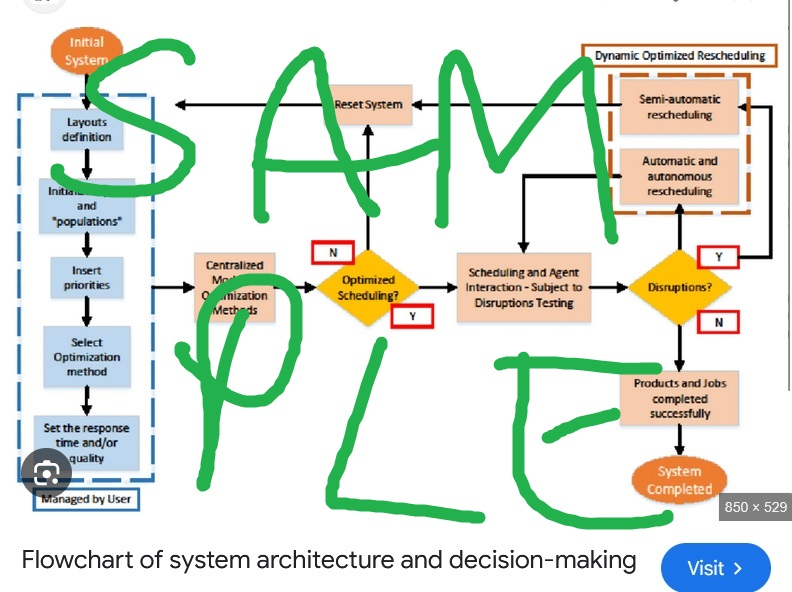
\includegraphics[width=0.6\textwidth]{figures/methodology/system_architecture.jpg}
    \caption{System Architecture Diagram}
    \label{fig:system-architecture4}
\end{figure}
% DataAcquisitionSystem.tex
\section{Data Acquisition System}
This section provides an overview of the Data Acquisition System.

% Include a flowchart in TEX mode
\begin{figure}[H]
    \centering
    \scalebox{0.8}{ % Scale to 80% of original size
        % try generating flowcharts as svg in Claude 
% and edit with inkscape instead of this.
% but claude did generate this one so might 
% be useful too but you can't easily make
% small repairs in inkscape


% CNN Transfer Learning Flowchart - Compact Multi-Column Layout
% \begin{figure}[htbp]

\centering
\resizebox{\textwidth}{!}{ % Scale to fit width while maintaining aspect ratio
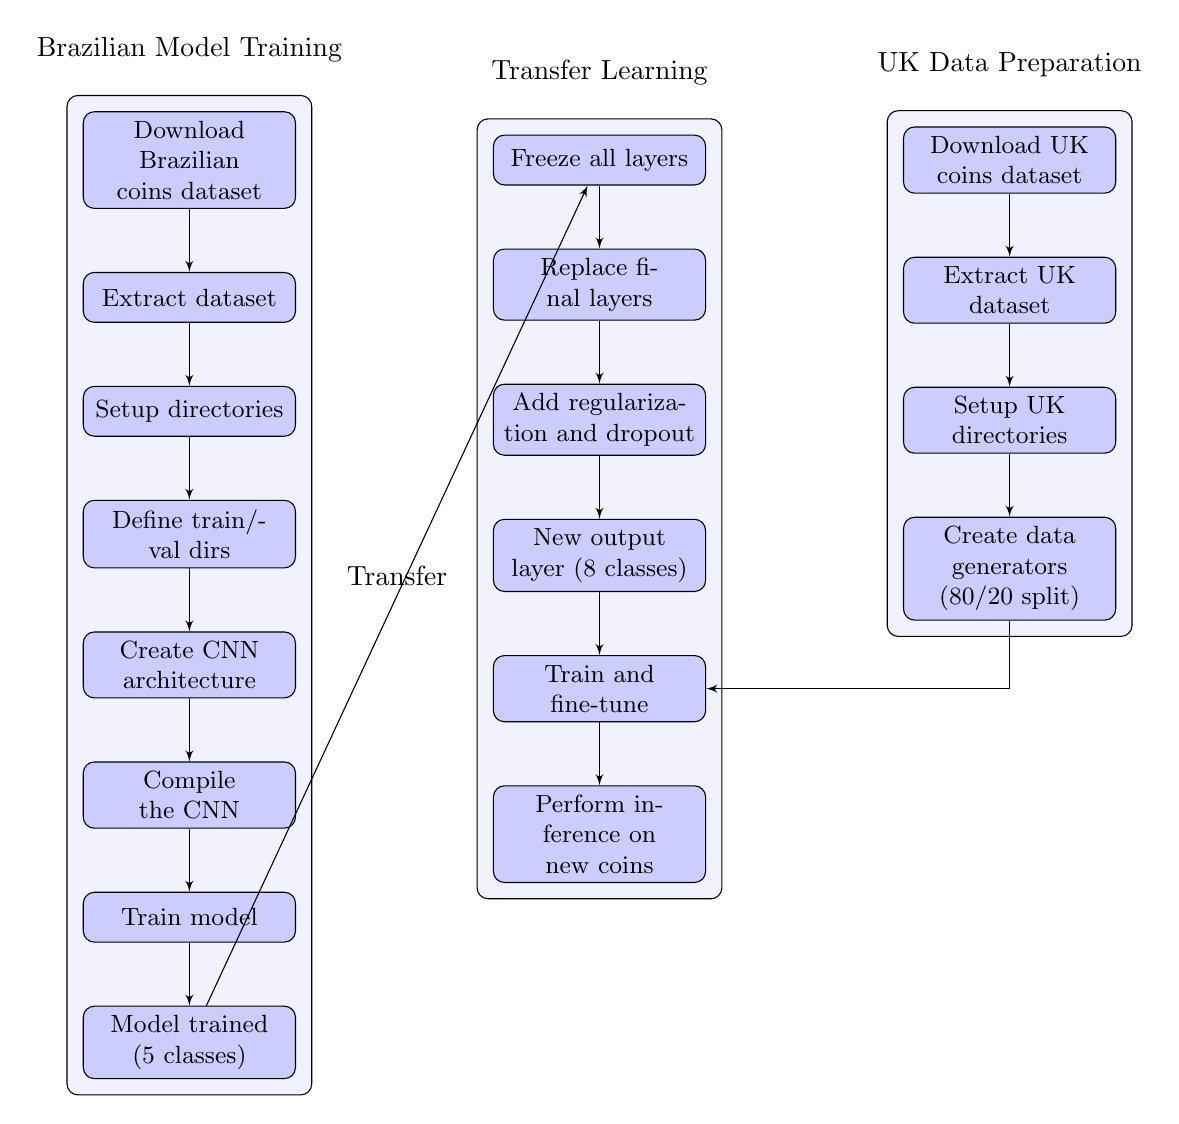
\begin{tikzpicture}[node distance=0.8cm and 1.5cm, auto]
    % Define a smaller block style
    \tikzset{
      block/.style = {rectangle, draw, fill=blue!20, 
                      text width=7em, text centered, rounded corners, minimum height=1.8em, font=\small},
    }
    
    % Brazilian model training - Column 1
    \node [block] (brazildata) {Download Brazilian coins dataset};
    \node [block, below=of brazildata] (extract) {Extract dataset};
    \node [block, below=of extract] (setup) {Setup directories};
    \node [block, below=of setup] (define) {Define train/val dirs};
    \node [block, below=of define] (create) {Create CNN architecture};
    \node [block, below=of create] (compile) {Compile the CNN};
    \node [block, below=of compile] (train) {Train model};
    \node [block, below=of train] (trained) {Model trained (5 classes)};
    
    % Transfer learning - Column 2 (Middle)
    \node [block, right=2.5cm of brazildata] (freeze) {Freeze all layers};
    \node [block, below=of freeze] (replace) {Replace final layers};
    \node [block, below=of replace] (add) {Add regularization and dropout};
    \node [block, below=of add] (output) {New output layer (8 classes)};
    \node [block, below=of output] (finaltrain) {Train and fine-tune};
    \node [block, below=of finaltrain] (inference) {Perform inference on new coins};
    
    % UK data preparation - Column 3 (Right)
    \node [block, right=2.5cm of freeze] (ukdata) {Download UK coins dataset};
    \node [block, below=of ukdata] (ukextract) {Extract UK dataset};
    \node [block, below=of ukextract] (uksetup) {Setup UK directories};
    \node [block, below=of uksetup] (ukgen) {Create data generators (80/20 split)};
    
    % Connect all nodes with arrows
    \path [line] (brazildata) -- (extract);
    \path [line] (extract) -- (setup);
    \path [line] (setup) -- (define);
    \path [line] (define) -- (create);
    \path [line] (create) -- (compile);
    \path [line] (compile) -- (train);
    \path [line] (train) -- (trained);
    
    \path [line] (ukdata) -- (ukextract);
    \path [line] (ukextract) -- (uksetup);
    \path [line] (uksetup) -- (ukgen);
    
    % Connect the columns
    \path [line] (trained) -- node[midway, above] {Transfer} (freeze);
    \path [line] (ukgen) |- (finaltrain);
    
    % Connect middle column
    \path [line] (freeze) -- (replace);
    \path [line] (replace) -- (add);
    \path [line] (add) -- (output);
    \path [line] (output) -- (finaltrain);
    \path [line] (finaltrain) -- (inference);
    
    % Group boxes to show different stages with smaller padding
    \begin{pgfonlayer}{background}
        \node[group={[yshift=0.3cm]above:Brazilian Model Training}, fit={(brazildata) (extract) (setup) (define) (create) (compile) (train) (trained)}, inner sep=0.2cm] {};
        \node[group={[yshift=0.3cm]above:UK Data Preparation}, fit={(ukdata) (ukextract) (uksetup) (ukgen)}, inner sep=0.2cm] {};
        \node[group={[yshift=0.3cm]above:Transfer Learning}, fit={(freeze) (replace) (add) (output) (finaltrain) (inference)}, inner sep=0.2cm] {};
    \end{pgfonlayer}
\end{tikzpicture}
}
% \caption{CNN Transfer Learning Flowchart: Brazilian to UK Coins}
% \label{fig:cnn-flowchart}
% \end{figure} % \input is for tex files \includegraphics is for images
    }
    \caption{System Design Overview Flowchart}
    \label{fig:decriptiveLabel22} % descriptive to call in text with \ref{fig:decriptiveLabel22}
\end{figure}


% other subsections
\subsection{Functional Requirements}
% Your content here

\subsection{Design Approach}
% Your content here

\subsection{System Architecture}
As shown in Figure~\ref{fig:decriptiveLabel22} the system architecture consists of various components.

\begin{lstlisting}[style=cstyle, caption=System Architecture Code Example, label=lst:SystemArchitecture8]
# Your code here
\end{lstlisting}

\begin{figure}[htbp] %h-ere t-op b-ottom p-page (separte) -good to allow all htbp to give the compiler more options
    \centering
    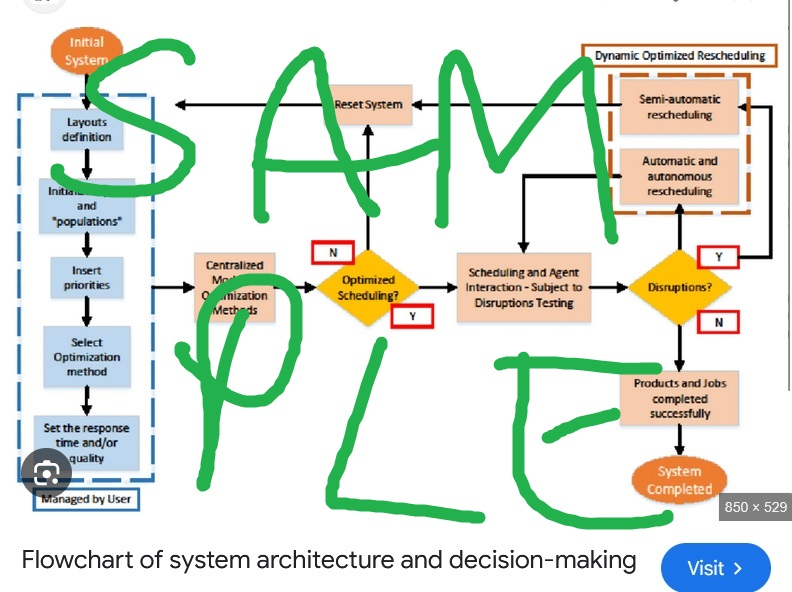
\includegraphics[width=0.6\textwidth]{figures/methodology/system_architecture.jpg}
    \caption{System Architecture Diagram}
    \label{fig:system-architecture3}
\end{figure}
% TestingApparatus.tex
\section{Testing Apparatus}
This section provides an overview of the Testing Apparatus.

% Include a flowchart
\begin{figure}[H]
    \centering
    \scalebox{0.8}{ % Scale to 80% of original size
        % try generating flowcharts as svg in Claude 
% and edit with inkscape instead of this.
% but claude did generate this one so might 
% be useful too but you can't easily make
% small repairs in inkscape


% CNN Transfer Learning Flowchart - Compact Multi-Column Layout
% \begin{figure}[htbp]

\centering
\resizebox{\textwidth}{!}{ % Scale to fit width while maintaining aspect ratio
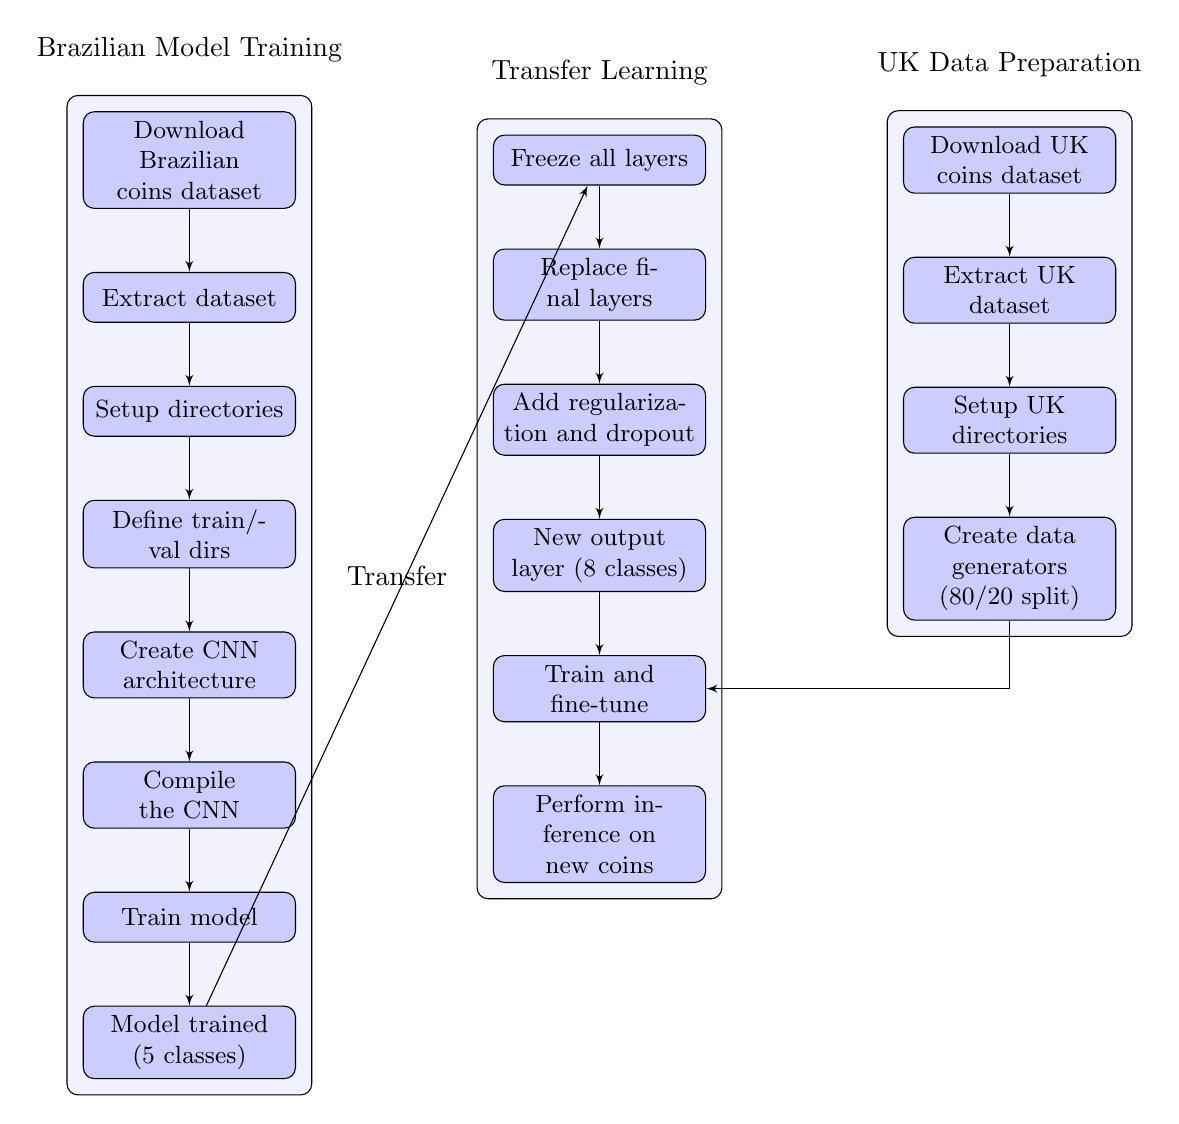
\begin{tikzpicture}[node distance=0.8cm and 1.5cm, auto]
    % Define a smaller block style
    \tikzset{
      block/.style = {rectangle, draw, fill=blue!20, 
                      text width=7em, text centered, rounded corners, minimum height=1.8em, font=\small},
    }
    
    % Brazilian model training - Column 1
    \node [block] (brazildata) {Download Brazilian coins dataset};
    \node [block, below=of brazildata] (extract) {Extract dataset};
    \node [block, below=of extract] (setup) {Setup directories};
    \node [block, below=of setup] (define) {Define train/val dirs};
    \node [block, below=of define] (create) {Create CNN architecture};
    \node [block, below=of create] (compile) {Compile the CNN};
    \node [block, below=of compile] (train) {Train model};
    \node [block, below=of train] (trained) {Model trained (5 classes)};
    
    % Transfer learning - Column 2 (Middle)
    \node [block, right=2.5cm of brazildata] (freeze) {Freeze all layers};
    \node [block, below=of freeze] (replace) {Replace final layers};
    \node [block, below=of replace] (add) {Add regularization and dropout};
    \node [block, below=of add] (output) {New output layer (8 classes)};
    \node [block, below=of output] (finaltrain) {Train and fine-tune};
    \node [block, below=of finaltrain] (inference) {Perform inference on new coins};
    
    % UK data preparation - Column 3 (Right)
    \node [block, right=2.5cm of freeze] (ukdata) {Download UK coins dataset};
    \node [block, below=of ukdata] (ukextract) {Extract UK dataset};
    \node [block, below=of ukextract] (uksetup) {Setup UK directories};
    \node [block, below=of uksetup] (ukgen) {Create data generators (80/20 split)};
    
    % Connect all nodes with arrows
    \path [line] (brazildata) -- (extract);
    \path [line] (extract) -- (setup);
    \path [line] (setup) -- (define);
    \path [line] (define) -- (create);
    \path [line] (create) -- (compile);
    \path [line] (compile) -- (train);
    \path [line] (train) -- (trained);
    
    \path [line] (ukdata) -- (ukextract);
    \path [line] (ukextract) -- (uksetup);
    \path [line] (uksetup) -- (ukgen);
    
    % Connect the columns
    \path [line] (trained) -- node[midway, above] {Transfer} (freeze);
    \path [line] (ukgen) |- (finaltrain);
    
    % Connect middle column
    \path [line] (freeze) -- (replace);
    \path [line] (replace) -- (add);
    \path [line] (add) -- (output);
    \path [line] (output) -- (finaltrain);
    \path [line] (finaltrain) -- (inference);
    
    % Group boxes to show different stages with smaller padding
    \begin{pgfonlayer}{background}
        \node[group={[yshift=0.3cm]above:Brazilian Model Training}, fit={(brazildata) (extract) (setup) (define) (create) (compile) (train) (trained)}, inner sep=0.2cm] {};
        \node[group={[yshift=0.3cm]above:UK Data Preparation}, fit={(ukdata) (ukextract) (uksetup) (ukgen)}, inner sep=0.2cm] {};
        \node[group={[yshift=0.3cm]above:Transfer Learning}, fit={(freeze) (replace) (add) (output) (finaltrain) (inference)}, inner sep=0.2cm] {};
    \end{pgfonlayer}
\end{tikzpicture}
}
% \caption{CNN Transfer Learning Flowchart: Brazilian to UK Coins}
% \label{fig:cnn-flowchart}
% \end{figure}
    }
    \caption{System Design Overview Flowchart}
    \label{fig:decriptiveLabel11} % descriptive to call in text with \ref{fig:decriptiveLabel}
\end{figure}

\subsection{Functional Requirements}
% Your content here

\subsection{Design Approach}
% Your content here

\subsection{System Architecture}
As shown in Figure~\ref{fig:decriptiveLabel11} the system architecture consists of various components.

\begin{lstlisting}[style=cstyle, caption=System Architecture Code Example, label=lst:SystemArchitecture7]
# Your code here
\end{lstlisting}

\begin{figure}[htbp] %h-ere t-op b-ottom p-page (separte) -good to allow all htbp to give the compiler more options
    \centering
    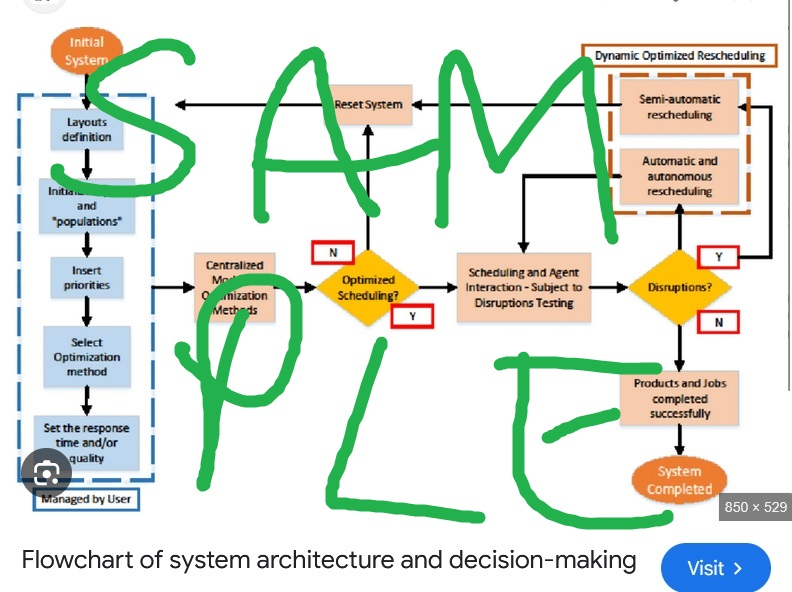
\includegraphics[width=0.6\textwidth]{figures/methodology/system_architecture.jpg}
    \caption{System Architecture Diagram}
    \label{fig:system-architecture2}
\end{figure}
% PrototypeDevelopmentLifecycle.tex
\section{Prototype Develop ment Lifecycle}
This section provides an overview of the Prototype Develop ment Lifecycle.

% Include a flowchart
\begin{figure}[H]
    \centering
    \scalebox{0.8}{ % Scale to 80% of original size
        % try generating flowcharts as svg in Claude 
% and edit with inkscape instead of this.
% but claude did generate this one so might 
% be useful too but you can't easily make
% small repairs in inkscape


% CNN Transfer Learning Flowchart - Compact Multi-Column Layout
% \begin{figure}[htbp]

\centering
\resizebox{\textwidth}{!}{ % Scale to fit width while maintaining aspect ratio
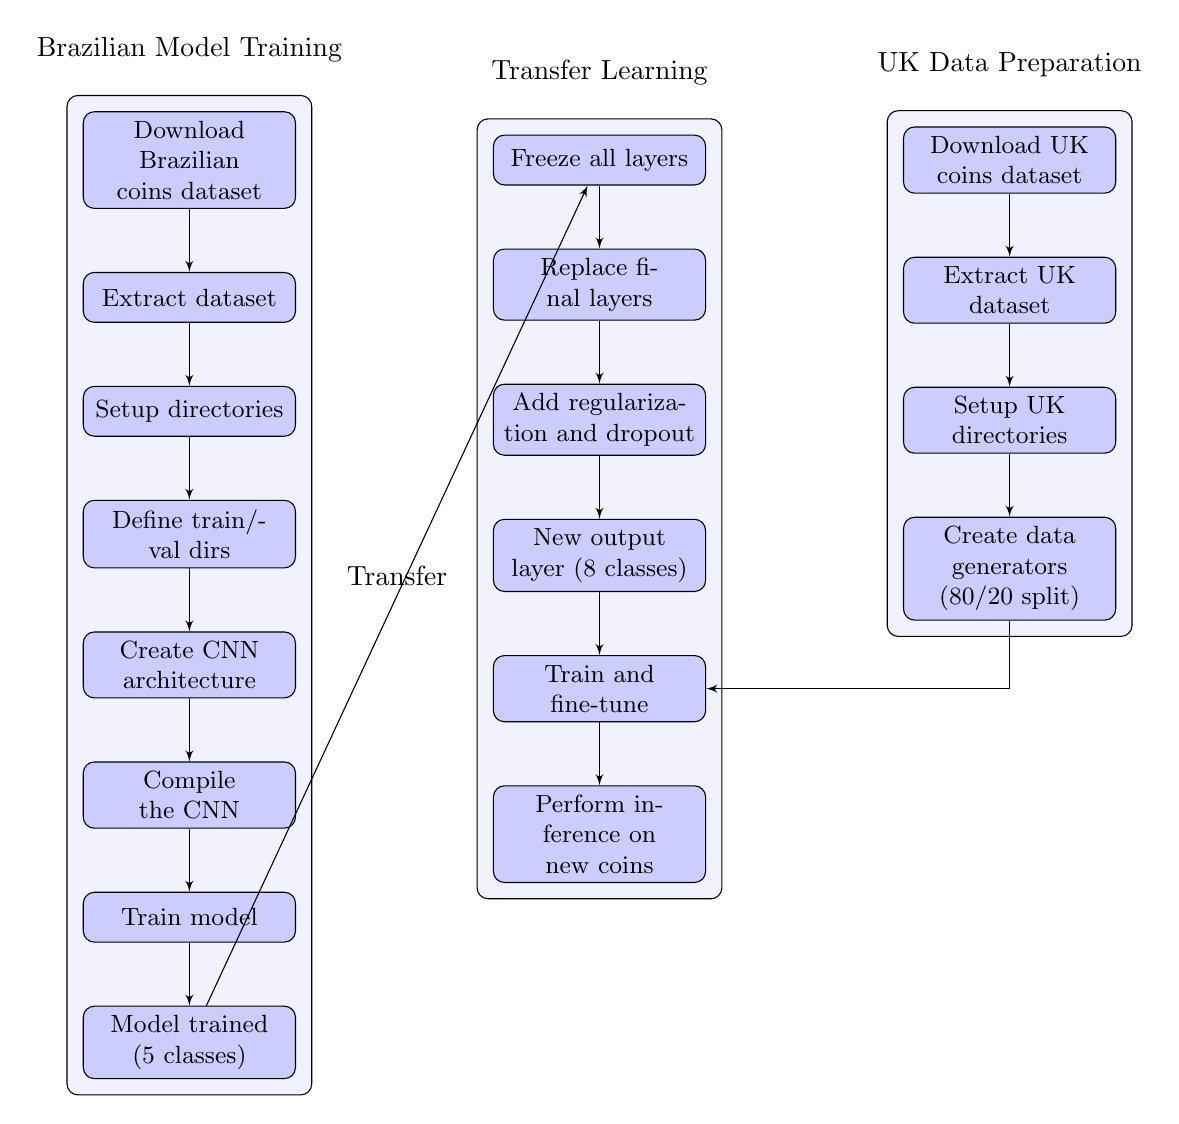
\begin{tikzpicture}[node distance=0.8cm and 1.5cm, auto]
    % Define a smaller block style
    \tikzset{
      block/.style = {rectangle, draw, fill=blue!20, 
                      text width=7em, text centered, rounded corners, minimum height=1.8em, font=\small},
    }
    
    % Brazilian model training - Column 1
    \node [block] (brazildata) {Download Brazilian coins dataset};
    \node [block, below=of brazildata] (extract) {Extract dataset};
    \node [block, below=of extract] (setup) {Setup directories};
    \node [block, below=of setup] (define) {Define train/val dirs};
    \node [block, below=of define] (create) {Create CNN architecture};
    \node [block, below=of create] (compile) {Compile the CNN};
    \node [block, below=of compile] (train) {Train model};
    \node [block, below=of train] (trained) {Model trained (5 classes)};
    
    % Transfer learning - Column 2 (Middle)
    \node [block, right=2.5cm of brazildata] (freeze) {Freeze all layers};
    \node [block, below=of freeze] (replace) {Replace final layers};
    \node [block, below=of replace] (add) {Add regularization and dropout};
    \node [block, below=of add] (output) {New output layer (8 classes)};
    \node [block, below=of output] (finaltrain) {Train and fine-tune};
    \node [block, below=of finaltrain] (inference) {Perform inference on new coins};
    
    % UK data preparation - Column 3 (Right)
    \node [block, right=2.5cm of freeze] (ukdata) {Download UK coins dataset};
    \node [block, below=of ukdata] (ukextract) {Extract UK dataset};
    \node [block, below=of ukextract] (uksetup) {Setup UK directories};
    \node [block, below=of uksetup] (ukgen) {Create data generators (80/20 split)};
    
    % Connect all nodes with arrows
    \path [line] (brazildata) -- (extract);
    \path [line] (extract) -- (setup);
    \path [line] (setup) -- (define);
    \path [line] (define) -- (create);
    \path [line] (create) -- (compile);
    \path [line] (compile) -- (train);
    \path [line] (train) -- (trained);
    
    \path [line] (ukdata) -- (ukextract);
    \path [line] (ukextract) -- (uksetup);
    \path [line] (uksetup) -- (ukgen);
    
    % Connect the columns
    \path [line] (trained) -- node[midway, above] {Transfer} (freeze);
    \path [line] (ukgen) |- (finaltrain);
    
    % Connect middle column
    \path [line] (freeze) -- (replace);
    \path [line] (replace) -- (add);
    \path [line] (add) -- (output);
    \path [line] (output) -- (finaltrain);
    \path [line] (finaltrain) -- (inference);
    
    % Group boxes to show different stages with smaller padding
    \begin{pgfonlayer}{background}
        \node[group={[yshift=0.3cm]above:Brazilian Model Training}, fit={(brazildata) (extract) (setup) (define) (create) (compile) (train) (trained)}, inner sep=0.2cm] {};
        \node[group={[yshift=0.3cm]above:UK Data Preparation}, fit={(ukdata) (ukextract) (uksetup) (ukgen)}, inner sep=0.2cm] {};
        \node[group={[yshift=0.3cm]above:Transfer Learning}, fit={(freeze) (replace) (add) (output) (finaltrain) (inference)}, inner sep=0.2cm] {};
    \end{pgfonlayer}
\end{tikzpicture}
}
% \caption{CNN Transfer Learning Flowchart: Brazilian to UK Coins}
% \label{fig:cnn-flowchart}
% \end{figure}
    }
    \caption{System Design Overview Flowchart}
    \label{fig:decriptiveLabel44} % descriptive to call in text with \ref{fig:decriptiveLabel44}
\end{figure}

\subsection{Functional Requirements}
% Your content here

\subsection{Design Approach}
% Your content here

\subsection{System Architecture}
As shown in Figure~\ref{fig:decriptiveLabel44} the system architecture consists of various components.

\begin{lstlisting}[style=cstyle, caption=System Architecture Code Example, label=lst:SystemArchitecture10]
# Your code here
\end{lstlisting}

\begin{figure}[htbp] %h-ere t-op b-ottom p-page (separte) -good to allow all htbp to give the compiler more options
    \centering
    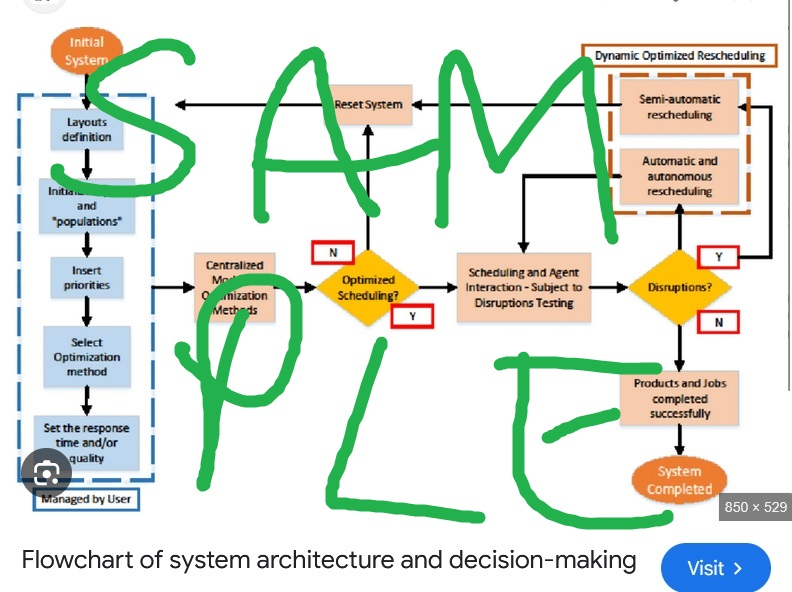
\includegraphics[width=0.6\textwidth]{figures/methodology/system_architecture.jpg}
    \caption{System Architecture Diagram}
    \label{fig:system-architecture5}
\end{figure}


% Results.tex
\chapter{Results}

% Include each section from separate files
% SensorCharacterization.tex
\section{Sensor Characterization}
%
% THIS NEEDS CHANGING
%
%
TO FINISHTO FINISHTO FINISHTO FINISHTO FINISHTO FINISHTO FINISH focus on the fundamental properties and performance of your photodiodes themselves, distinct from the other subsections. Here are some key elements that would belong specifically under SensorCharacterization:

Basic Photodiode Electrical Characteristics:

Dark current measurements
Junction capacitance
I-V characteristics in different lighting conditions
Spectral response profiles (sensitivity vs. wavelength)


Individual Sensor Benchmarking:

Performance comparison between the 4 photodiodes (matching/differences)
Responsivity measurements (A/W)
Quantum efficiency calculations
Detection threshold levels

SNR!

Response Linearity:

Measurements showing linear range of the photodiodes
Saturation point characterization
Recovery time from saturation


Temperature Dependency:

Performance drift with temperature
Baseline shift measurements
Temperature compensation data


Aging/Stability Tests:

Long-term drift measurements
Repeatability of measurements over time



This section should focus on the inherent properties of the photodiodes themselves - essentially providing the baseline characterization data that underpins all the other analysis. The other sections then build on this foundation by examining how these sensors perform when integrated into the complete system with amplification, angular positioning, enclosure effects, etc.




% Example figure jpg
%
% \begin{figure}[htb]
%     \centering
%     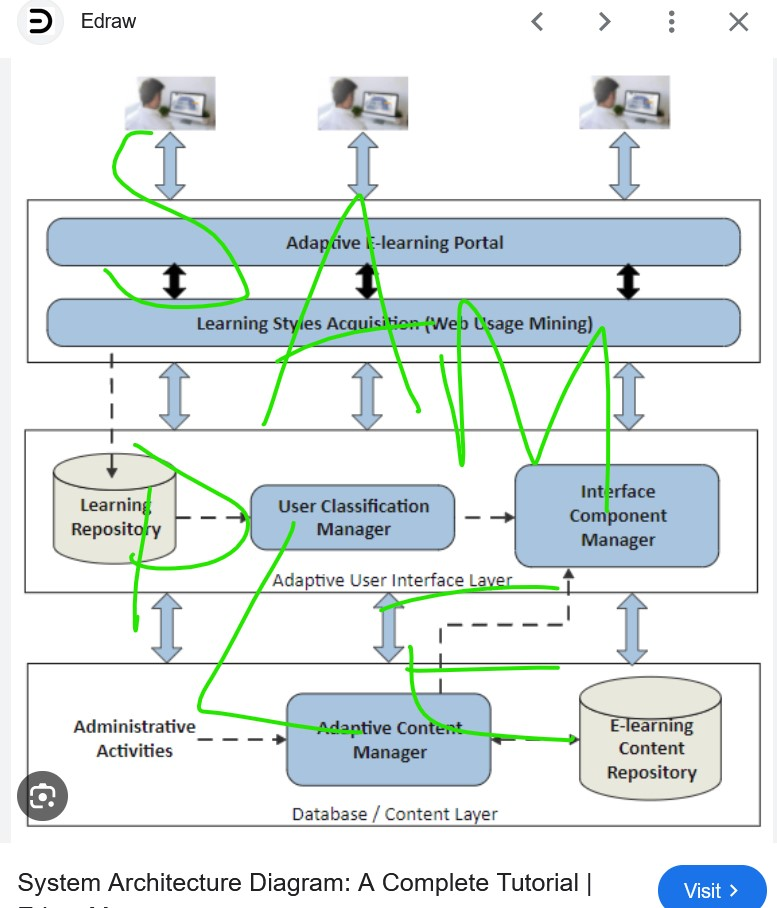
\includegraphics[width=1\textwidth]{figures/results/system_architecture.jpg}
%     \caption{Overall System Performance Analysis}
%     \label{fig:systemPerformance}
% \end{figure}

% Example listing (such as text output from console)
% \begin{figure}[H]
%     \begin{lstlisting}[style=cstyle]
%     // Environmental test results
%     // Temperature, ambient light, and vibration effects
%     \end{lstlisting}
%     \caption{Environmental Testing Results}
%     \label{lst:EnvironmentalTests1}
%     \end{figure}



% LATEX flowchar
% Include a flowchart
% \begin{figure}[H]
%     \centering
%     \scalebox{0.8}{ % Scale to 80% of original size
%         % try generating flowcharts as svg in Claude 
% and edit with inkscape instead of this.
% but claude did generate this one so might 
% be useful too but you can't easily make
% small repairs in inkscape


% CNN Transfer Learning Flowchart - Compact Multi-Column Layout
% \begin{figure}[htbp]

\centering
\resizebox{\textwidth}{!}{ % Scale to fit width while maintaining aspect ratio
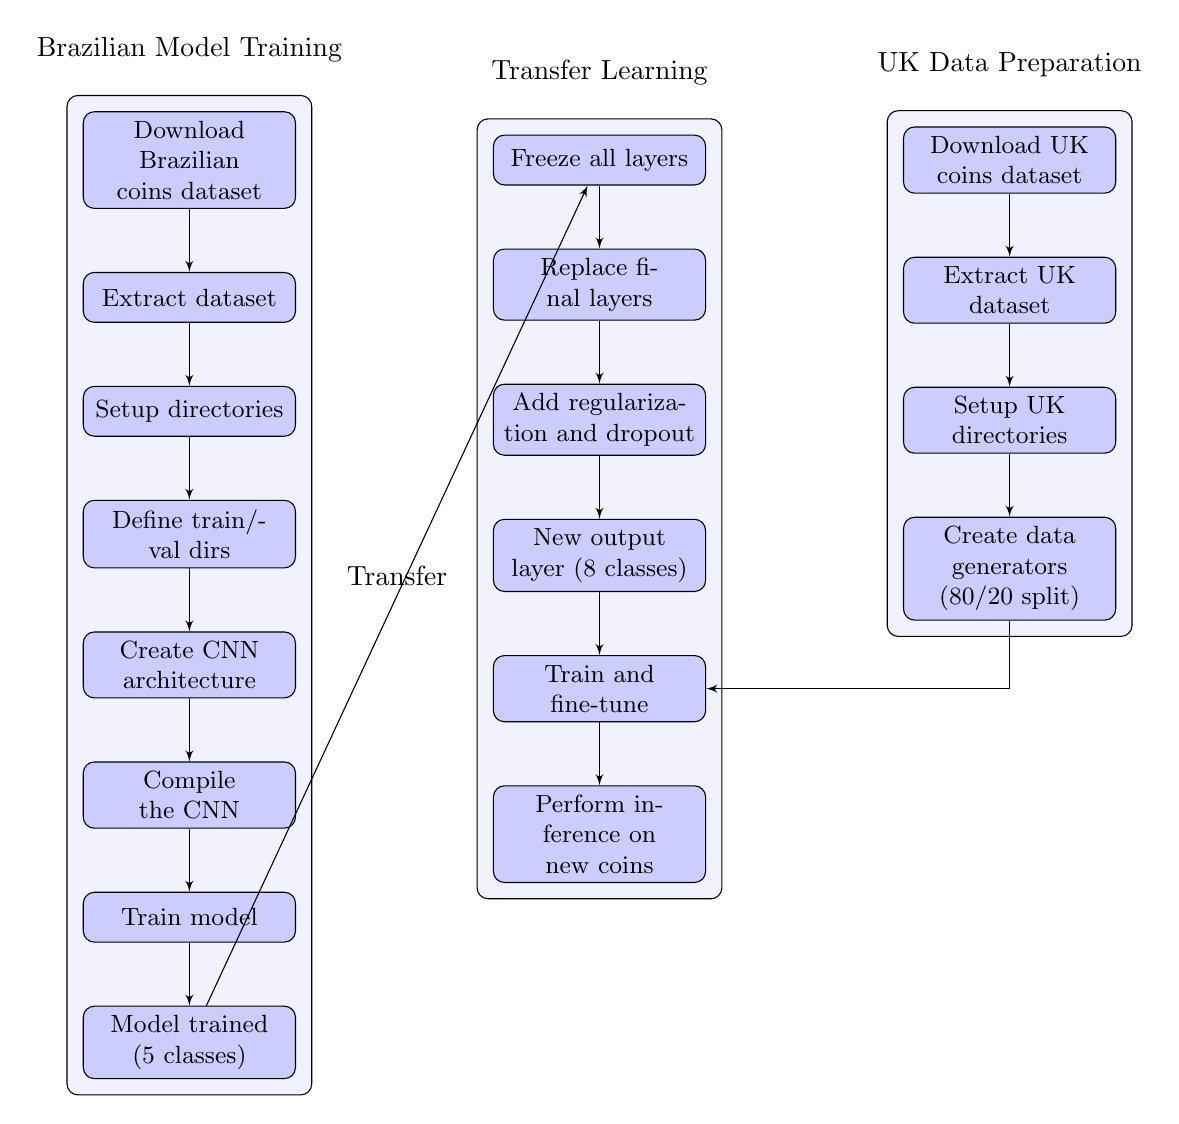
\begin{tikzpicture}[node distance=0.8cm and 1.5cm, auto]
    % Define a smaller block style
    \tikzset{
      block/.style = {rectangle, draw, fill=blue!20, 
                      text width=7em, text centered, rounded corners, minimum height=1.8em, font=\small},
    }
    
    % Brazilian model training - Column 1
    \node [block] (brazildata) {Download Brazilian coins dataset};
    \node [block, below=of brazildata] (extract) {Extract dataset};
    \node [block, below=of extract] (setup) {Setup directories};
    \node [block, below=of setup] (define) {Define train/val dirs};
    \node [block, below=of define] (create) {Create CNN architecture};
    \node [block, below=of create] (compile) {Compile the CNN};
    \node [block, below=of compile] (train) {Train model};
    \node [block, below=of train] (trained) {Model trained (5 classes)};
    
    % Transfer learning - Column 2 (Middle)
    \node [block, right=2.5cm of brazildata] (freeze) {Freeze all layers};
    \node [block, below=of freeze] (replace) {Replace final layers};
    \node [block, below=of replace] (add) {Add regularization and dropout};
    \node [block, below=of add] (output) {New output layer (8 classes)};
    \node [block, below=of output] (finaltrain) {Train and fine-tune};
    \node [block, below=of finaltrain] (inference) {Perform inference on new coins};
    
    % UK data preparation - Column 3 (Right)
    \node [block, right=2.5cm of freeze] (ukdata) {Download UK coins dataset};
    \node [block, below=of ukdata] (ukextract) {Extract UK dataset};
    \node [block, below=of ukextract] (uksetup) {Setup UK directories};
    \node [block, below=of uksetup] (ukgen) {Create data generators (80/20 split)};
    
    % Connect all nodes with arrows
    \path [line] (brazildata) -- (extract);
    \path [line] (extract) -- (setup);
    \path [line] (setup) -- (define);
    \path [line] (define) -- (create);
    \path [line] (create) -- (compile);
    \path [line] (compile) -- (train);
    \path [line] (train) -- (trained);
    
    \path [line] (ukdata) -- (ukextract);
    \path [line] (ukextract) -- (uksetup);
    \path [line] (uksetup) -- (ukgen);
    
    % Connect the columns
    \path [line] (trained) -- node[midway, above] {Transfer} (freeze);
    \path [line] (ukgen) |- (finaltrain);
    
    % Connect middle column
    \path [line] (freeze) -- (replace);
    \path [line] (replace) -- (add);
    \path [line] (add) -- (output);
    \path [line] (output) -- (finaltrain);
    \path [line] (finaltrain) -- (inference);
    
    % Group boxes to show different stages with smaller padding
    \begin{pgfonlayer}{background}
        \node[group={[yshift=0.3cm]above:Brazilian Model Training}, fit={(brazildata) (extract) (setup) (define) (create) (compile) (train) (trained)}, inner sep=0.2cm] {};
        \node[group={[yshift=0.3cm]above:UK Data Preparation}, fit={(ukdata) (ukextract) (uksetup) (ukgen)}, inner sep=0.2cm] {};
        \node[group={[yshift=0.3cm]above:Transfer Learning}, fit={(freeze) (replace) (add) (output) (finaltrain) (inference)}, inner sep=0.2cm] {};
    \end{pgfonlayer}
\end{tikzpicture}
}
% \caption{CNN Transfer Learning Flowchart: Brazilian to UK Coins}
% \label{fig:cnn-flowchart}
% \end{figure}
%     }
%     \caption{System Design Overview Flowchart}
%     \label{fig:decriptiveLabel3} % descriptive to call in text with \ref{fig:decriptiveLabel}
% \end{figure}

% AmplificationPerformance.tex
\section{Amplification Performance}
As seen previously during iteration, the amplification circuit was able to correctly transduce and amplify the current from the photodiodes. The results in complete darkness measurement can be seen in Figure \ref{fig:ampPerf}, the output voltage across all photodiodes is measured at well below 


\begin{figure}[htb]
    \centering
    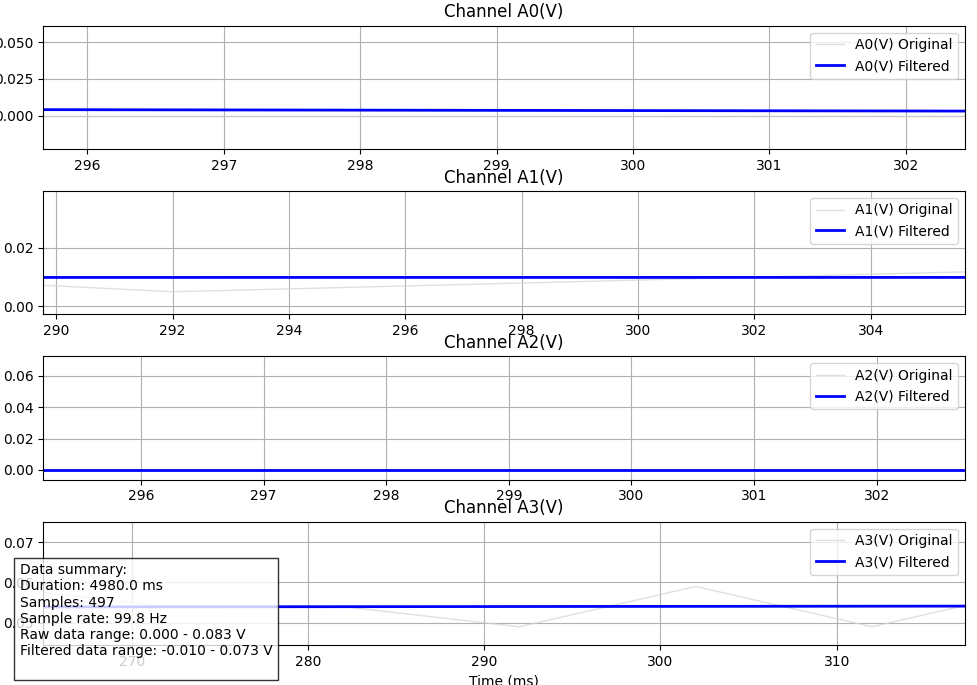
\includegraphics[width=1\textwidth]{chapters/results/images/result_amplification_perf.png}
    \caption{Measurement of Voltage in Complete Darkness}
    \label{fig:ampPerf}
\end{figure}

A recording is displayed in Figure \ref{fig:recZoom} showing the recording of a sampling with the light moving at 0.2Hz with the arch at 90\textdegree and the LED strip going across from near 0\textdegree to near 180\textdegree. This result was considered good, as when compared to simulation, it was very similar, as can be seen in Figure
% zoomed
\begin{figure}[htb]
    \centering
    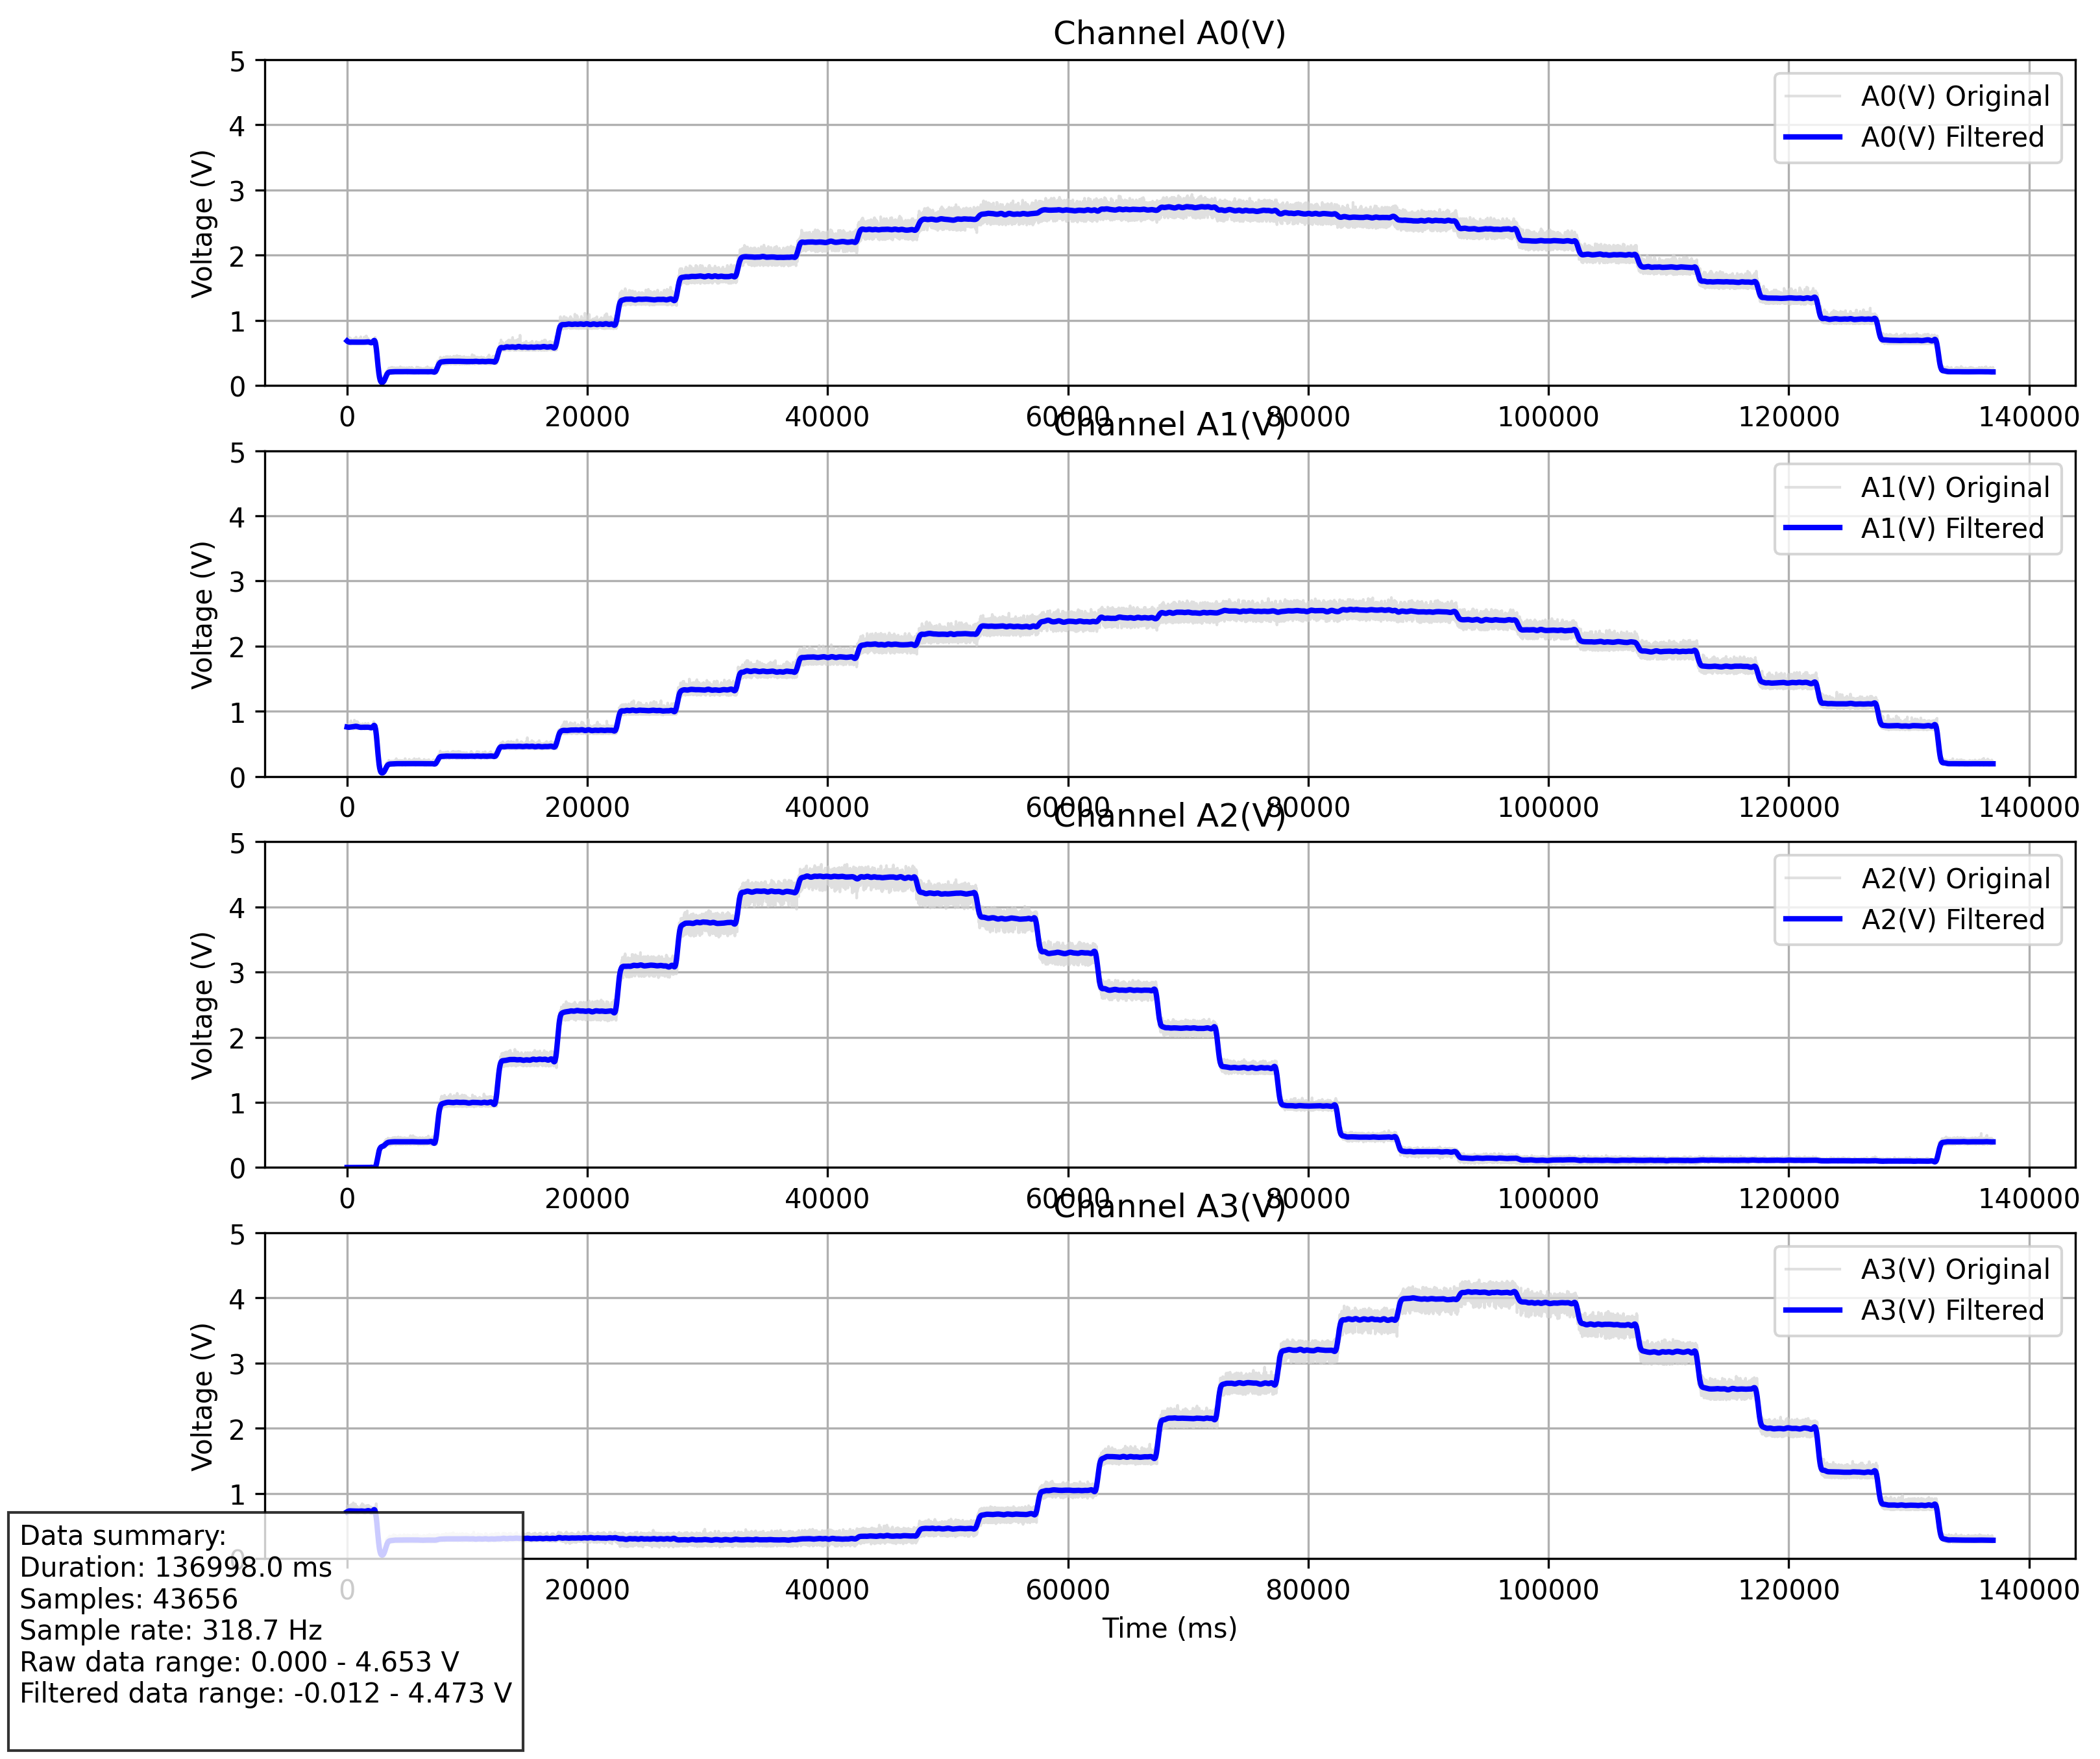
\includegraphics[width=0.6\textwidth]{chapters/results/images/120s_zoomed.png}
    \caption{Measurement of Voltage across 140 seconds}
    \label{fig:recZoom}
\end{figure}

% Example figure jpg
%
% \begin{figure}[htb]
%     \centering
%     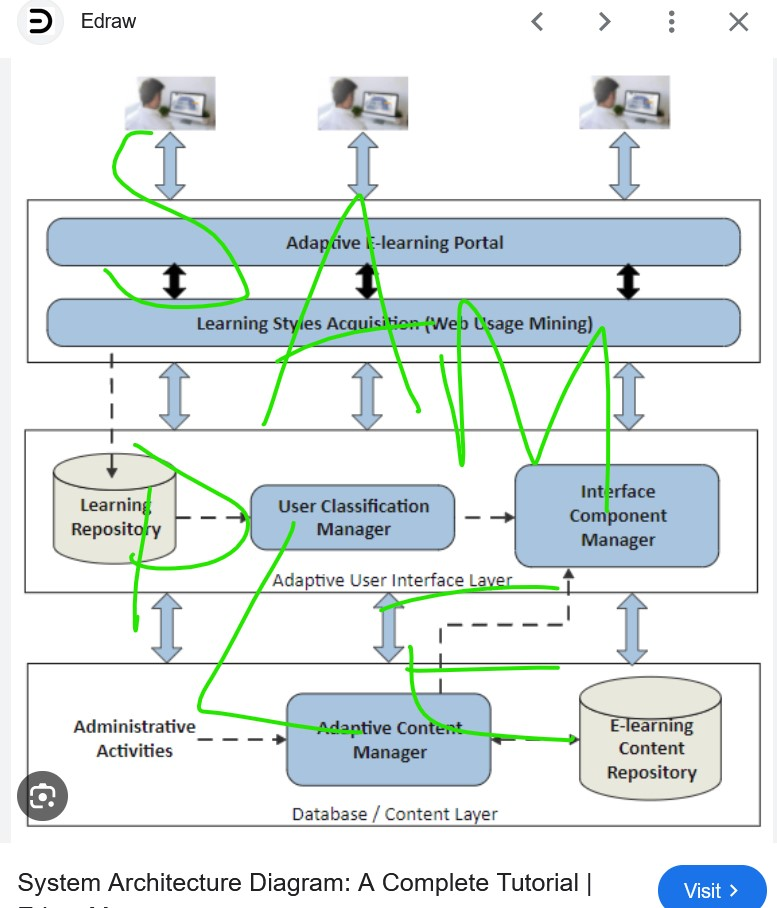
\includegraphics[width=1\textwidth]{figures/results/system_architecture.jpg}
%     \caption{Overall System Performance Analysis}
%     \label{fig:systemPerformance}
% \end{figure}

% Example listing (such as text output from console)
% \begin{figure}[H]
%     \begin{lstlisting}[style=cstyle]
%     // Environmental test results
%     // Temperature, ambient light, and vibration effects
%     \end{lstlisting}
%     \caption{Environmental Testing Results}
%     \label{lst:EnvironmentalTests1}
%     \end{figure}



% LATEX flowchart
% Include a flowchart
% \begin{figure}[H]
%     \centering
%     \scalebox{0.8}{ % Scale to 80% of original size
%         % try generating flowcharts as svg in Claude 
% and edit with inkscape instead of this.
% but claude did generate this one so might 
% be useful too but you can't easily make
% small repairs in inkscape


% CNN Transfer Learning Flowchart - Compact Multi-Column Layout
% \begin{figure}[htbp]

\centering
\resizebox{\textwidth}{!}{ % Scale to fit width while maintaining aspect ratio
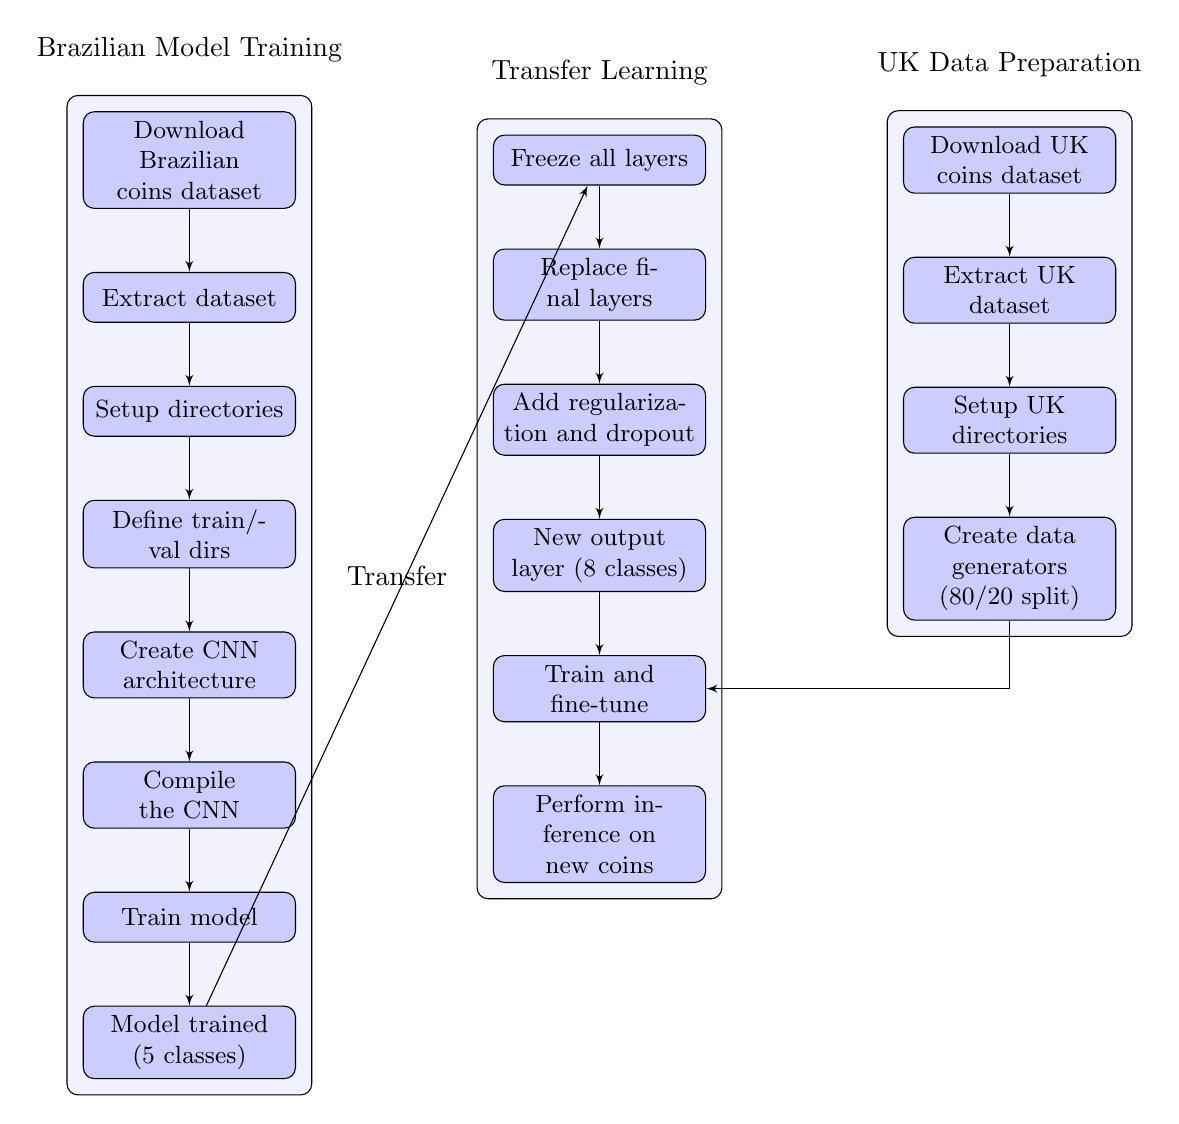
\begin{tikzpicture}[node distance=0.8cm and 1.5cm, auto]
    % Define a smaller block style
    \tikzset{
      block/.style = {rectangle, draw, fill=blue!20, 
                      text width=7em, text centered, rounded corners, minimum height=1.8em, font=\small},
    }
    
    % Brazilian model training - Column 1
    \node [block] (brazildata) {Download Brazilian coins dataset};
    \node [block, below=of brazildata] (extract) {Extract dataset};
    \node [block, below=of extract] (setup) {Setup directories};
    \node [block, below=of setup] (define) {Define train/val dirs};
    \node [block, below=of define] (create) {Create CNN architecture};
    \node [block, below=of create] (compile) {Compile the CNN};
    \node [block, below=of compile] (train) {Train model};
    \node [block, below=of train] (trained) {Model trained (5 classes)};
    
    % Transfer learning - Column 2 (Middle)
    \node [block, right=2.5cm of brazildata] (freeze) {Freeze all layers};
    \node [block, below=of freeze] (replace) {Replace final layers};
    \node [block, below=of replace] (add) {Add regularization and dropout};
    \node [block, below=of add] (output) {New output layer (8 classes)};
    \node [block, below=of output] (finaltrain) {Train and fine-tune};
    \node [block, below=of finaltrain] (inference) {Perform inference on new coins};
    
    % UK data preparation - Column 3 (Right)
    \node [block, right=2.5cm of freeze] (ukdata) {Download UK coins dataset};
    \node [block, below=of ukdata] (ukextract) {Extract UK dataset};
    \node [block, below=of ukextract] (uksetup) {Setup UK directories};
    \node [block, below=of uksetup] (ukgen) {Create data generators (80/20 split)};
    
    % Connect all nodes with arrows
    \path [line] (brazildata) -- (extract);
    \path [line] (extract) -- (setup);
    \path [line] (setup) -- (define);
    \path [line] (define) -- (create);
    \path [line] (create) -- (compile);
    \path [line] (compile) -- (train);
    \path [line] (train) -- (trained);
    
    \path [line] (ukdata) -- (ukextract);
    \path [line] (ukextract) -- (uksetup);
    \path [line] (uksetup) -- (ukgen);
    
    % Connect the columns
    \path [line] (trained) -- node[midway, above] {Transfer} (freeze);
    \path [line] (ukgen) |- (finaltrain);
    
    % Connect middle column
    \path [line] (freeze) -- (replace);
    \path [line] (replace) -- (add);
    \path [line] (add) -- (output);
    \path [line] (output) -- (finaltrain);
    \path [line] (finaltrain) -- (inference);
    
    % Group boxes to show different stages with smaller padding
    \begin{pgfonlayer}{background}
        \node[group={[yshift=0.3cm]above:Brazilian Model Training}, fit={(brazildata) (extract) (setup) (define) (create) (compile) (train) (trained)}, inner sep=0.2cm] {};
        \node[group={[yshift=0.3cm]above:UK Data Preparation}, fit={(ukdata) (ukextract) (uksetup) (ukgen)}, inner sep=0.2cm] {};
        \node[group={[yshift=0.3cm]above:Transfer Learning}, fit={(freeze) (replace) (add) (output) (finaltrain) (inference)}, inner sep=0.2cm] {};
    \end{pgfonlayer}
\end{tikzpicture}
}
% \caption{CNN Transfer Learning Flowchart: Brazilian to UK Coins}
% \label{fig:cnn-flowchart}
% \end{figure}
%     }
%     \caption{System Design Overview Flowchart}
%     \label{fig:decriptiveLabel3} % descriptive to call in text with \ref{fig:decriptiveLabel}
% \end{figure}
% PhotodiodeAngularResponse.tex
% \section{Photodiode Angular Response}
% This section discusses the results of the response of the solar sensor to angular changes of the light source.








% Example figure jpg
%
% \begin{figure}[htb]
%     \centering
%     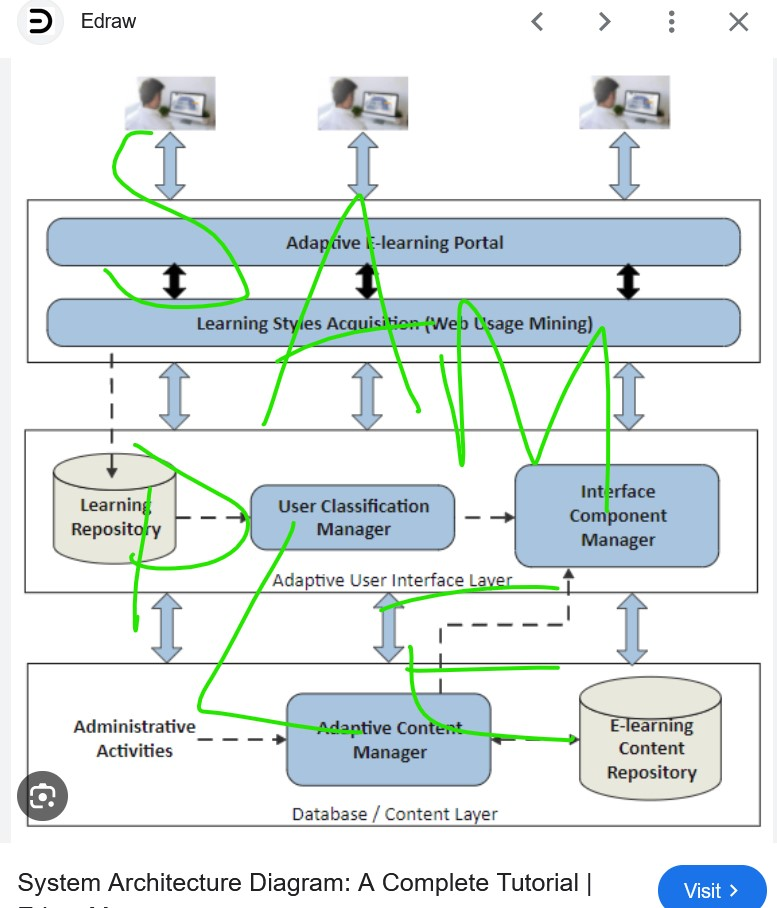
\includegraphics[width=1\textwidth]{figures/results/system_architecture.jpg}
%     \caption{Overall System Performance Analysis}
%     \label{fig:systemPerformance}
% \end{figure}

% Example listing (such as text output from console)
% \begin{figure}[H]
%     \begin{lstlisting}[style=cstyle]
%     // Environmental test results
%     // Temperature, ambient light, and vibration effects
%     \end{lstlisting}
%     \caption{Environmental Testing Results}
%     \label{lst:EnvironmentalTests1}
%     \end{figure}



% LATEX flowchar
% Include a flowchart
% \begin{figure}[H]
%     \centering
%     \scalebox{0.8}{ % Scale to 80% of original size
%         % try generating flowcharts as svg in Claude 
% and edit with inkscape instead of this.
% but claude did generate this one so might 
% be useful too but you can't easily make
% small repairs in inkscape


% CNN Transfer Learning Flowchart - Compact Multi-Column Layout
% \begin{figure}[htbp]

\centering
\resizebox{\textwidth}{!}{ % Scale to fit width while maintaining aspect ratio
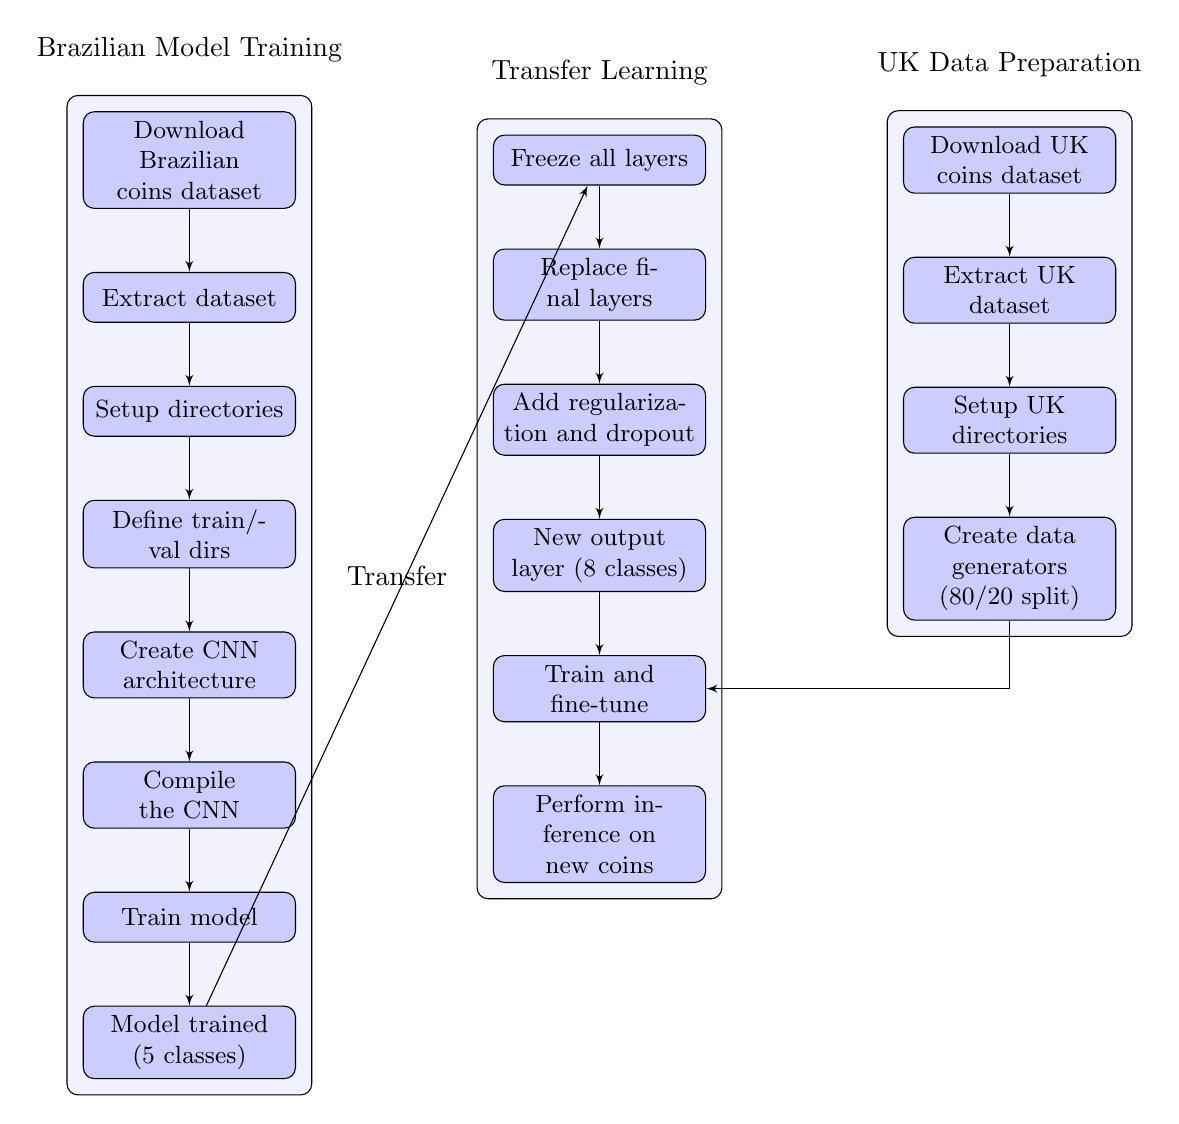
\begin{tikzpicture}[node distance=0.8cm and 1.5cm, auto]
    % Define a smaller block style
    \tikzset{
      block/.style = {rectangle, draw, fill=blue!20, 
                      text width=7em, text centered, rounded corners, minimum height=1.8em, font=\small},
    }
    
    % Brazilian model training - Column 1
    \node [block] (brazildata) {Download Brazilian coins dataset};
    \node [block, below=of brazildata] (extract) {Extract dataset};
    \node [block, below=of extract] (setup) {Setup directories};
    \node [block, below=of setup] (define) {Define train/val dirs};
    \node [block, below=of define] (create) {Create CNN architecture};
    \node [block, below=of create] (compile) {Compile the CNN};
    \node [block, below=of compile] (train) {Train model};
    \node [block, below=of train] (trained) {Model trained (5 classes)};
    
    % Transfer learning - Column 2 (Middle)
    \node [block, right=2.5cm of brazildata] (freeze) {Freeze all layers};
    \node [block, below=of freeze] (replace) {Replace final layers};
    \node [block, below=of replace] (add) {Add regularization and dropout};
    \node [block, below=of add] (output) {New output layer (8 classes)};
    \node [block, below=of output] (finaltrain) {Train and fine-tune};
    \node [block, below=of finaltrain] (inference) {Perform inference on new coins};
    
    % UK data preparation - Column 3 (Right)
    \node [block, right=2.5cm of freeze] (ukdata) {Download UK coins dataset};
    \node [block, below=of ukdata] (ukextract) {Extract UK dataset};
    \node [block, below=of ukextract] (uksetup) {Setup UK directories};
    \node [block, below=of uksetup] (ukgen) {Create data generators (80/20 split)};
    
    % Connect all nodes with arrows
    \path [line] (brazildata) -- (extract);
    \path [line] (extract) -- (setup);
    \path [line] (setup) -- (define);
    \path [line] (define) -- (create);
    \path [line] (create) -- (compile);
    \path [line] (compile) -- (train);
    \path [line] (train) -- (trained);
    
    \path [line] (ukdata) -- (ukextract);
    \path [line] (ukextract) -- (uksetup);
    \path [line] (uksetup) -- (ukgen);
    
    % Connect the columns
    \path [line] (trained) -- node[midway, above] {Transfer} (freeze);
    \path [line] (ukgen) |- (finaltrain);
    
    % Connect middle column
    \path [line] (freeze) -- (replace);
    \path [line] (replace) -- (add);
    \path [line] (add) -- (output);
    \path [line] (output) -- (finaltrain);
    \path [line] (finaltrain) -- (inference);
    
    % Group boxes to show different stages with smaller padding
    \begin{pgfonlayer}{background}
        \node[group={[yshift=0.3cm]above:Brazilian Model Training}, fit={(brazildata) (extract) (setup) (define) (create) (compile) (train) (trained)}, inner sep=0.2cm] {};
        \node[group={[yshift=0.3cm]above:UK Data Preparation}, fit={(ukdata) (ukextract) (uksetup) (ukgen)}, inner sep=0.2cm] {};
        \node[group={[yshift=0.3cm]above:Transfer Learning}, fit={(freeze) (replace) (add) (output) (finaltrain) (inference)}, inner sep=0.2cm] {};
    \end{pgfonlayer}
\end{tikzpicture}
}
% \caption{CNN Transfer Learning Flowchart: Brazilian to UK Coins}
% \label{fig:cnn-flowchart}
% \end{figure}
%     }
%     \caption{System Design Overview Flowchart}
%     \label{fig:decriptiveLabel3} % descriptive to call in text with \ref{fig:decriptiveLabel}
% \end{figure}
% EnclosureEffectiveness.tex
\section{Enclosure Effectiveness}
The final design of the enclosure is shown in Figure~\ref{fig:CADFinal}.
 The enclosure was designed and modified throughout its various iterations to be lightweight and portable, while still providing adequate protection for the internal components. 
 The design also allowed for easy access to the internal components for maintenance and troubleshooting.
 The enclosure was deemed a successful design as it met the requirements of being a stable and portable platform for the internal components, as in the Photodiode array.
 Problems with previous designs were addressed in the final design iteration, such as the need for a easier access to the anode and cathode connections of the photodiode array, which was achieved by using a removable cover, the rail-lock system, for the enclosure.
 This system allowed for the photodiode array to be easily mounted and secured into position.
 This system also allowed for the height of the enclosure to be adjusted so that surface that mounted the glass and the aperture was at a suitable height for when it was in use with the RED testbench.


% % Include a flowchart
% \begin{figure}[H]
%     \centering
%     \scalebox{0.8}{ % Scale to 80% of original size
%         % try generating flowcharts as svg in Claude 
% and edit with inkscape instead of this.
% but claude did generate this one so might 
% be useful too but you can't easily make
% small repairs in inkscape


% CNN Transfer Learning Flowchart - Compact Multi-Column Layout
% \begin{figure}[htbp]

\centering
\resizebox{\textwidth}{!}{ % Scale to fit width while maintaining aspect ratio
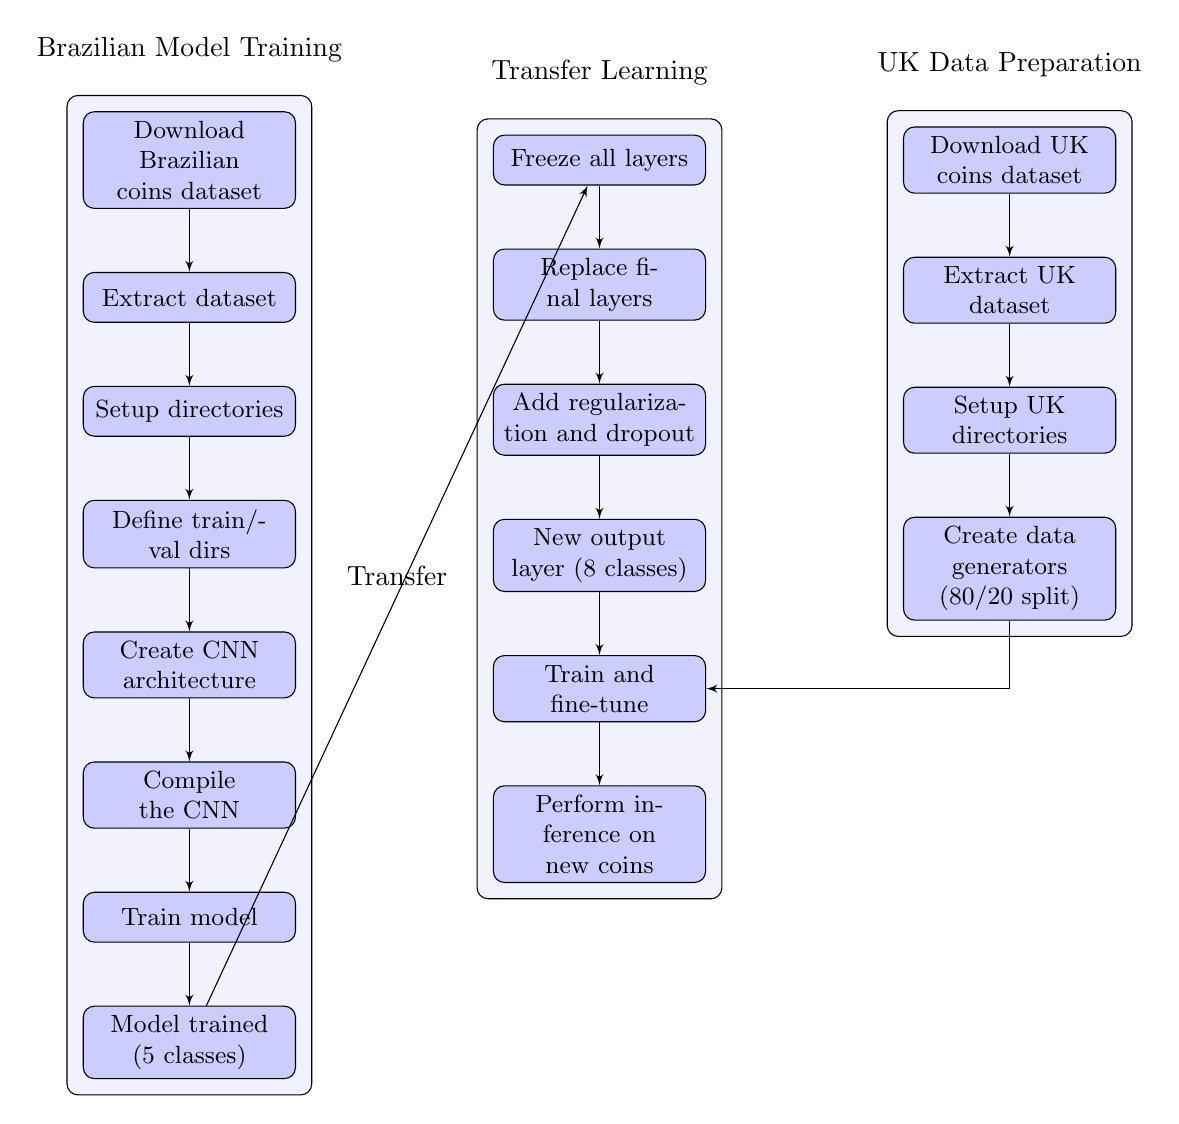
\begin{tikzpicture}[node distance=0.8cm and 1.5cm, auto]
    % Define a smaller block style
    \tikzset{
      block/.style = {rectangle, draw, fill=blue!20, 
                      text width=7em, text centered, rounded corners, minimum height=1.8em, font=\small},
    }
    
    % Brazilian model training - Column 1
    \node [block] (brazildata) {Download Brazilian coins dataset};
    \node [block, below=of brazildata] (extract) {Extract dataset};
    \node [block, below=of extract] (setup) {Setup directories};
    \node [block, below=of setup] (define) {Define train/val dirs};
    \node [block, below=of define] (create) {Create CNN architecture};
    \node [block, below=of create] (compile) {Compile the CNN};
    \node [block, below=of compile] (train) {Train model};
    \node [block, below=of train] (trained) {Model trained (5 classes)};
    
    % Transfer learning - Column 2 (Middle)
    \node [block, right=2.5cm of brazildata] (freeze) {Freeze all layers};
    \node [block, below=of freeze] (replace) {Replace final layers};
    \node [block, below=of replace] (add) {Add regularization and dropout};
    \node [block, below=of add] (output) {New output layer (8 classes)};
    \node [block, below=of output] (finaltrain) {Train and fine-tune};
    \node [block, below=of finaltrain] (inference) {Perform inference on new coins};
    
    % UK data preparation - Column 3 (Right)
    \node [block, right=2.5cm of freeze] (ukdata) {Download UK coins dataset};
    \node [block, below=of ukdata] (ukextract) {Extract UK dataset};
    \node [block, below=of ukextract] (uksetup) {Setup UK directories};
    \node [block, below=of uksetup] (ukgen) {Create data generators (80/20 split)};
    
    % Connect all nodes with arrows
    \path [line] (brazildata) -- (extract);
    \path [line] (extract) -- (setup);
    \path [line] (setup) -- (define);
    \path [line] (define) -- (create);
    \path [line] (create) -- (compile);
    \path [line] (compile) -- (train);
    \path [line] (train) -- (trained);
    
    \path [line] (ukdata) -- (ukextract);
    \path [line] (ukextract) -- (uksetup);
    \path [line] (uksetup) -- (ukgen);
    
    % Connect the columns
    \path [line] (trained) -- node[midway, above] {Transfer} (freeze);
    \path [line] (ukgen) |- (finaltrain);
    
    % Connect middle column
    \path [line] (freeze) -- (replace);
    \path [line] (replace) -- (add);
    \path [line] (add) -- (output);
    \path [line] (output) -- (finaltrain);
    \path [line] (finaltrain) -- (inference);
    
    % Group boxes to show different stages with smaller padding
    \begin{pgfonlayer}{background}
        \node[group={[yshift=0.3cm]above:Brazilian Model Training}, fit={(brazildata) (extract) (setup) (define) (create) (compile) (train) (trained)}, inner sep=0.2cm] {};
        \node[group={[yshift=0.3cm]above:UK Data Preparation}, fit={(ukdata) (ukextract) (uksetup) (ukgen)}, inner sep=0.2cm] {};
        \node[group={[yshift=0.3cm]above:Transfer Learning}, fit={(freeze) (replace) (add) (output) (finaltrain) (inference)}, inner sep=0.2cm] {};
    \end{pgfonlayer}
\end{tikzpicture}
}
% \caption{CNN Transfer Learning Flowchart: Brazilian to UK Coins}
% \label{fig:cnn-flowchart}
% \end{figure}
%     }
%     \caption{System Design Overview Flowchart}
%     \label{fig:decriptiveLabel5} % descriptive to call in text with \ref{fig:decriptiveLabel}
% \end{figure}

% \subsection{Functional Requirements}
% % Your content here

% \subsection{Design Approach}
% % Your content here

% \subsection{System Architecture}
% As shown in Figure~\ref{fig:decriptiveLabel5} the system architecture consists of various components.

% \begin{lstlisting}[style=cstyle, caption=System Architecture Code Example, label=lst:SystemArchitecture4]
% # Your code here
% \end{lstlisting}

% \begin{figure}[htbp] %h-ere t-op b-ottom p-page (separte) -good to allow all htbp to give the compiler more options
%     \centering
%     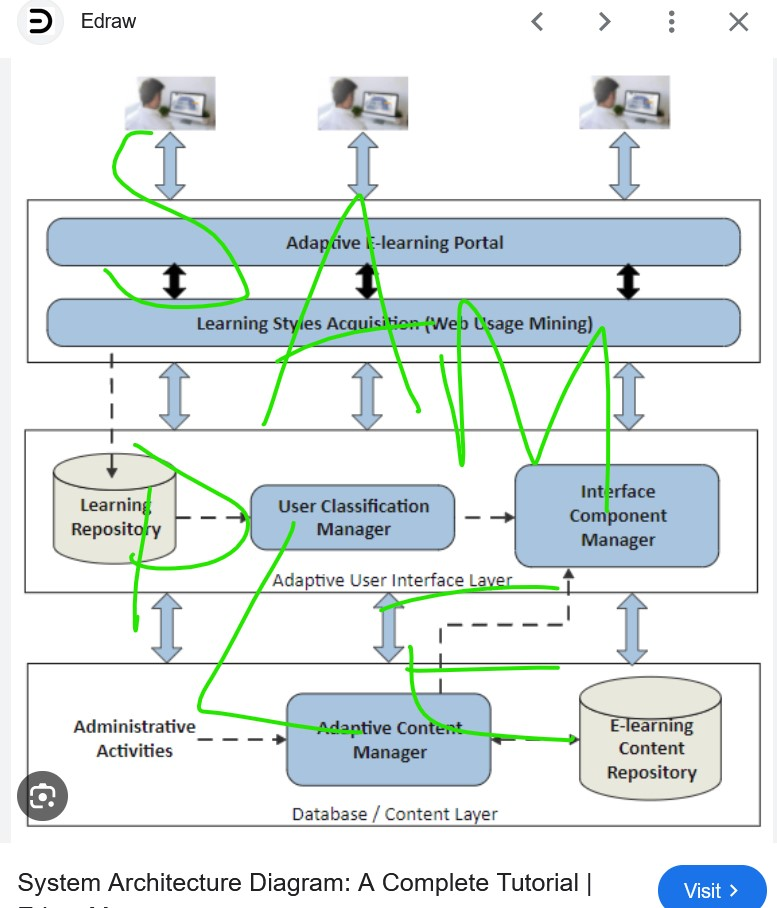
\includegraphics[width=0.6\textwidth]{figures/results/system_architecture.jpg}
%     \caption{System Architecture Diagram}
%     \label{fig:system-architecture22}
% \end{figure}
% DataAcquisitionSystemEvaluation.tex
\section{\acf{DAQ} System Evaluation}
The \ac{DAQ} was considered a success, it was able to take recordings in realtime of all four photodiodes and send them to a computer for post-processing. In it's final design the overal system that included the Python script as well as the Arduino, was able to perform it's task of generating both data in csv format that allowed comparison with simulated input, as well as the addition of noise filtering. % maybe add \ref to figures with graph 

% % Include a flowchart
% \begin{figure}[H]
%     \centering
%     \scalebox{0.8}{ % Scale to 80% of original size
%         % try generating flowcharts as svg in Claude 
% and edit with inkscape instead of this.
% but claude did generate this one so might 
% be useful too but you can't easily make
% small repairs in inkscape


% CNN Transfer Learning Flowchart - Compact Multi-Column Layout
% \begin{figure}[htbp]

\centering
\resizebox{\textwidth}{!}{ % Scale to fit width while maintaining aspect ratio
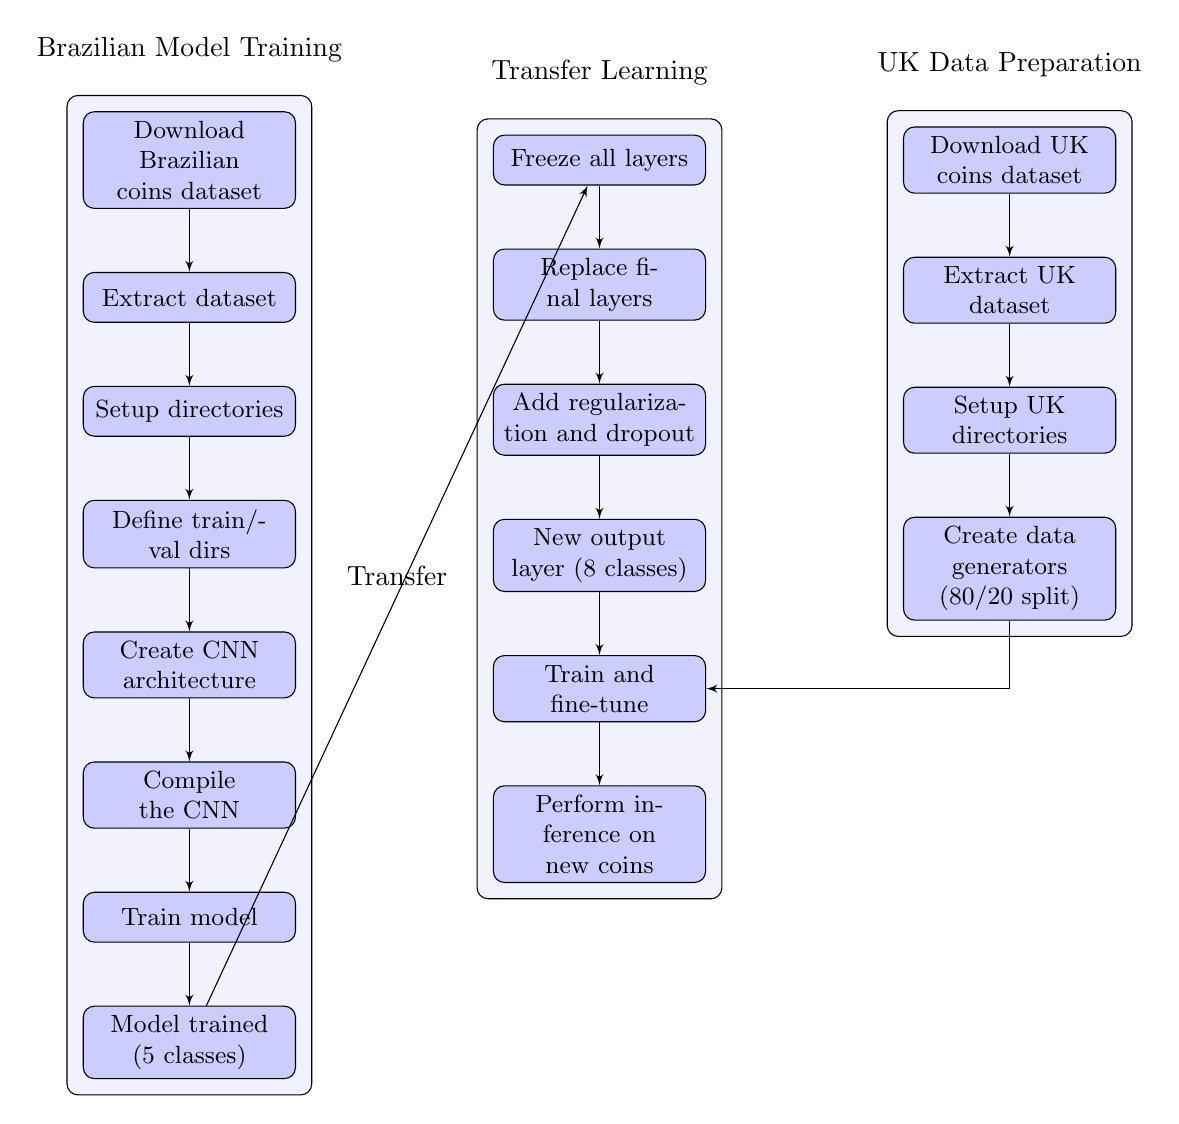
\begin{tikzpicture}[node distance=0.8cm and 1.5cm, auto]
    % Define a smaller block style
    \tikzset{
      block/.style = {rectangle, draw, fill=blue!20, 
                      text width=7em, text centered, rounded corners, minimum height=1.8em, font=\small},
    }
    
    % Brazilian model training - Column 1
    \node [block] (brazildata) {Download Brazilian coins dataset};
    \node [block, below=of brazildata] (extract) {Extract dataset};
    \node [block, below=of extract] (setup) {Setup directories};
    \node [block, below=of setup] (define) {Define train/val dirs};
    \node [block, below=of define] (create) {Create CNN architecture};
    \node [block, below=of create] (compile) {Compile the CNN};
    \node [block, below=of compile] (train) {Train model};
    \node [block, below=of train] (trained) {Model trained (5 classes)};
    
    % Transfer learning - Column 2 (Middle)
    \node [block, right=2.5cm of brazildata] (freeze) {Freeze all layers};
    \node [block, below=of freeze] (replace) {Replace final layers};
    \node [block, below=of replace] (add) {Add regularization and dropout};
    \node [block, below=of add] (output) {New output layer (8 classes)};
    \node [block, below=of output] (finaltrain) {Train and fine-tune};
    \node [block, below=of finaltrain] (inference) {Perform inference on new coins};
    
    % UK data preparation - Column 3 (Right)
    \node [block, right=2.5cm of freeze] (ukdata) {Download UK coins dataset};
    \node [block, below=of ukdata] (ukextract) {Extract UK dataset};
    \node [block, below=of ukextract] (uksetup) {Setup UK directories};
    \node [block, below=of uksetup] (ukgen) {Create data generators (80/20 split)};
    
    % Connect all nodes with arrows
    \path [line] (brazildata) -- (extract);
    \path [line] (extract) -- (setup);
    \path [line] (setup) -- (define);
    \path [line] (define) -- (create);
    \path [line] (create) -- (compile);
    \path [line] (compile) -- (train);
    \path [line] (train) -- (trained);
    
    \path [line] (ukdata) -- (ukextract);
    \path [line] (ukextract) -- (uksetup);
    \path [line] (uksetup) -- (ukgen);
    
    % Connect the columns
    \path [line] (trained) -- node[midway, above] {Transfer} (freeze);
    \path [line] (ukgen) |- (finaltrain);
    
    % Connect middle column
    \path [line] (freeze) -- (replace);
    \path [line] (replace) -- (add);
    \path [line] (add) -- (output);
    \path [line] (output) -- (finaltrain);
    \path [line] (finaltrain) -- (inference);
    
    % Group boxes to show different stages with smaller padding
    \begin{pgfonlayer}{background}
        \node[group={[yshift=0.3cm]above:Brazilian Model Training}, fit={(brazildata) (extract) (setup) (define) (create) (compile) (train) (trained)}, inner sep=0.2cm] {};
        \node[group={[yshift=0.3cm]above:UK Data Preparation}, fit={(ukdata) (ukextract) (uksetup) (ukgen)}, inner sep=0.2cm] {};
        \node[group={[yshift=0.3cm]above:Transfer Learning}, fit={(freeze) (replace) (add) (output) (finaltrain) (inference)}, inner sep=0.2cm] {};
    \end{pgfonlayer}
\end{tikzpicture}
}
% \caption{CNN Transfer Learning Flowchart: Brazilian to UK Coins}
% \label{fig:cnn-flowchart}
% \end{figure}
%     }
%     \caption{System Design Overview Flowchart}
%     \label{fig:decriptiveLabel6} % descriptive to call in text with \ref{fig:decriptiveLabel}
% \end{figure}

% \subsection{Functional Requirements}
% % Your content here

% \subsection{Design Approach}
% % Your content here

% \subsection{System Architecture}
% As shown in Figure~\ref{fig:decriptiveLabel6} the system architecture consists of various components.

% \begin{lstlisting}[style=cstyle, caption=System Architecture Code Example, label=lst:SystemArchitecture5]
% # Your code here
% \end{lstlisting}

% \begin{figure}[htbp] %h-ere t-op b-ottom p-page (separte) -good to allow all htbp to give the compiler more options
%     \centering
%     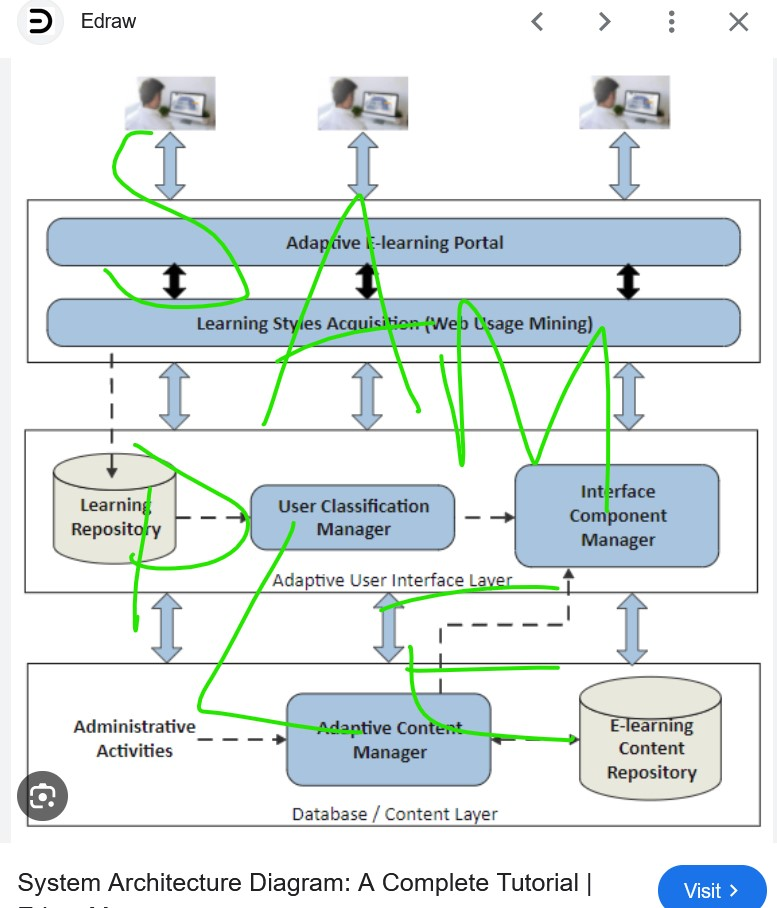
\includegraphics[width=0.6\textwidth]{figures/results/system_architecture.jpg}
%     \caption{System Architecture Diagram}
%     \label{fig:system-architecture21}
% \end{figure}
% % SystemPerformanceAnalysis.tex
\section{System Performance Analysis}

\subsection{Operational Constraints Identified}
% Your content here

\subsection{Environmental Factors Impact}
% Your content here



\subsection{System Stability and Repeatability}
% Your content here



\subsection{Recommendations for Improvement}
% Your content here



% Example figure jpg
%
% \begin{figure}[htb]
%     \centering
%     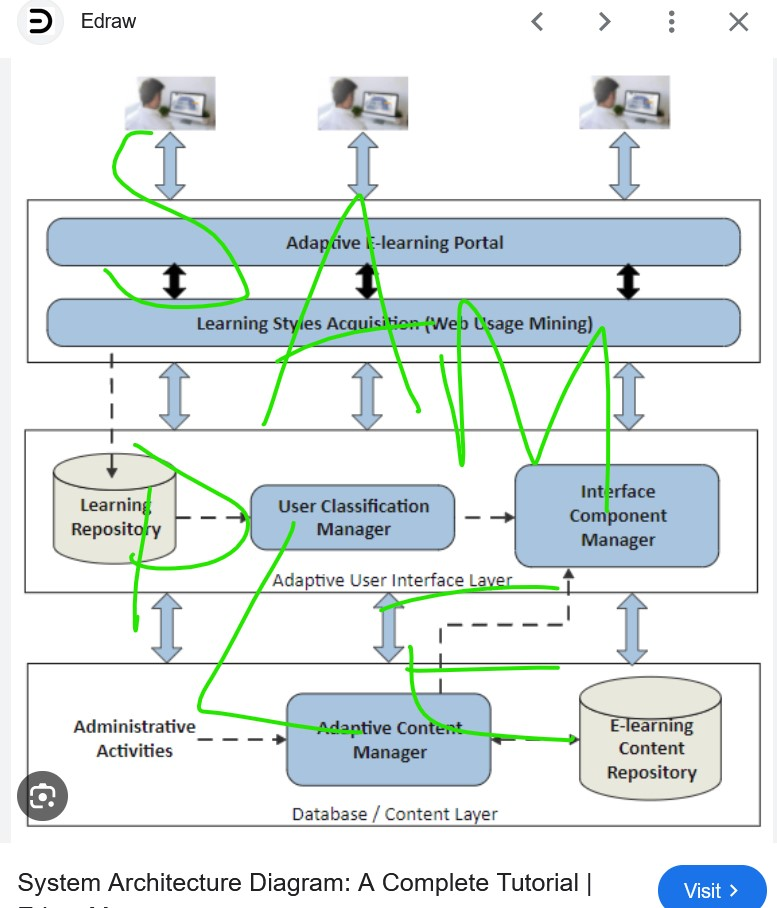
\includegraphics[width=1\textwidth]{figures/results/system_architecture.jpg}
%     \caption{Overall System Performance Analysis}
%     \label{fig:systemPerformance}
% \end{figure}

% Example listing (such as text output from console)
% \begin{figure}[H]
%     \begin{lstlisting}[style=cstyle]
%     // Environmental test results
%     // Temperature, ambient light, and vibration effects
%     \end{lstlisting}
%     \caption{Environmental Testing Results}
%     \label{lst:EnvironmentalTests1}
%     \end{figure}
% PrototypeComparison.tex
\section{Comparative Analysis}

To assess the accuracy of the developed simulation model, results from a full simulation run were compared against experimental data collected using the same sensor topology and an equivalent arc motion sequence.

Figure~\ref{fig:Model and Physical Results Comparison} presents a side-by-side comparison:
\begin{itemize}
    \item \textbf{Left:} Simulated illumination per sensor, expressed as the percentage of total emitted rays that intersected with each sensor area, plotted against the arc rotation angle.
    \item \textbf{Right:} Experimentally measured voltages from each physical sensor during the emitter's arc sweep. Signals have been filtered to reduce noise and highlight the response envelope.
\end{itemize}
\subsection*{Key Observations}
\begin{enumerate}
    \item \textbf{Overall Response Pattern:} Both plots show a clear progression of peak response across the sensor array. Sensor A2 activates first, followed by A1, A0, and then A3, which is consistent with the expected sequence during the rotation.
    
    \item \textbf{Peak Alignment:} The positions of the peak responses in the simulated and experimental plots align closely, suggesting that the source plane's movement and orientation in the simulation accurately reflects the RED testbench's real process.

\end{enumerate}
 \begin{landscape}
    \begin{figure}[htbp] %h-ere t-op b-ottom p-page (separte) -good to allow all htbp to give the compiler more options
        \centering
        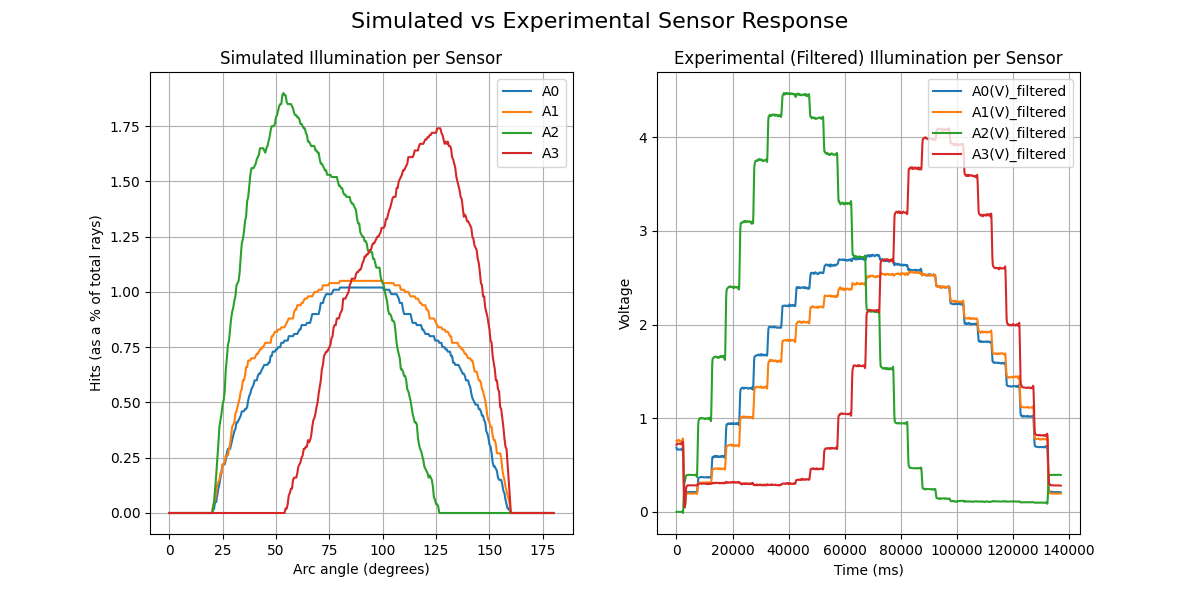
\includegraphics[width=1.4\textwidth]{chapters/results/images/Comparison_plot.png} % change {path}
        \caption{Model and Physical Results Comparison}       % change {caption}
        \label{fig:Model and Physical Results Comparison}            % change label - used for reference in text
    \end{figure}
 \end{landscape}

The simulation and hardware behave in the same way, sensors are gradually illuminated and fade out as expected. The simulation appears to be handling the geometry correctly, and the physical sensor design works as intended.


\subsection*{Interpretation}
This result provides strong validation for:
\begin{itemize}
    \item The geometric modelling of planes, areas, and ray emission in the simulation framework.
    \item The arc rotation logic, particularly the ``rigid arc'' strategy where the plane consistently faces the origin.
    \item The accuracy of the designed sensor layout and aperture configuration.
\end{itemize}


% Example figure jpg
%
% \begin{figure}[htb]
%     \centering
%     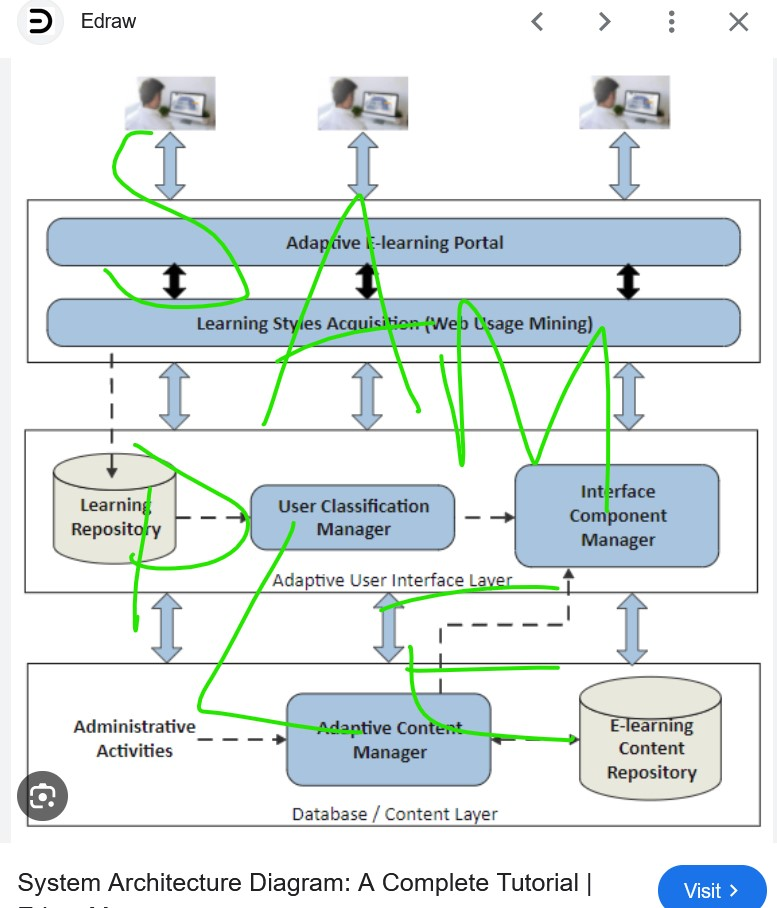
\includegraphics[width=1\textwidth]{figures/results/system_architecture.jpg}
%     \caption{Overall System Performance Analysis}
%     \label{fig:systemPerformance}
% \end{figure}

% Example listing (such as text output from console)
% \begin{figure}[H]
%     \begin{lstlisting}[style=cstyle]
%     // Environmental test results
%     // Temperature, ambient light, and vibration effects
%     \end{lstlisting}
%     \caption{Environmental Testing Results}
%     \label{lst:EnvironmentalTests1}
%     \end{figure}
% SystemLimitationsAndConsiderations.tex
\section{System Limitations And Considerations}
This section discusses the limitations and future work.
\subsection{\acf{RED} testbench limitations and impact}
The Renewable Energy Demonstrator (RED) device borrowed from the EPS team \cite{RefWorks:shopov2022renewable} proved to be valuable as a testbench for our project, but several limitations affected our ability to gather comprehensive data for accurate sun vector determination.
\subsubsection{Servo Motor Limitations}
There were at least two issues with the Servo Motors which reduced our ability to gether data:
\begin{itemize}
    \item Inablity to reach the target angles requested in code without phisical intervention, presumably due to insufficient torque or gearing issues.
    \item Control deadband did not allow us to gather a large enough sample (small-angle adjustment) to create a \ac{LUT} that would allow the prediction of light position by interpolation.
\end{itemize}

When attempting to move from 0\textdegree{} to 90\textdegree{}, for example, the servomotors would often stall, requiring manual assistance to ``help'' the arch reach the desired position. This introduced inconsistency in our testing methodology and required manual adjustment using protractors.

\subsubsection{Signal Interference Issues}

The \ac{RED}'s Power Supply interference made the signal very noisy. However due to the nature of the high frequency noise and low frequency signal, it meant that it was relativly easy to filter using the scipy.signal library \cite{RefWorks:butter}, detailed in Section \ref{LowPassFilter}. Further, arch position changing without pressing the button likely due to noise in the \ac{RED} from the Power Supply made testing slighlty more annoying, but it was not happening often enough to disrupt testing too much, it was considered an acceptable quirk.

\subsubsection{Impact on Look-Up Table development}

The most significant impact to the project caused by these issues with the \ac{RED} are that we were unable to generate a \ac{LUT} or a "Sensor Response Surface" plot using the prototype, as the angle precision from the arch was not good enough. Originally, our plan included:

\begin{itemize}
    \item Taking measurements at fine angular increments (every 5\textdegree{}) across the hemisphere
    \item Mapping between sensor readings and light source position
    \item Using said mapping to develop interpolation algorithms for positions between measured points
    \item Validating position determination accuracy across the sensor's field of view
\end{itemize}

The compbination of these limitations of the \ac{RED} testbench made it impractical to gather the comprehensive dataset required to fulfill these goals, as withouht a reliable dataset across the entire \ac{FOV} it is not possible to predict the location of light.
This limitations ultimatly directly affected the ability to detect the light position, and we could only take some readings and compare them to the simulated environment.

\subsection{Aperture placement accuracy}

Another big limitatino on accuracy of the readings will be the manually placed apertures. As shown earlier in Figure \ref{fig:aperturePhoto}, the apertures are far from perfectly in the middle. This will have a huge impact on the accuracy of the readings especially when compared to a simulated environment which have perfectly placed apertures. Howver, if we had been able to create a \ac{LUT} using the real measurements with aperture as-is, the results could have theoretically been used to read the location of light. Unfortunately, as stated above, that was also impossible due to the limitations of the testbench. These two main factors were the main cause of not being able to perform a calibration and perform actual readings to test the ability to read light locations. 

\subsection{Model Limitations and Future Work}
\begin{itemize}
    \item The vertical scale differs between plots figure~\ref{fig:Model and Physical Results Comparison}: simulated hits are relative percentages, while the experimental data reflects voltage. A calibration factor could be introduced in future to improve this correspondence.
    \item Minor asymmetries in the experimental data may arise from mechanical inaccuracies or misalignment, which are not currently modelled.
    \item Future improvements may incorporate ray divergence, non-ideal optics, or sensor sensitivity profiles to further refine realism.
\end{itemize}

% Your content here

% \subsection{}
% Your content here

% \subsection{}


% Example figure jpg
%
% \begin{figure}[htb]
%     \centering
%     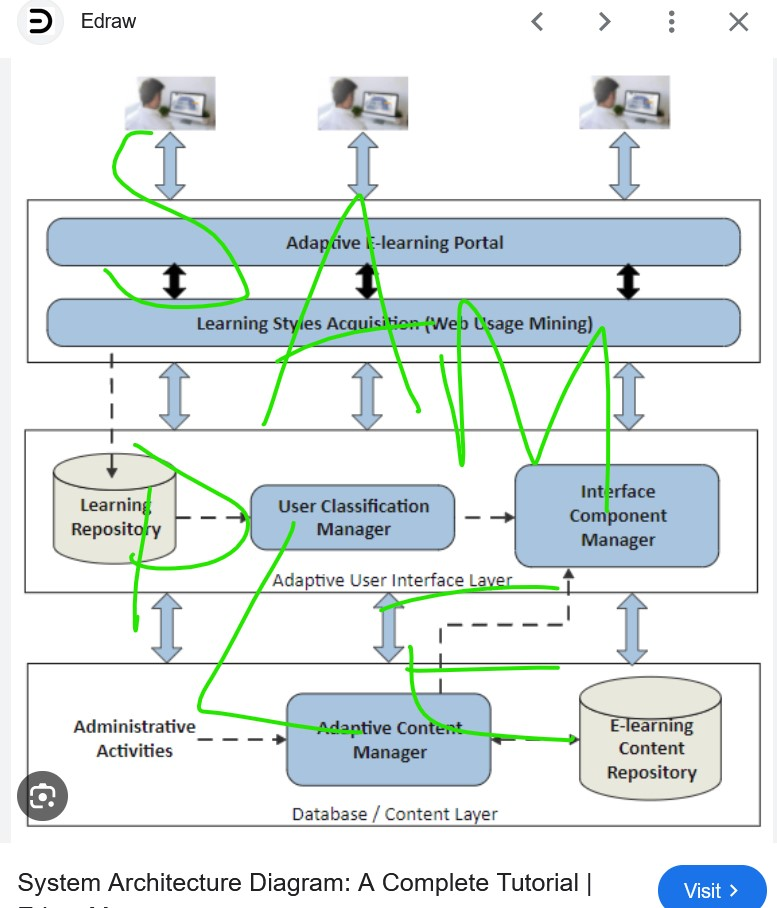
\includegraphics[width=1\textwidth]{figures/results/system_architecture.jpg}
%     \caption{Overall System Performance Analysis}
%     \label{fig:systemPerformance}
% \end{figure}

% Example listing (such as text output from console)
% \begin{figure}[H]
%     \begin{lstlisting}[style=cstyle]
%     // Environmental test results
%     // Temperature, ambient light, and vibration effects
%     \end{lstlisting}
%     \caption{Environmental Testing Results}
%     \label{lst:EnvironmentalTests1}
%     \end{figure}



% Example LATEX flowchart
% Include a flowchart
% \begin{figure}[H]
%     \centering
%     \scalebox{0.8}{ % Scale to 80% of original size
%         % try generating flowcharts as svg in Claude 
% and edit with inkscape instead of this.
% but claude did generate this one so might 
% be useful too but you can't easily make
% small repairs in inkscape


% CNN Transfer Learning Flowchart - Compact Multi-Column Layout
% \begin{figure}[htbp]

\centering
\resizebox{\textwidth}{!}{ % Scale to fit width while maintaining aspect ratio
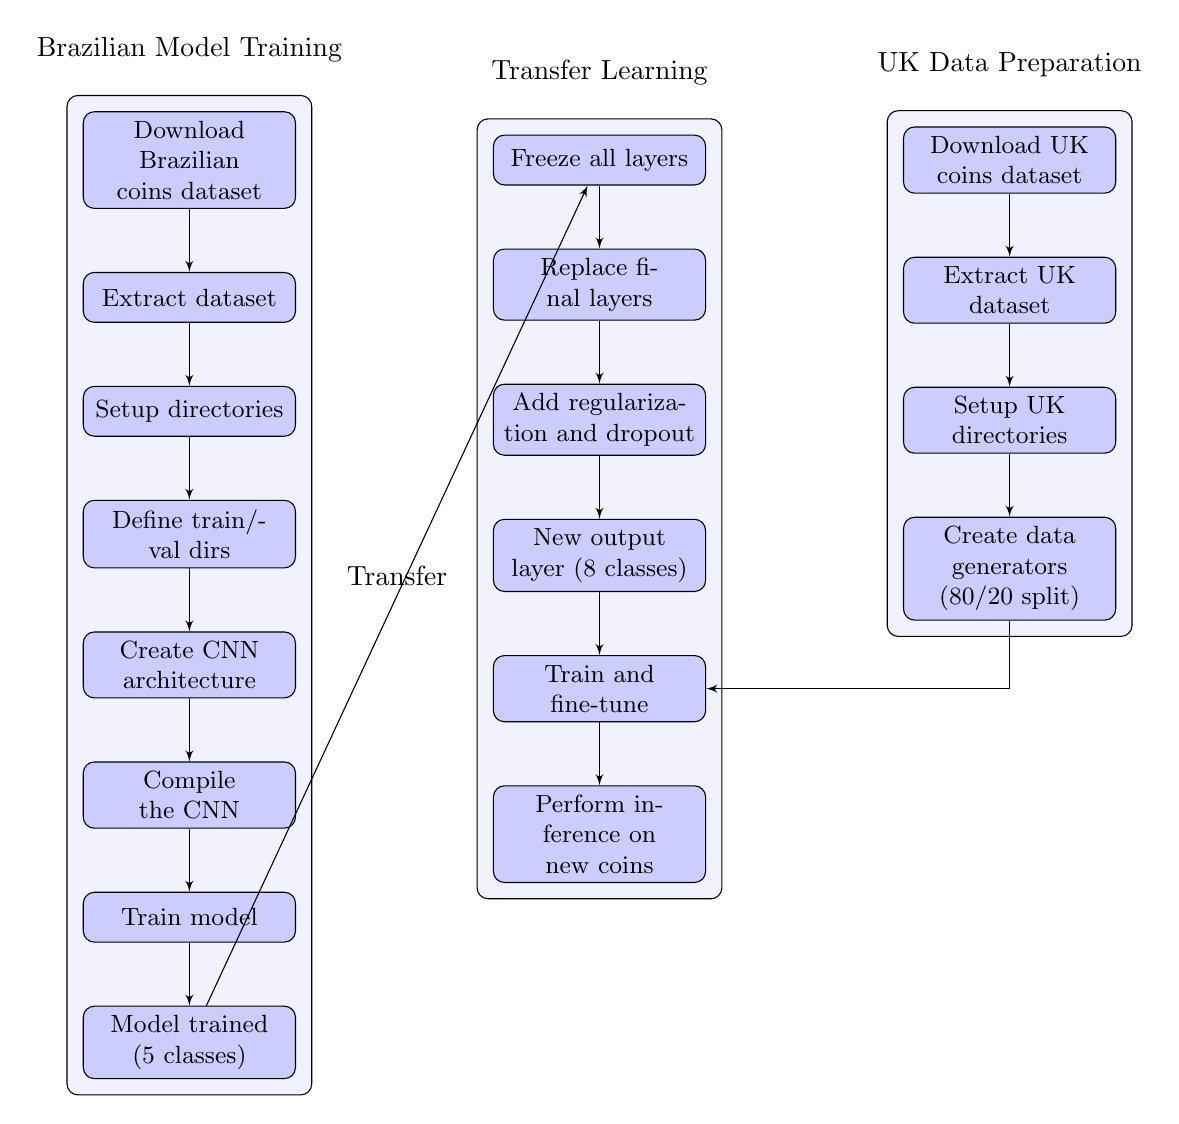
\begin{tikzpicture}[node distance=0.8cm and 1.5cm, auto]
    % Define a smaller block style
    \tikzset{
      block/.style = {rectangle, draw, fill=blue!20, 
                      text width=7em, text centered, rounded corners, minimum height=1.8em, font=\small},
    }
    
    % Brazilian model training - Column 1
    \node [block] (brazildata) {Download Brazilian coins dataset};
    \node [block, below=of brazildata] (extract) {Extract dataset};
    \node [block, below=of extract] (setup) {Setup directories};
    \node [block, below=of setup] (define) {Define train/val dirs};
    \node [block, below=of define] (create) {Create CNN architecture};
    \node [block, below=of create] (compile) {Compile the CNN};
    \node [block, below=of compile] (train) {Train model};
    \node [block, below=of train] (trained) {Model trained (5 classes)};
    
    % Transfer learning - Column 2 (Middle)
    \node [block, right=2.5cm of brazildata] (freeze) {Freeze all layers};
    \node [block, below=of freeze] (replace) {Replace final layers};
    \node [block, below=of replace] (add) {Add regularization and dropout};
    \node [block, below=of add] (output) {New output layer (8 classes)};
    \node [block, below=of output] (finaltrain) {Train and fine-tune};
    \node [block, below=of finaltrain] (inference) {Perform inference on new coins};
    
    % UK data preparation - Column 3 (Right)
    \node [block, right=2.5cm of freeze] (ukdata) {Download UK coins dataset};
    \node [block, below=of ukdata] (ukextract) {Extract UK dataset};
    \node [block, below=of ukextract] (uksetup) {Setup UK directories};
    \node [block, below=of uksetup] (ukgen) {Create data generators (80/20 split)};
    
    % Connect all nodes with arrows
    \path [line] (brazildata) -- (extract);
    \path [line] (extract) -- (setup);
    \path [line] (setup) -- (define);
    \path [line] (define) -- (create);
    \path [line] (create) -- (compile);
    \path [line] (compile) -- (train);
    \path [line] (train) -- (trained);
    
    \path [line] (ukdata) -- (ukextract);
    \path [line] (ukextract) -- (uksetup);
    \path [line] (uksetup) -- (ukgen);
    
    % Connect the columns
    \path [line] (trained) -- node[midway, above] {Transfer} (freeze);
    \path [line] (ukgen) |- (finaltrain);
    
    % Connect middle column
    \path [line] (freeze) -- (replace);
    \path [line] (replace) -- (add);
    \path [line] (add) -- (output);
    \path [line] (output) -- (finaltrain);
    \path [line] (finaltrain) -- (inference);
    
    % Group boxes to show different stages with smaller padding
    \begin{pgfonlayer}{background}
        \node[group={[yshift=0.3cm]above:Brazilian Model Training}, fit={(brazildata) (extract) (setup) (define) (create) (compile) (train) (trained)}, inner sep=0.2cm] {};
        \node[group={[yshift=0.3cm]above:UK Data Preparation}, fit={(ukdata) (ukextract) (uksetup) (ukgen)}, inner sep=0.2cm] {};
        \node[group={[yshift=0.3cm]above:Transfer Learning}, fit={(freeze) (replace) (add) (output) (finaltrain) (inference)}, inner sep=0.2cm] {};
    \end{pgfonlayer}
\end{tikzpicture}
}
% \caption{CNN Transfer Learning Flowchart: Brazilian to UK Coins}
% \label{fig:cnn-flowchart}
% \end{figure}
%     }
%     \caption{System Design Overview Flowchart}
%     \label{fig:decriptiveLabel4} % descriptive to call in text with \ref{fig:decriptiveLabel}
% \end{figure}
% Conclusions.tex
\chapter{Conclusions}

This project has successfully met its objective of developing a cost-effective and reliable analogue sun sensor system suitable for attitude determination in Low Earth Orbit (LEO) nanosatellite missions. Through the integration of hardware prototyping and software simulation, a robust methodology was established to evaluate the viability of photodiode-based sun sensing solutions.

A functional photodiode array was constructed, accompanied by a custom-designed signal conditioning circuit incorporating a transimpedance amplifier and post-amplification low-pass filtering. The system output was digitised using a Arduino-based data acquisition system, with post-processing conducted via Python to apply digital filtering and interpret results.

The software model, implemented in Python, and built on fundamental geometric principles, modelled ray-plane interactions using geometric approximation.  It features flexible configuration of sensor and aperture topologies, and supported visual and quantitative analysis of illumination results across a range of incident angles and positions. Conducting comparative analysis, between experimental (RED testbench) and simulated (Software model) data, validated the successful implementation of underlying principles and assumptions, by proving a strong correlation.

While the Renewable Energy Demonstrator (RED) testbench introduced some mechanical limitations, such as inconsistent servo performance and control noise, these were effectively mitigated through calibration, manual adjustments, and signal filtering techniques.

Ultimately, this project delivers a validated hybrid sun sensing system — combining practical prototyping with a software model.
% Your introduction content here
  
\chapter{Future Work}
Mention: methods to avoid detecting sun reflections off the moon and earth (such as light intensity or light source width if possible).

Unfortunately, there was no other easily available method of fabricating the apertures, such as having the apertures printed on glass with a fully opaque ink. Another method considered and attempted was to 3D print the apertures, but this would have resulted in the apertures having a thickness that would have changed the way the light enters, depending on the angle of the light.


% Bibliography 
\bibliographystyle{IEEEtran}
\KOMAoption{bibliography}{totoc}  % KOMA-Script way to add to ToC
\bibliography{bibliography/references}


% Appendix
\appendix
\chapter{Appendix - DAQ Code}
\section{Arduino DAQ full code}
\subsection{Arduino C++ Code}
\label{subsec:arduinoCppcode}
%%% ARDUINO CPP CODE
\begin{lstlisting}[style=cstyle, caption=C++ Code on Arduino, label=lst:arduinoCodeApp, language=C++]
    /*
    * Reads 4 analog inputs (0-5V) for recording_dur seconds
    * Streams data to PC while recording
    */
    // change to true to print debug messages on Serial Monitor
    // printing debug lines impacts transmission speed and messes csv
    //  do not leave on during measurements!
    bool debug = false;
  
    const int analogInputs[] = {A0, A1, A2, A3};
    
    
    // set up the global varialbes
    unsigned long start_time;
    const unsigned long recording_dur = 5000; // 25 seconds in milliseconds (ENSURE python code is greater than this)
    unsigned long last_sample_time = 0;
    const unsigned long min_samp_interval = 2; // Sample every 2ms (adjust for stability)
    bool recording = false;
    int sample_count = 0;
    
    void setup() {
      // serial communication at 115200 bps
      Serial.begin(115200);
      
      // Set pins as input
      for (int i = 0; i < 4; i++) {
        pinMode(analogInputs[i], INPUT);
      }
      
      // Optimize ADC for faster sampling
      // Set ADC prescaler to 16 (default is 128)
      //
      // Bit: 7:enable; 6: initiate a convertion 5: 
      //
      ADCSRA = (ADCSRA & 0xF8) | 0x04;
      
      // Wait for serial connection to establish
      delay(1000);
      
      // Send ready message
      Serial.println("ARDUINO_DAQ_READY");
    }
    
    void loop() {
      // Check if we received a command
      if (Serial.available() > 0) {
        String command = Serial.readStringUntil('\n');
        command.trim();
        
        if (command == "START") {
          if(debug) Serial.println("received START command");
  
          // Clear any remaining data in serial buffer
          while (Serial.available()) {
            Serial.read();
          }
          
          // Reset sample counter
          sample_count = 0;
          
          // Send header once
          Serial.println("Sample,Time(ms),A0(V),A1(V),A2(V),A3(V)");
          
          // Start recording
          recording = true;
          start_time = millis();
          last_sample_time = start_time;
          
          // Send confirmation
          Serial.println("RECORDING_STARTED");
        }
      }
      
      // If we're recording, collect and send data immediately
      if (recording) {
        if(debug) Serial.println("Recording!");
        unsigned long currentTime = millis();
        unsigned long elapsed_time = currentTime - start_time;
        
        // Check if we're still within the recording period
        if (elapsed_time <= recording_dur) {
          if(debug) Serial.println("elapsed time << duration");
          // Only sample at the specified interval
          if (currentTime - last_sample_time >= min_samp_interval) {
            last_sample_time = currentTime;
            
            // Increment sample counter
            sample_count++;
            
            // Start building the output string
            String data_string = String(sample_count) + "," + String(elapsed_time);
            
            // Multiplex through the four inputs sequentially
            for (int i = 0; i < 4; i++) {
              if(debug) Serial.println("reading input: " + String(i));
              int raw_value = analogRead(analogInputs[i]);
              float voltage = raw_value * (5.0 / 1023.0);
              data_string += "," + String(voltage, 3);
            }
            
            // Send the complete data string at once
            Serial.println(data_string);
          }
        }
        else {
          // End of recording
          recording = false;
          
          // Send notification that recording is complete
          Serial.println("RECORDING_COMPLETE");
          Serial.print("SAMPLES_COLLECTED:");
          Serial.println(sample_count);
          Serial.println("END_OF_DATA");
        }
      }
    }
  
\end{lstlisting}
%
%
%
%       ~~~~~~~~~~~~~~ PYTHON SERIAL RECEIVE APPENDIX ~~~~~~~~~~~                  %
%
%
\subsection{PC-side Python Serial Receive Script}
%%% Python Script
\begin{lstlisting}[style=pythonstyle, caption=Python Serial Receive Script, label=lst:pythonCodeApp, language=Python ]
    import serial
    import time
    import matplotlib.pyplot as plt
    import pandas as pd
    import os
    import numpy as np
    from scipy import signal
    
    def apply_lowpass_filter(data, fs):
        """Apply a 4-pole low-pass Butterworth filter with 5Hz cutoff"""
        cutoff_freq = 2.0
        filter_order = 4
        
        nyquist = 0.5 * fs
        normal_cutoff = cutoff_freq / nyquist
        # analog=False implies  bilinear Transformation
        b, a = signal.butter(filter_order, normal_cutoff, btype='low', analog=False)
        filtered_data = signal.filtfilt(b, a, data)
        
        return filtered_data
    
    # Load data from CSV, apply a 4-pole low-pass filter, and save the filtered data
    def filter_and_save_data(filename):
        
        # Read the CSV data to pandas DataFrame
        #  It knows what are the column names
        df = pd.read_csv(filename)
        
        # Clean the dataframe - convert all columns to numeric
        for col in df.columns:                  # v - write NaN where it can't convert to number (in teh data, not column names)
            df[col] = pd.to_numeric(df[col], errors='coerce')
    
        # remove rows with NaN (not a number)
        df = df.dropna()
        
        # Samples not at exact distance from each other
        # Calculate the sampling frequency (median of differences)
        # numpy.diff to get the difference between samples
        time_diffs = np.diff(df['Time(ms)'])
        # numpy.median to get the median
        median_time_diff = np.median(time_diffs)  # in milliseconds
        fs = 1000.0 / median_time_diff  # Convert to Hz
        
        # Filter each analog channel:
        # ID column head for each channel 
        analog_channels = ['A0(V)', 'A1(V)', 'A2(V)', 'A3(V)']
        # take each channel one at a time
        for channel in analog_channels:
            # if name maches a column name
            if channel in df.columns:
                # add a new column _filtered, and send the array containing all the raw values to 
                # have them filtered, and save them in the new _filtered column
                df[f"{channel}_filtered"] = apply_lowpass_filter(df[channel].values, fs)
        
        # Save the pandas Dataframe with filtered columns to a new CSV file
        filtered_filename = f"{os.path.splitext(filename)[0]}_filtered.csv"
        df.to_csv(filtered_filename, index=False)
        
        return filtered_filename
    
    #
    # Plot the DAQ data with original and filtered signals overlapped
    #
    def plot_data(filename):
        
        # Read the CSV data with pandas
        df = pd.read_csv(filename)
        
        # Initialize an empty list to store our analog channel names
        analog_channels = []
    
        # Look through all column names in the DataFrame
        for col in df.columns:
            # the column name starts with 'A'
            if col.startswith('A'):
                #  the column name ends with '(V)'
                if col.endswith('(V)'):
                    # the column name does NOT contain '_filtered'
                    if '_filtered' not in col:
                        # add this column name to our list
                        analog_channels.append(col)
        
        # Create color cycle for different channels
        colors = ['blue', 'green', 'red', 'purple']
        
        # Create a single plot with all channels overlapping
        plt.figure(figsize=(14, 8))
        
        # Plot original data (semi-transparent)
        for i, channel in enumerate(analog_channels):
            color = colors[i % len(colors)]
            plt.plot(df['Time(ms)'], df[channel], label=f'{channel} Original', 
                    linewidth=1.5, alpha=0.4, color=color, linestyle='-')
        
        # Plot filtered data (solid lines)
        for i, channel in enumerate(analog_channels):
            filtered_channel = f"{channel}_filtered"
            if filtered_channel in df.columns:
                color = colors[i % len(colors)]
                plt.plot(df['Time(ms)'], df[filtered_channel], label=f'{channel} Filtered', 
                        linewidth=2.5, color=color, linestyle='-')
        
        # Set the y-axis range from 0 to 5V
        plt.ylim(0, 5)
        
        # Add labels and title
        plt.xlabel('Time (ms)')
        plt.ylabel('Voltage (V)')
        plt.title('Arduino DAQ - 4-Channel Readings with 4-Pole 5Hz Low-Pass Filter')
        plt.legend()
        plt.grid(True)
            
        # Add data summary
        duration = df['Time(ms)'].max() - df['Time(ms)'].min()
        sample_count = len(df)
        sample_rate = sample_count/(duration/1000) if duration > 0 else 0
        
        info_text = f"Data summary:\n" \
                    f"Duration: {duration:.1f} ms\n" \
                    f"Samples: {sample_count}\n" \
                    f"Sample rate: {sample_rate:.1f} Hz\n" \
                    f"Filter: 4-pole Butterworth, 5Hz cutoff"
                    
        plt.figtext(0.02, 0.02, info_text, fontsize=10, 
                    bbox=dict(facecolor='white', alpha=0.8))
        
        # Save the plot
        plot_filename = f"{os.path.splitext(filename)[0]}_plot.png"
        plt.savefig(plot_filename, dpi=300, bbox_inches='tight')
        
        # Show the plot
        plt.tight_layout()
        plt.show()
    
    def main():
    
        # ASk if to plot or measure
        what_to_do = int(input("Record new measurement (1) or plot existing (2): "))
    
        # User selected to plot old csv
        if(what_to_do == 2):
            plot_data(input("Insert the name of the csv: "))
        
    
        # User selected to record new measurement
        elif(what_to_do == 1):
            # Use a default port (COM3 for Windows, modify as needed)
            default_port = "COM3"  # Change to match your system
            
            print(f"Using  port: {default_port}")
            
            # Configure serial port
            try:
                ser = serial.Serial(default_port, 115200, timeout=2)
                print("Connected to Arduino!")
            except serial.SerialException:
                print(f"Error: Could not open port {default_port}")
                print("Please modify the default_port variable in the script.")
                return
            
            time.sleep(2)  # Wait for Arduino to reset
            
            # Flush buffers
            ser.reset_input_buffer()
            ser.reset_output_buffer()
            
            # Wait for Arduino ready
            print("Waiting for Arduino to be ready...")
            ready = False
            timeout = time.time() + 10 # don't wait too long
            
            while not ready and time.time() < timeout:
                line = ser.readline().decode('utf-8', errors='ignore').strip()
                if line == "ARDUINO_DAQ_READY":
                    ready = True
                    print("Arduino is ready!")
            
            if not ready:
                print("Timed out waiting for Arduino. Make sure it's properly connected.")
                ser.close()
                return
            
            # Create a filename for this recording session
            filename = f"arduino_daq_data_{time.strftime('%Y%m%d_%H%M%S')}.csv"
            
            print(f"Starting data recording to {filename}...")
            print("Press Ctrl+C to stop if needed.")
            
            with open(filename, 'w', newline='') as file:
                # Send start command
                ser.write(b"START\n")
                
                recording = True
                data_lines = 0
                
                # Start time for timeout
                start_time = time.time()
                timeout_duration = 15  # seconds
                
                while recording and (time.time() - start_time) < timeout_duration:
                    if ser.in_waiting:
                        line = ser.readline().decode('utf-8', errors='ignore').strip()
                        
                        if "RECORDING_COMPLETE" in line:
                            recording = False
                            print("Recording complete!")
                        elif "END_OF_DATA" in line:
                            pass
                        elif line:
                            # Write the line to the file
                            file.write(line + '\n')
                            data_lines += 1
                            
                            # Show progress occasionally
                            if data_lines % 100 == 0:
                                print(f"Recorded {data_lines} data points...")
            
            # Close the serial port
            if ser.is_open:
                ser.close()
                print("Serial port closed.")
            
            print(f"Recorded {data_lines} lines of data.")
            
            # Process the data
            print("Applying filters to data...")
            filtered_filename = filter_and_save_data(filename)
            print(f"Filtered data saved to {filtered_filename}")
            
            print("Generating plot...")
            plot_data(filtered_filename)
            print("Done!")
            
        else:
            print("Wrong Choice. Goodbye!")
            exit()
    if __name__ == "__main__":
        try:
            main()
        except KeyboardInterrupt:
            print("\nProgram terminated by user.")
\end{lstlisting}

\section{Derivation of TIA Voltage Out}

% V out derivation
%
\begin{figure}[htbp] 
    \centering
    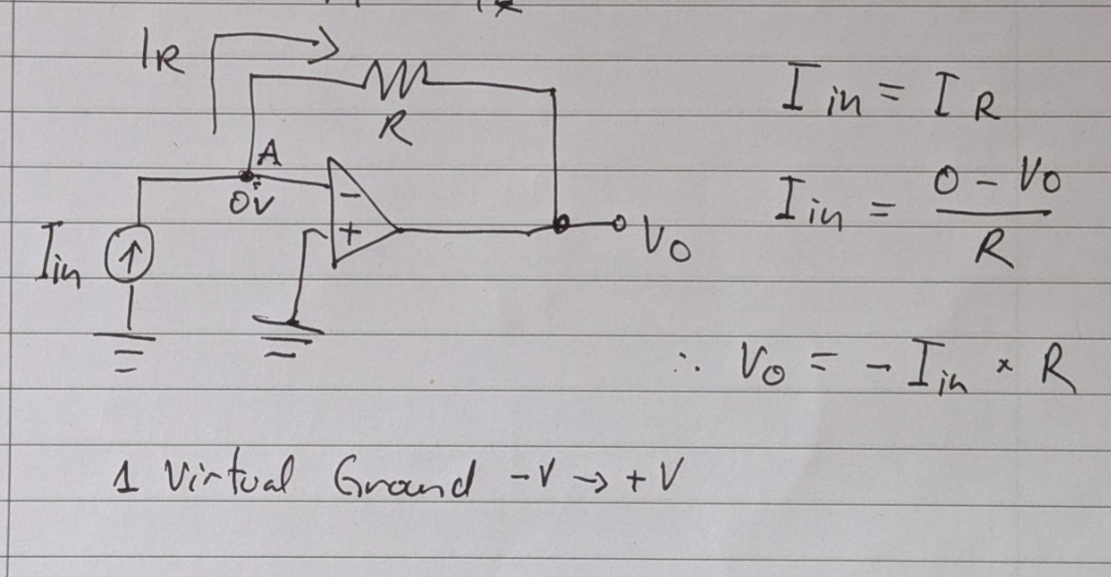
\includegraphics[width=0.8\textwidth]{figures/Appendix-DAQ/Vo_deriv.png}
    \caption{Solution Deriving TIA Vout}
    \label{fig:Vo_deriv}
  \end{figure}

\chapter{Appendix - Software Model Code}
\section{Section 1 Title}
\subsection{subsectiontitle}


\section{Section 2 Title}
\subsection{subsectiontitle}

%  appendix content in separate file^

\chapter{Further Appendix}
\section{Prototype Images}

\subsection{BreadBoard Prototype}
\begin{figure}[htbp]
    \centering
    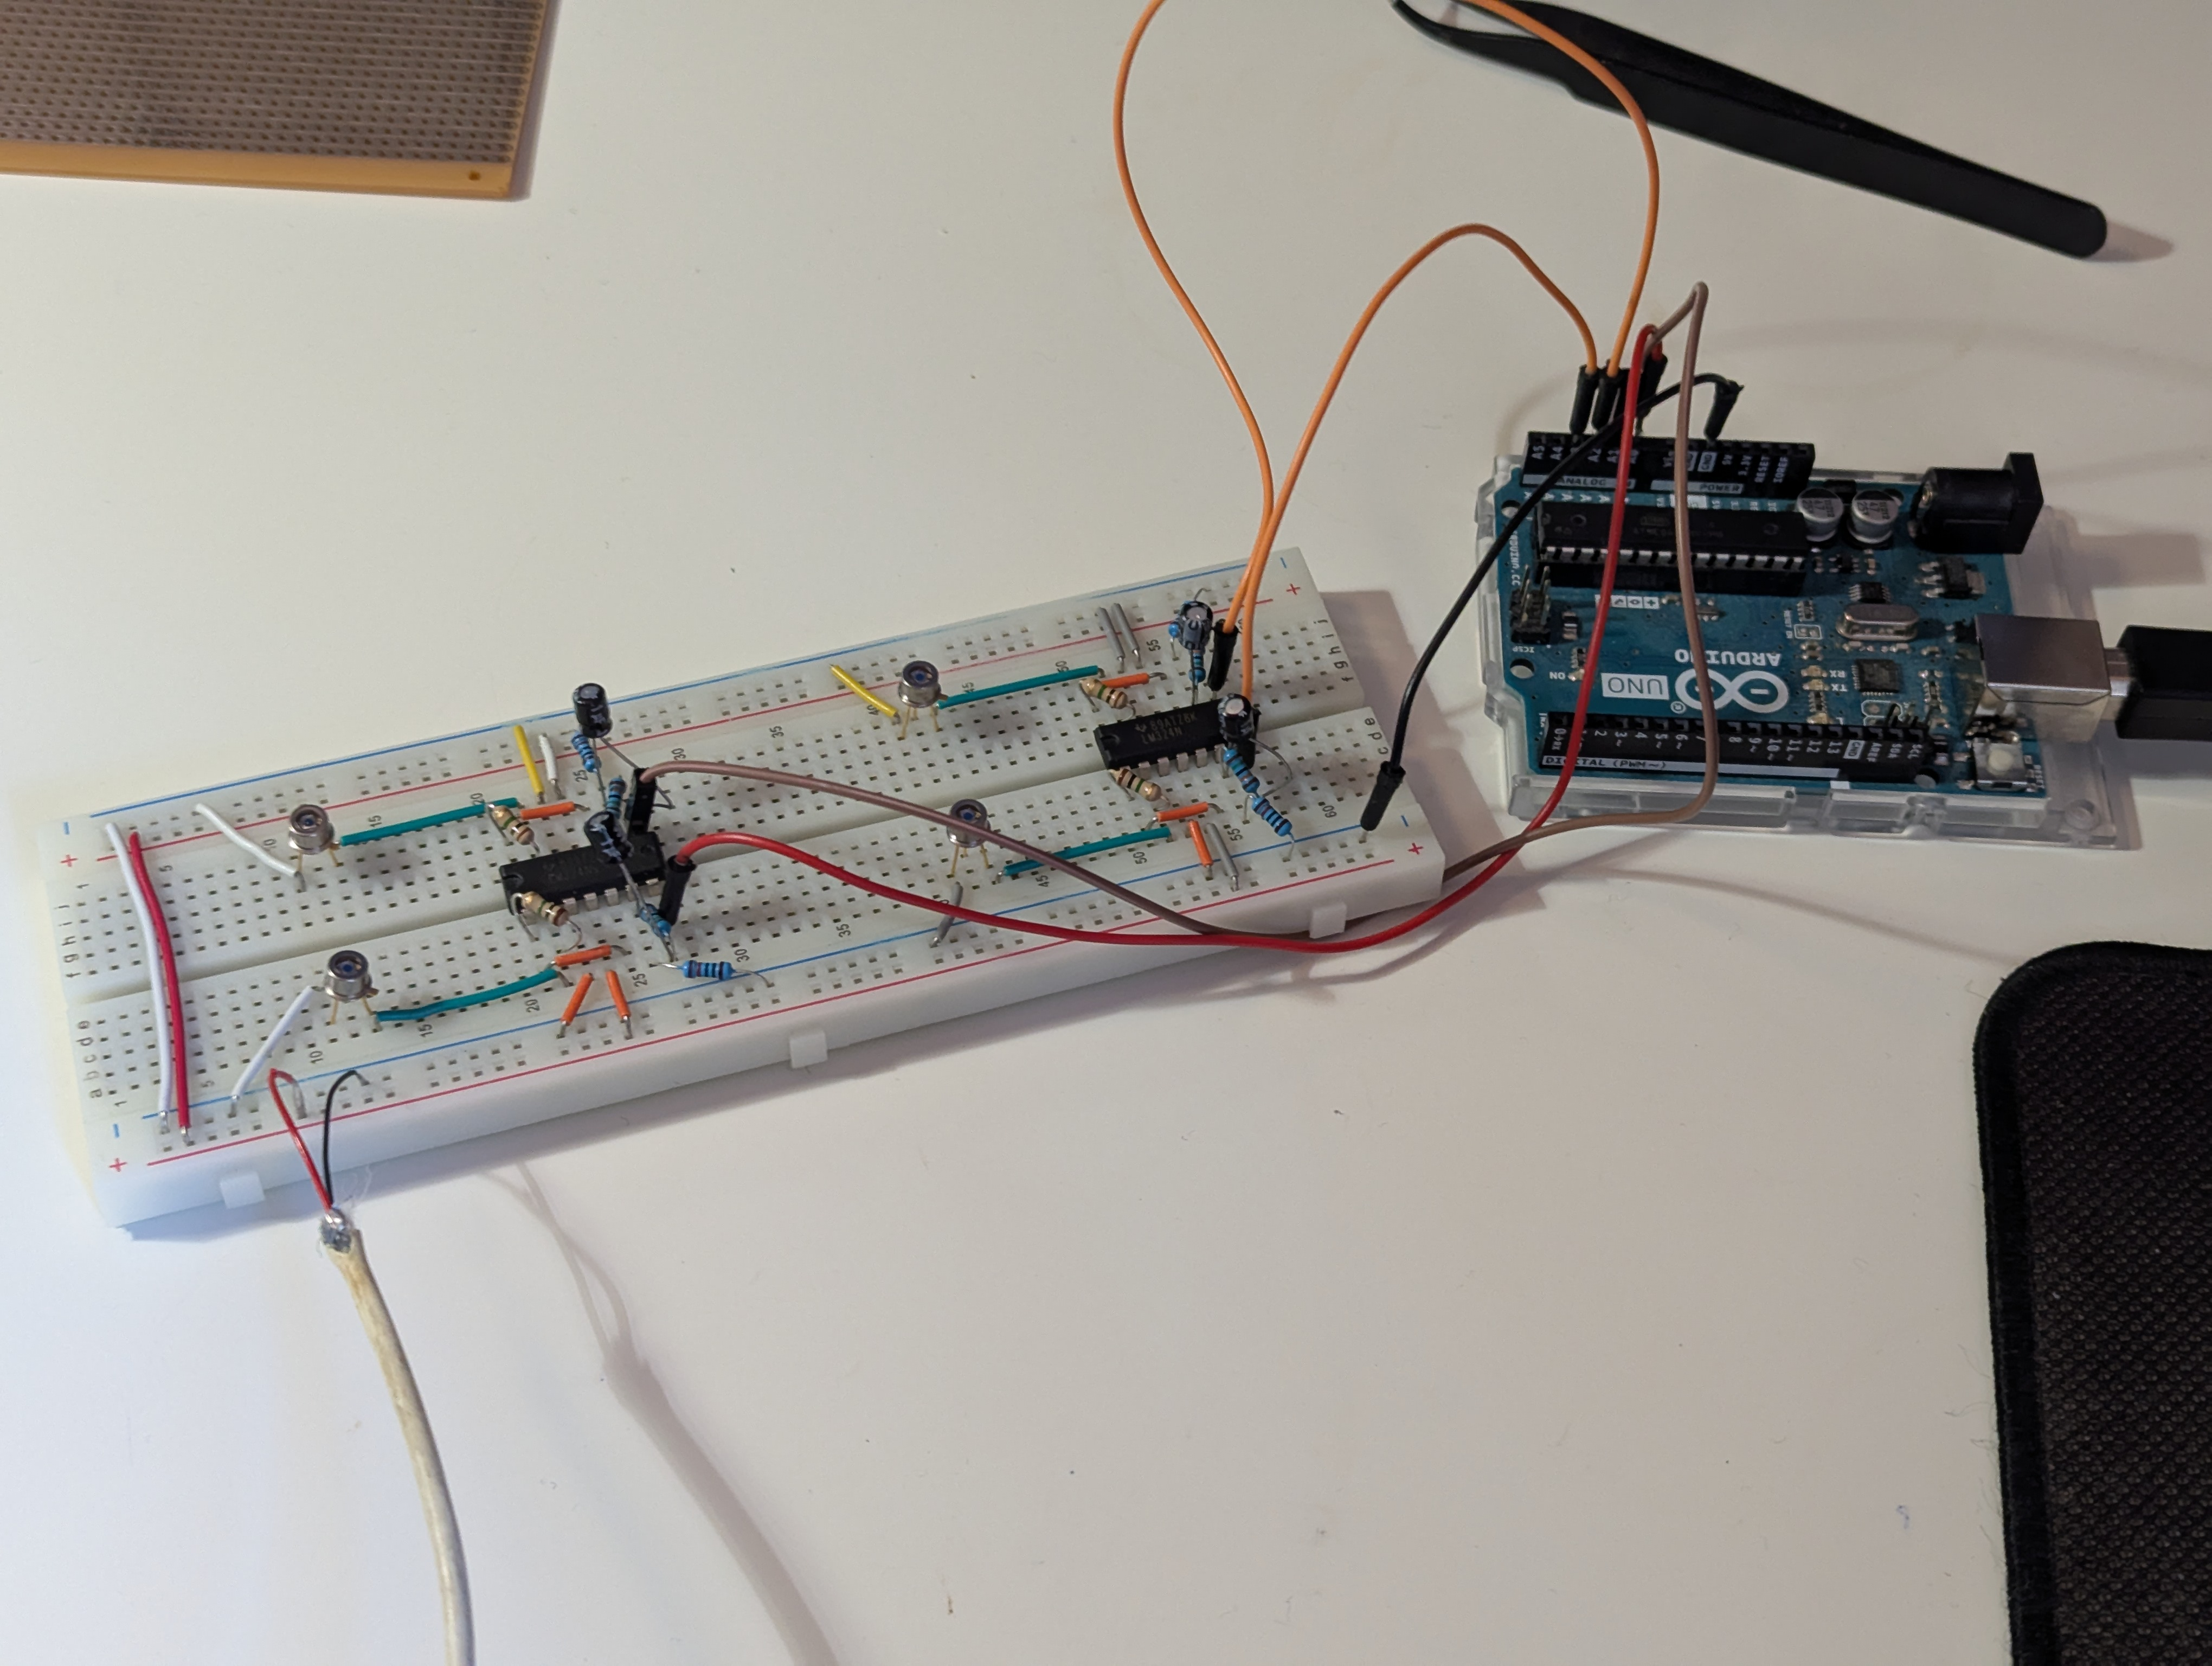
\includegraphics[width=0.7\textwidth]{figures/methodology/prototype_images/BreadBoard/BreadBoard_prototype.jpg}
    \caption*{Intial BreadBoard Prototype of the Photodiode Circuit} 
    \label{fig:BreadBoard-PrototypeLab}
    \end{figure}
\newpage
%%%%%%%%%%%%%%%%%%%%%%%%%%%%%%%%%%%%%%%%%%%%%%%%%%%%%%%%%%%
\subsection{Building the Prototype}
\begin{figure}[h]
    \centering
    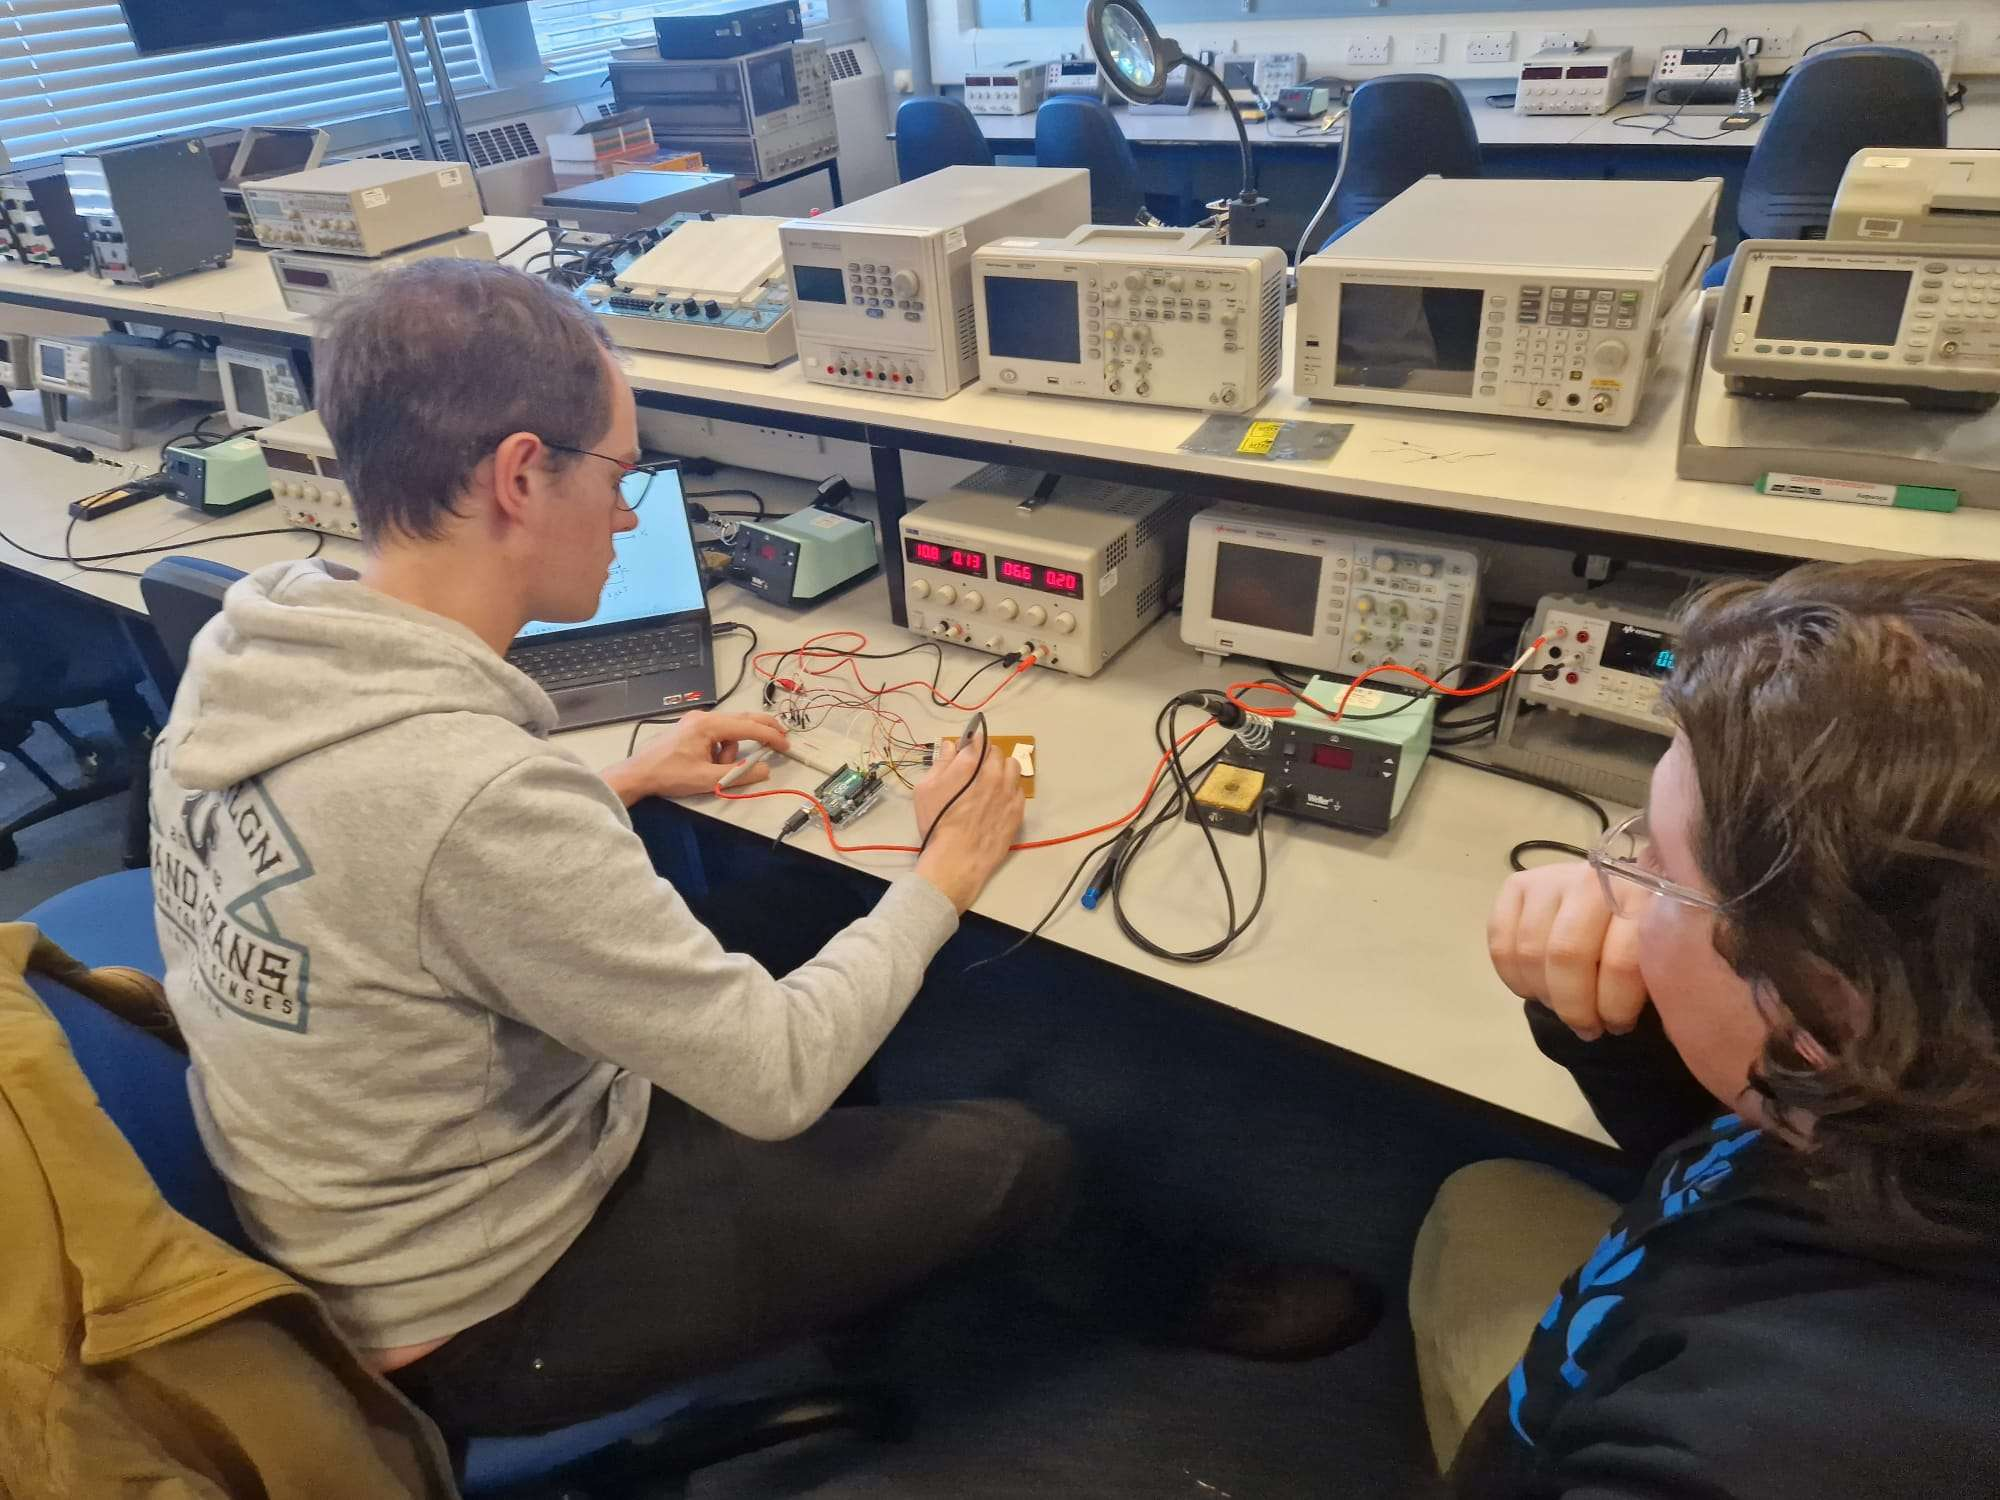
\includegraphics[width=0.7\textwidth]{figures/methodology/prototype_images/Building_The_Prototype/Lab_session1.jpg}
    \caption*{Lab Work for the Prototype (session 1)} 
    \label{fig:Lab-Session1}
    \end{figure}

\begin{figure}[htbp]
    \centering
    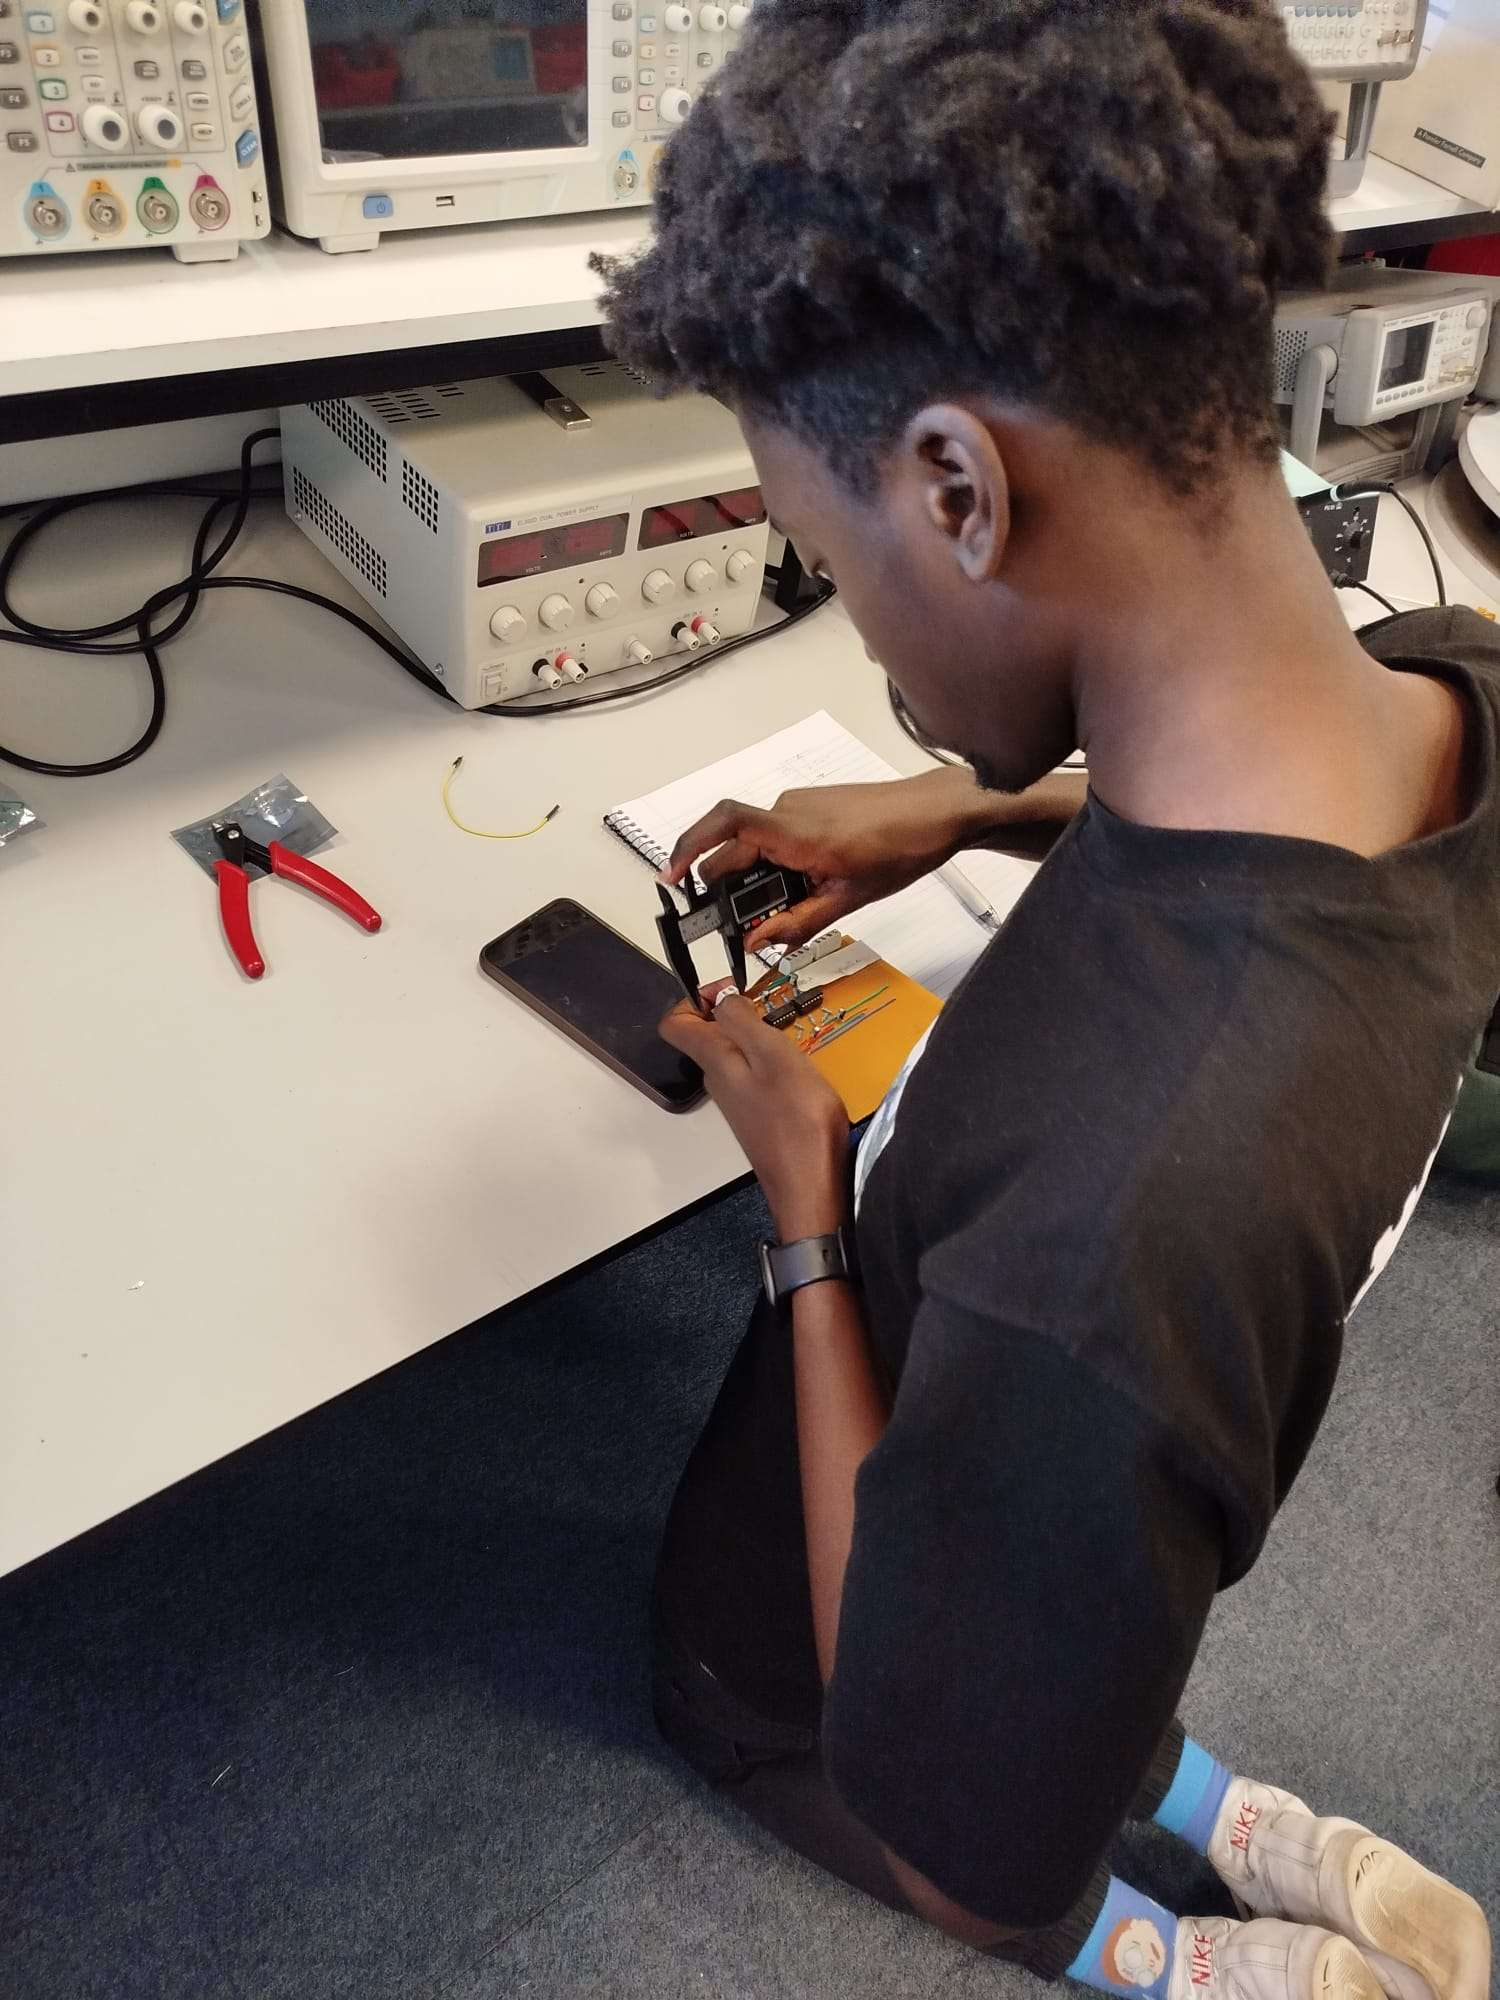
\includegraphics[width=0.7\textwidth]{figures/methodology/prototype_images/Building_The_Prototype/lab_session2.jpg}
    \caption*{lab Work for the Prototype (session 2)} 
    \label{fig:Lab-Session2}
\end{figure}
\newpage
%%%%%%%%%%%%%%%%%%%%%%%%%%%%%%%%%%%%%%%%%%%%%%%%%%%%%%%%%%%%
\subsection{Prototype Testing}
\begin{figure}[h]
    \centering
    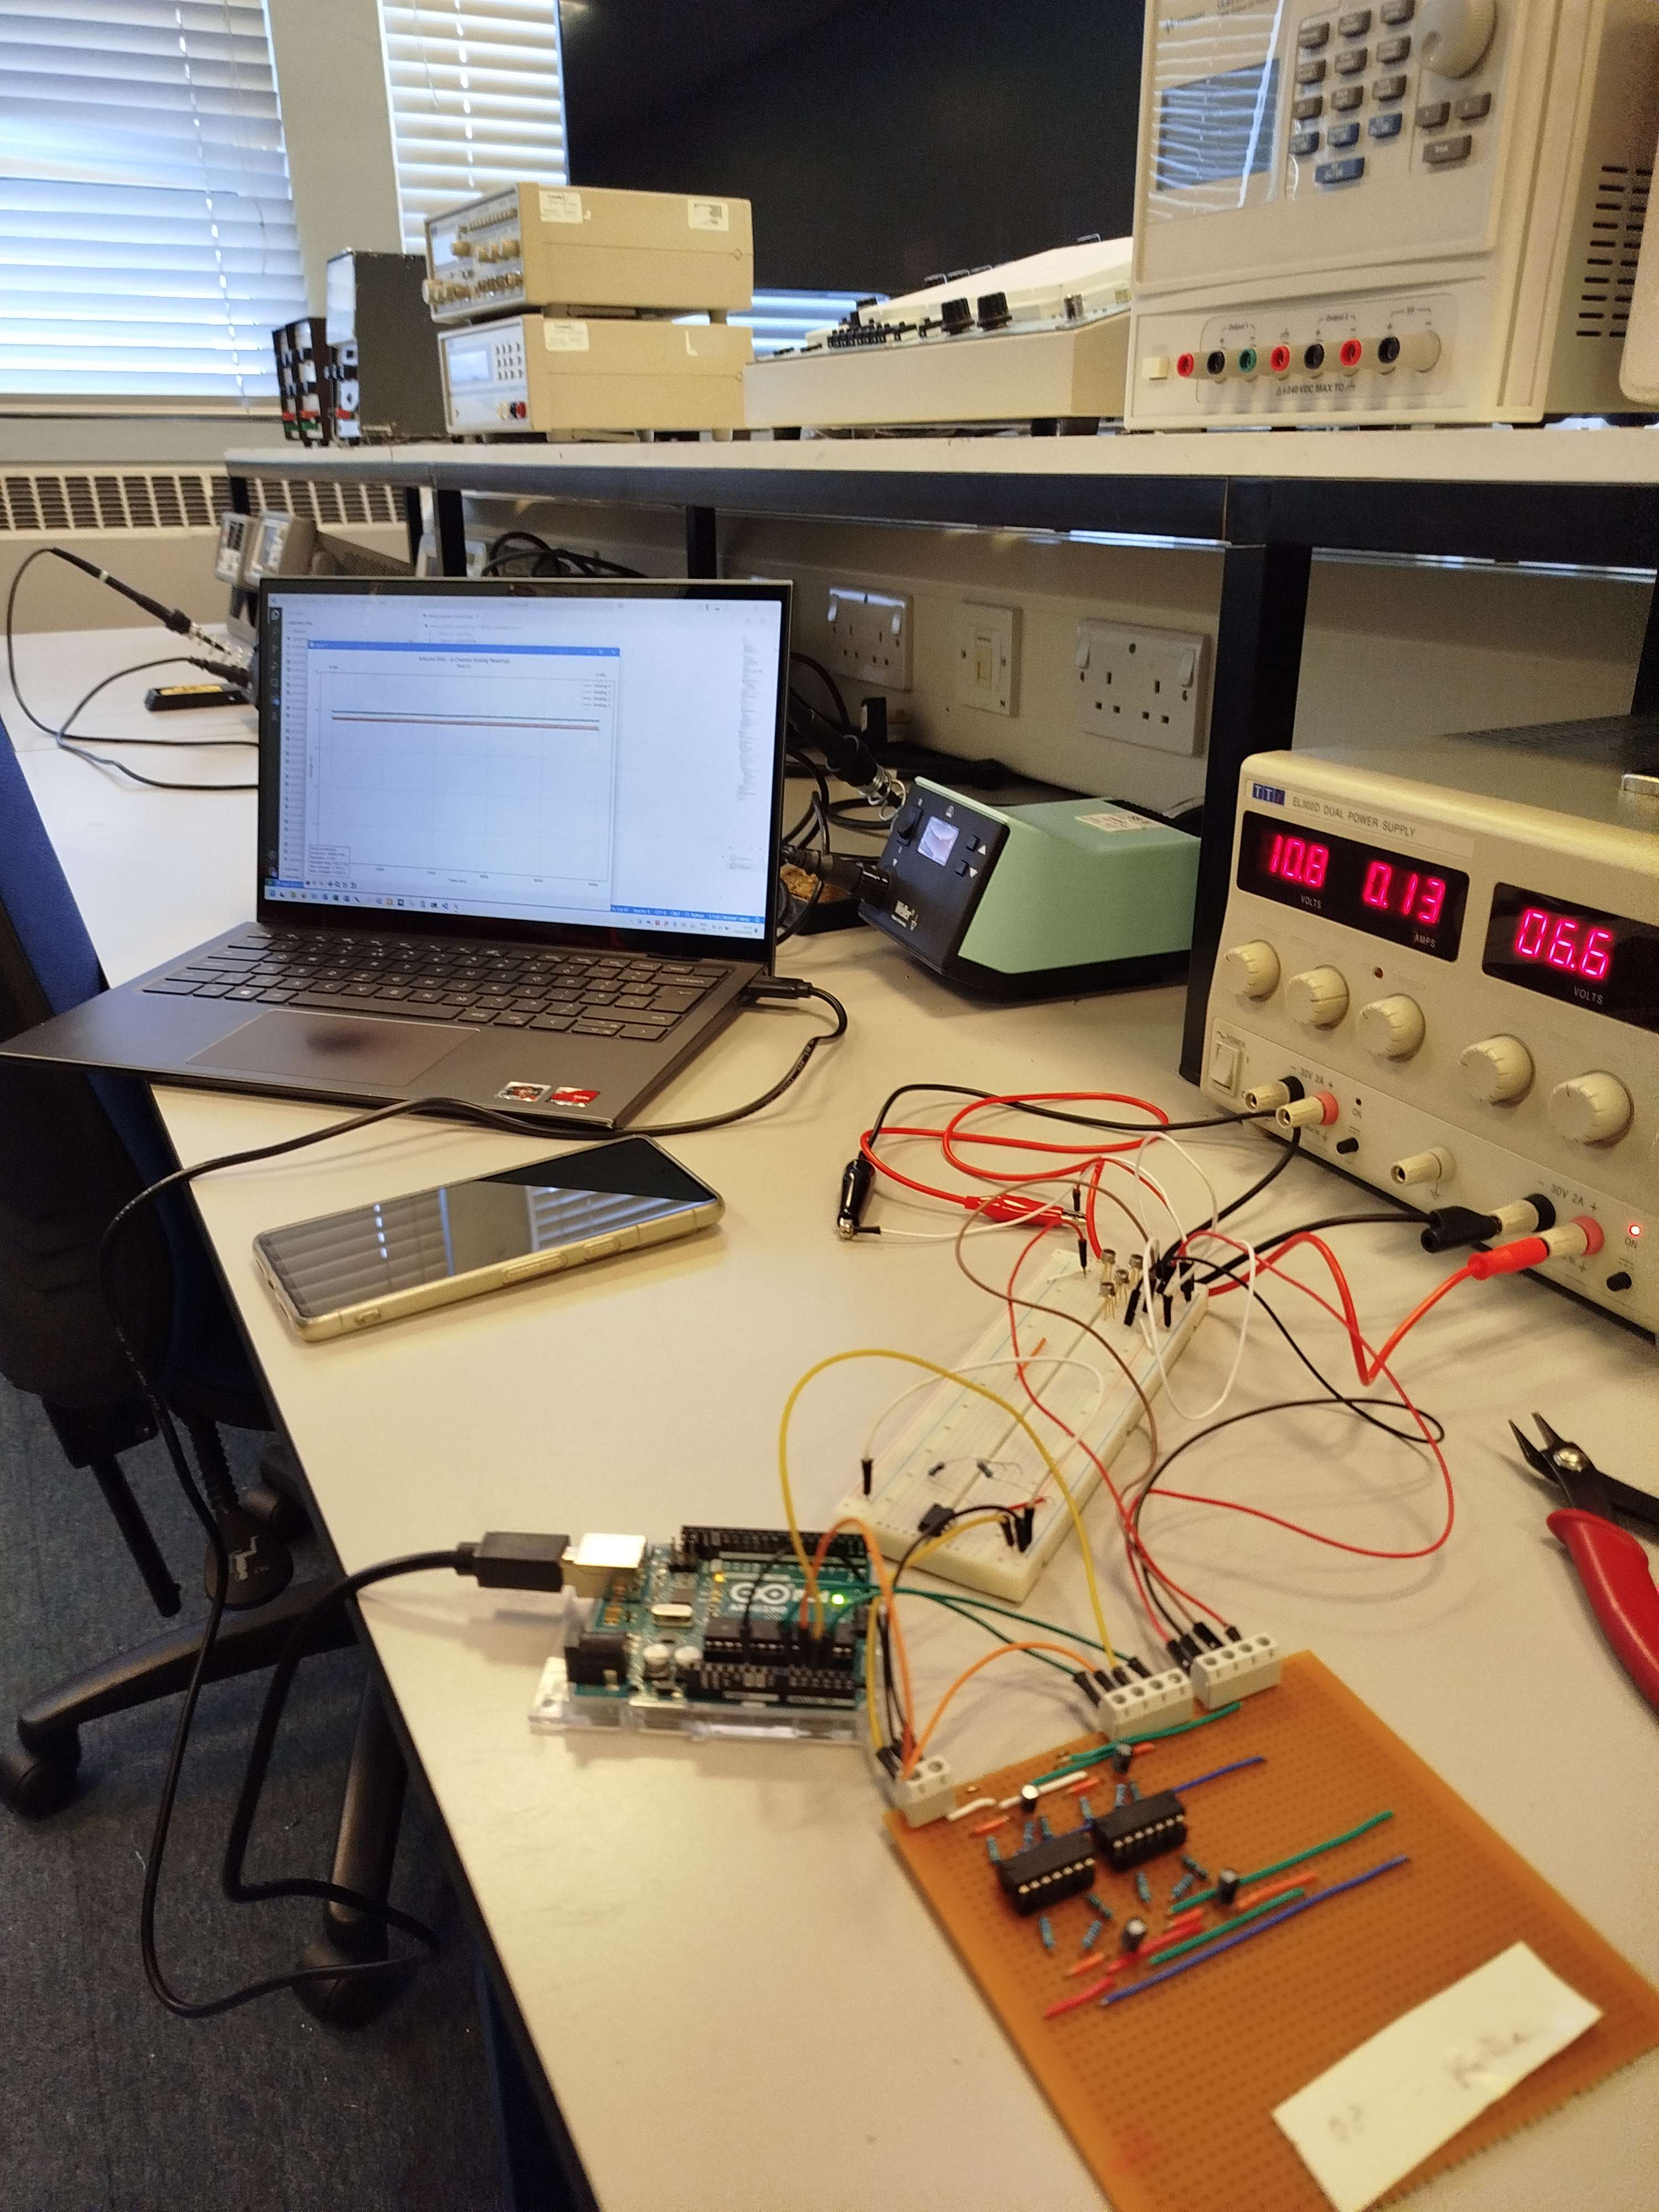
\includegraphics[width=0.7\textwidth]{figures/methodology/Prototype_testing/first_lab_test_of_prototype.jpg}
    \caption*{First Lab Test of the Prototype} 
    \label{fig:First-Lab-Testing-Prototype}
\end{figure}
\newpage
%%%%%%%%%%%%%%%%%%%%%%%%%%%%%%%%%%%%%%%%%%%%%%%%%%%%%%%%%%%%%%%%
\subsection{RED testbench}
\begin{figure}[h]
    \centering
    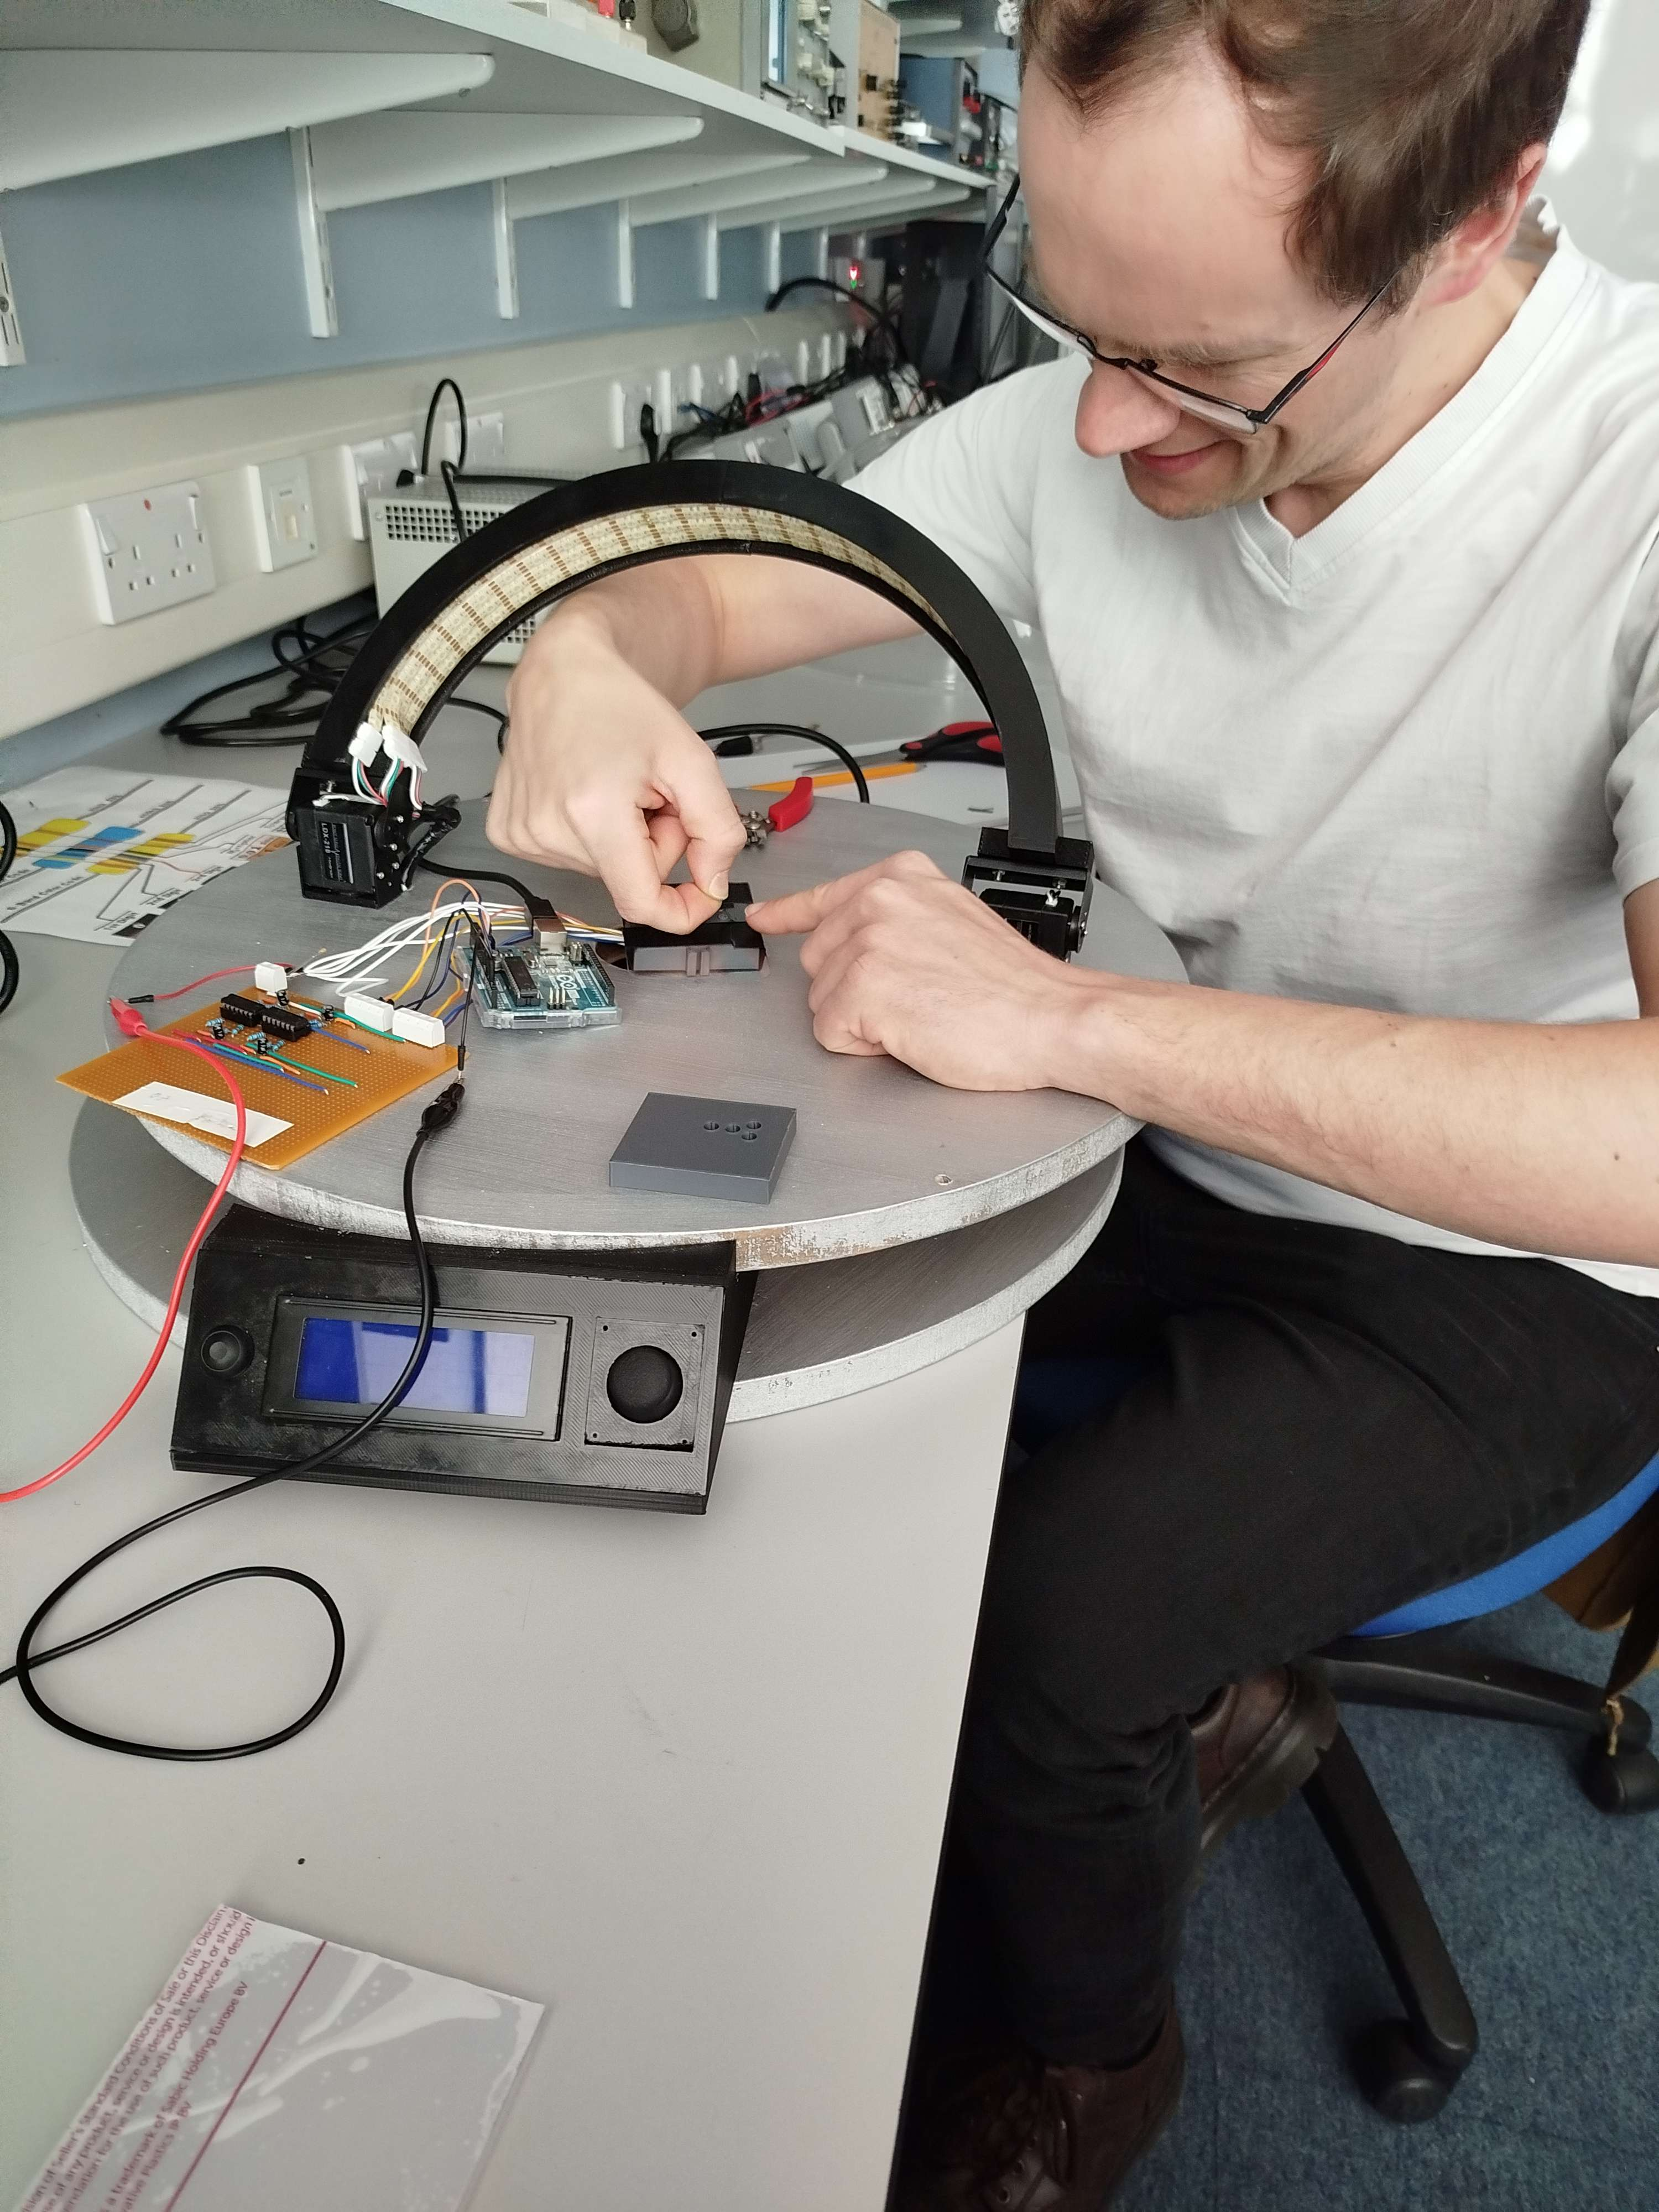
\includegraphics[width=0.7\textwidth]{figures/methodology/The_Arch/building_the_setup.jpg}
    \caption*{RED Testbench 1} 
    \label{fig:RED-Testbench1}
\end{figure}
\newpage
 %%%%%%%%%%%%%%%%%%%%%%%%%%%%%%%%%%%%%   
\subsection{Solar Lab Prototype Testing}

\begin{figure}[htbp]
    \centering
    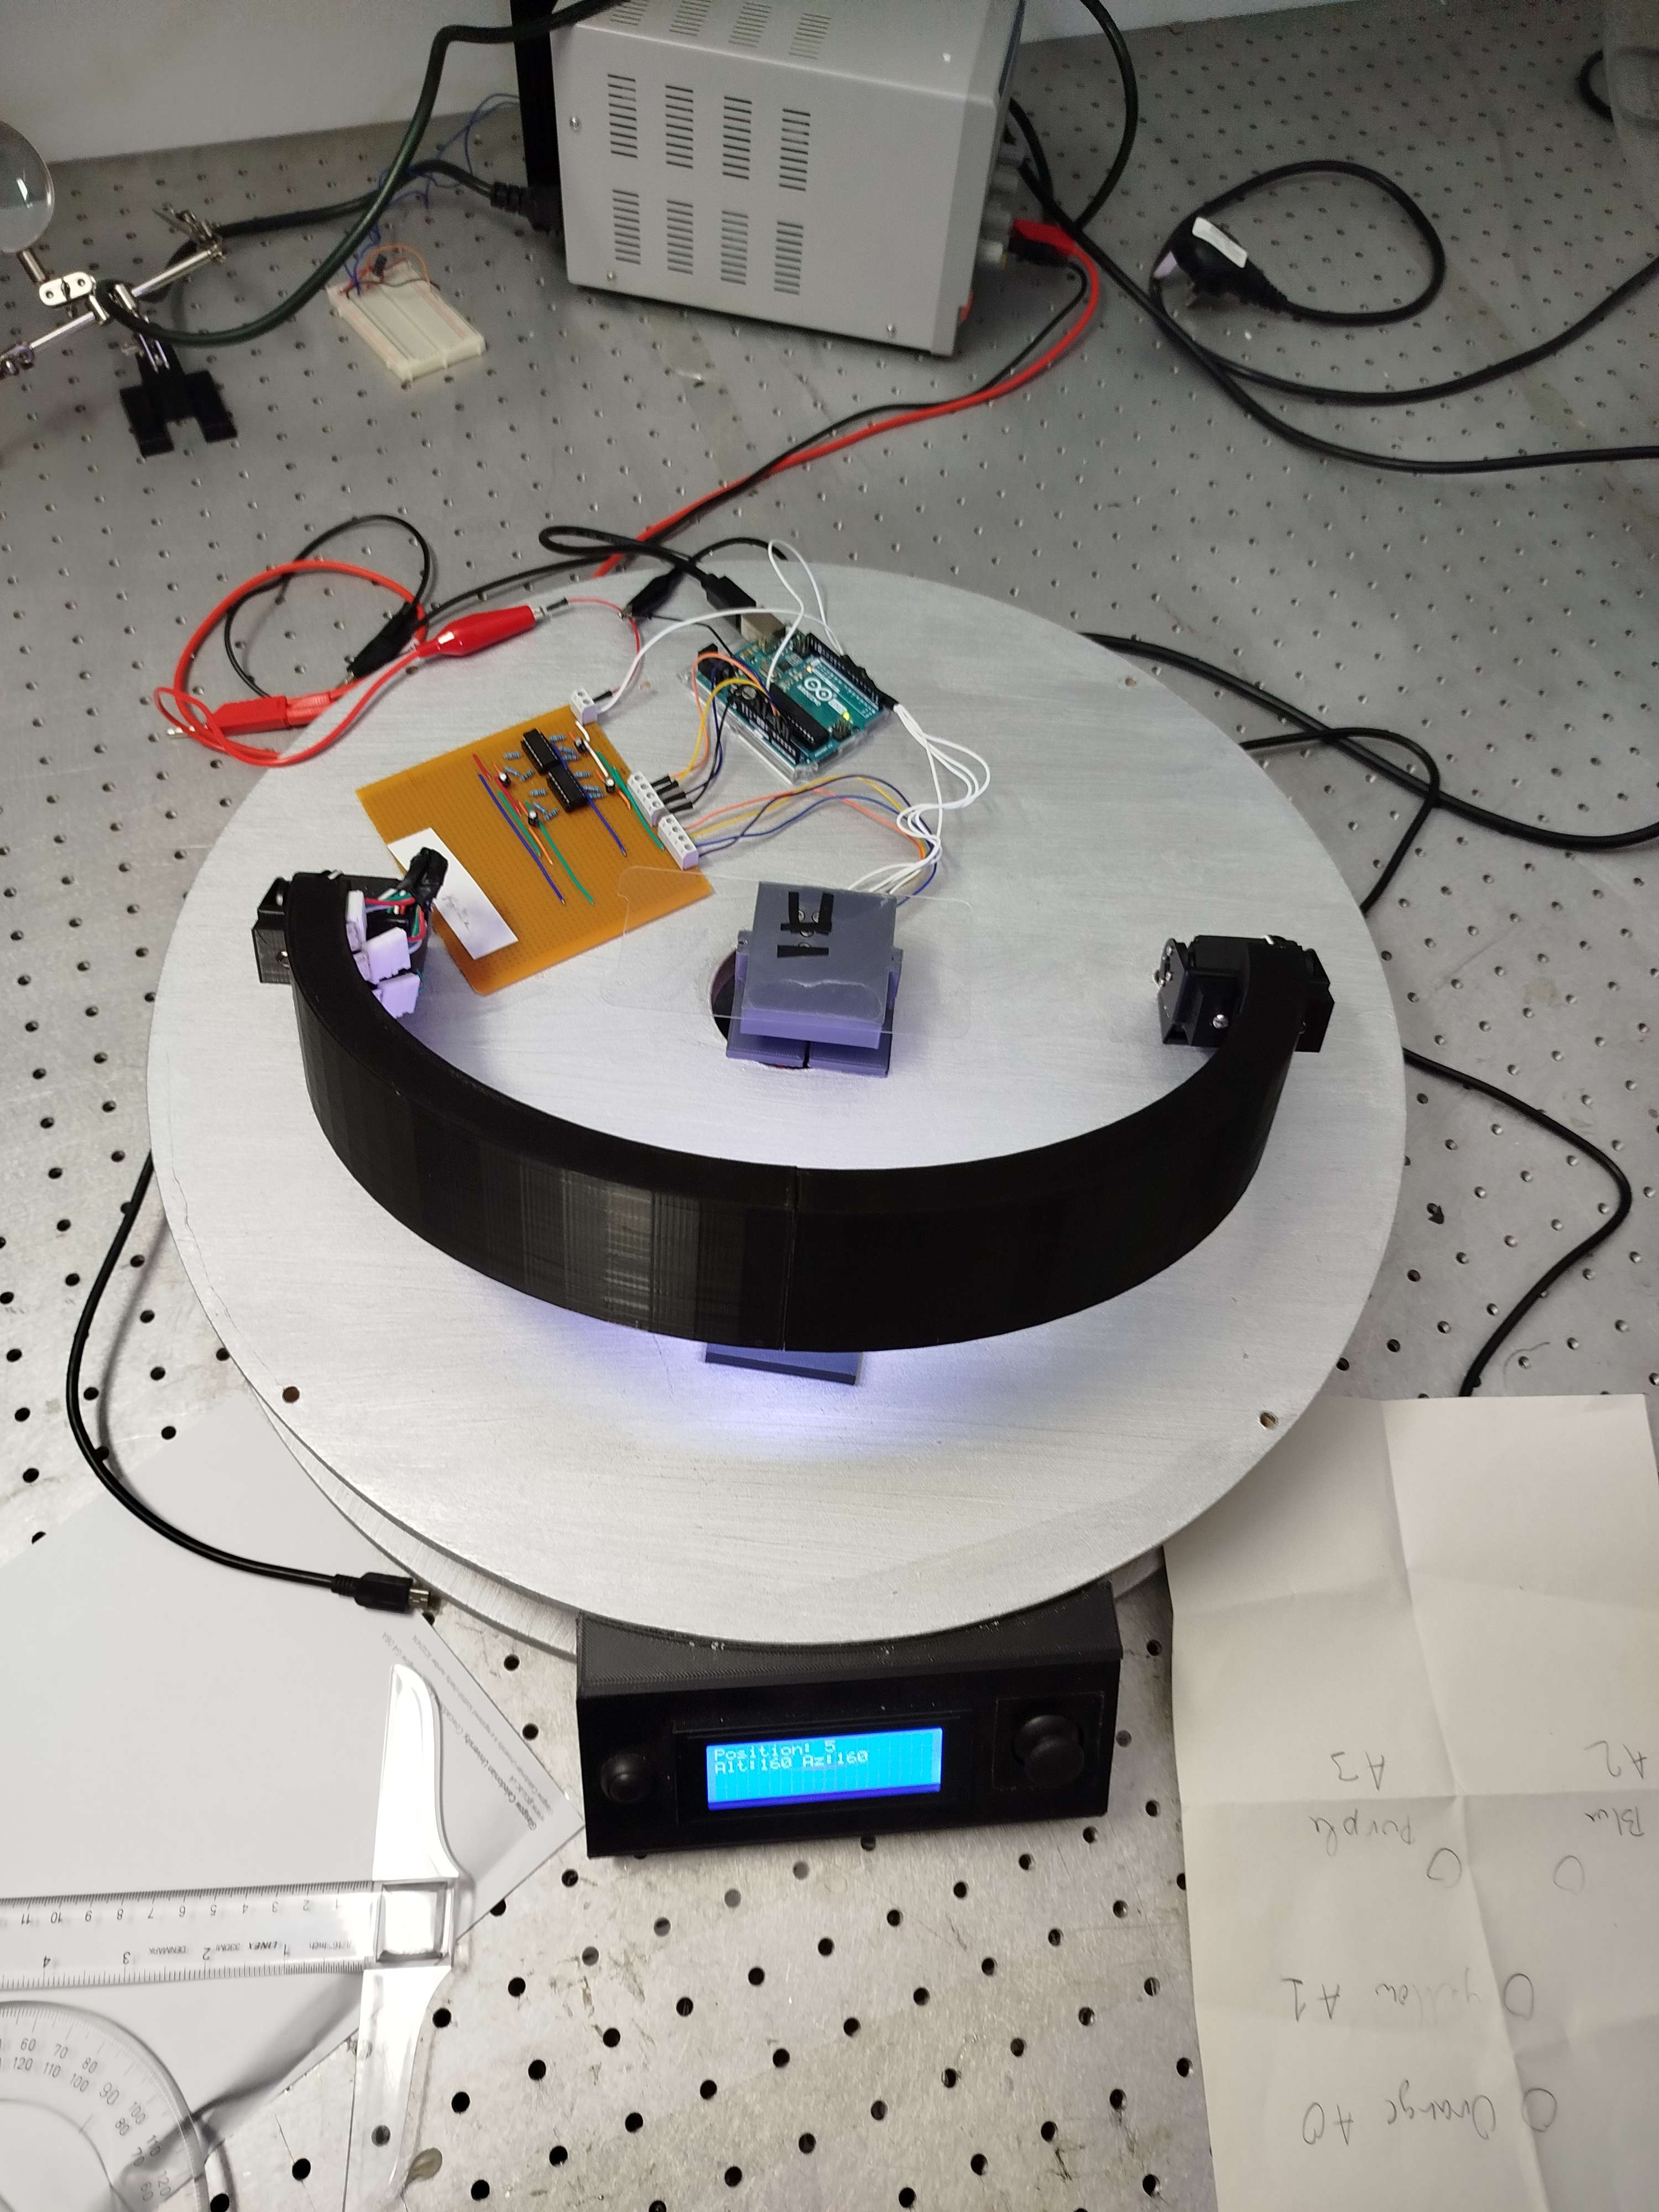
\includegraphics[width=0.7\textwidth]{figures/methodology/Prototype_testing/solarLab_test1.jpg}
    \caption*{Solar Lab Test of the Prototype 1} 
    \label{fig:Solar-Lab-Test-Prototype1}
    \end{figure}

\begin{figure}[htbp]
    \centering
    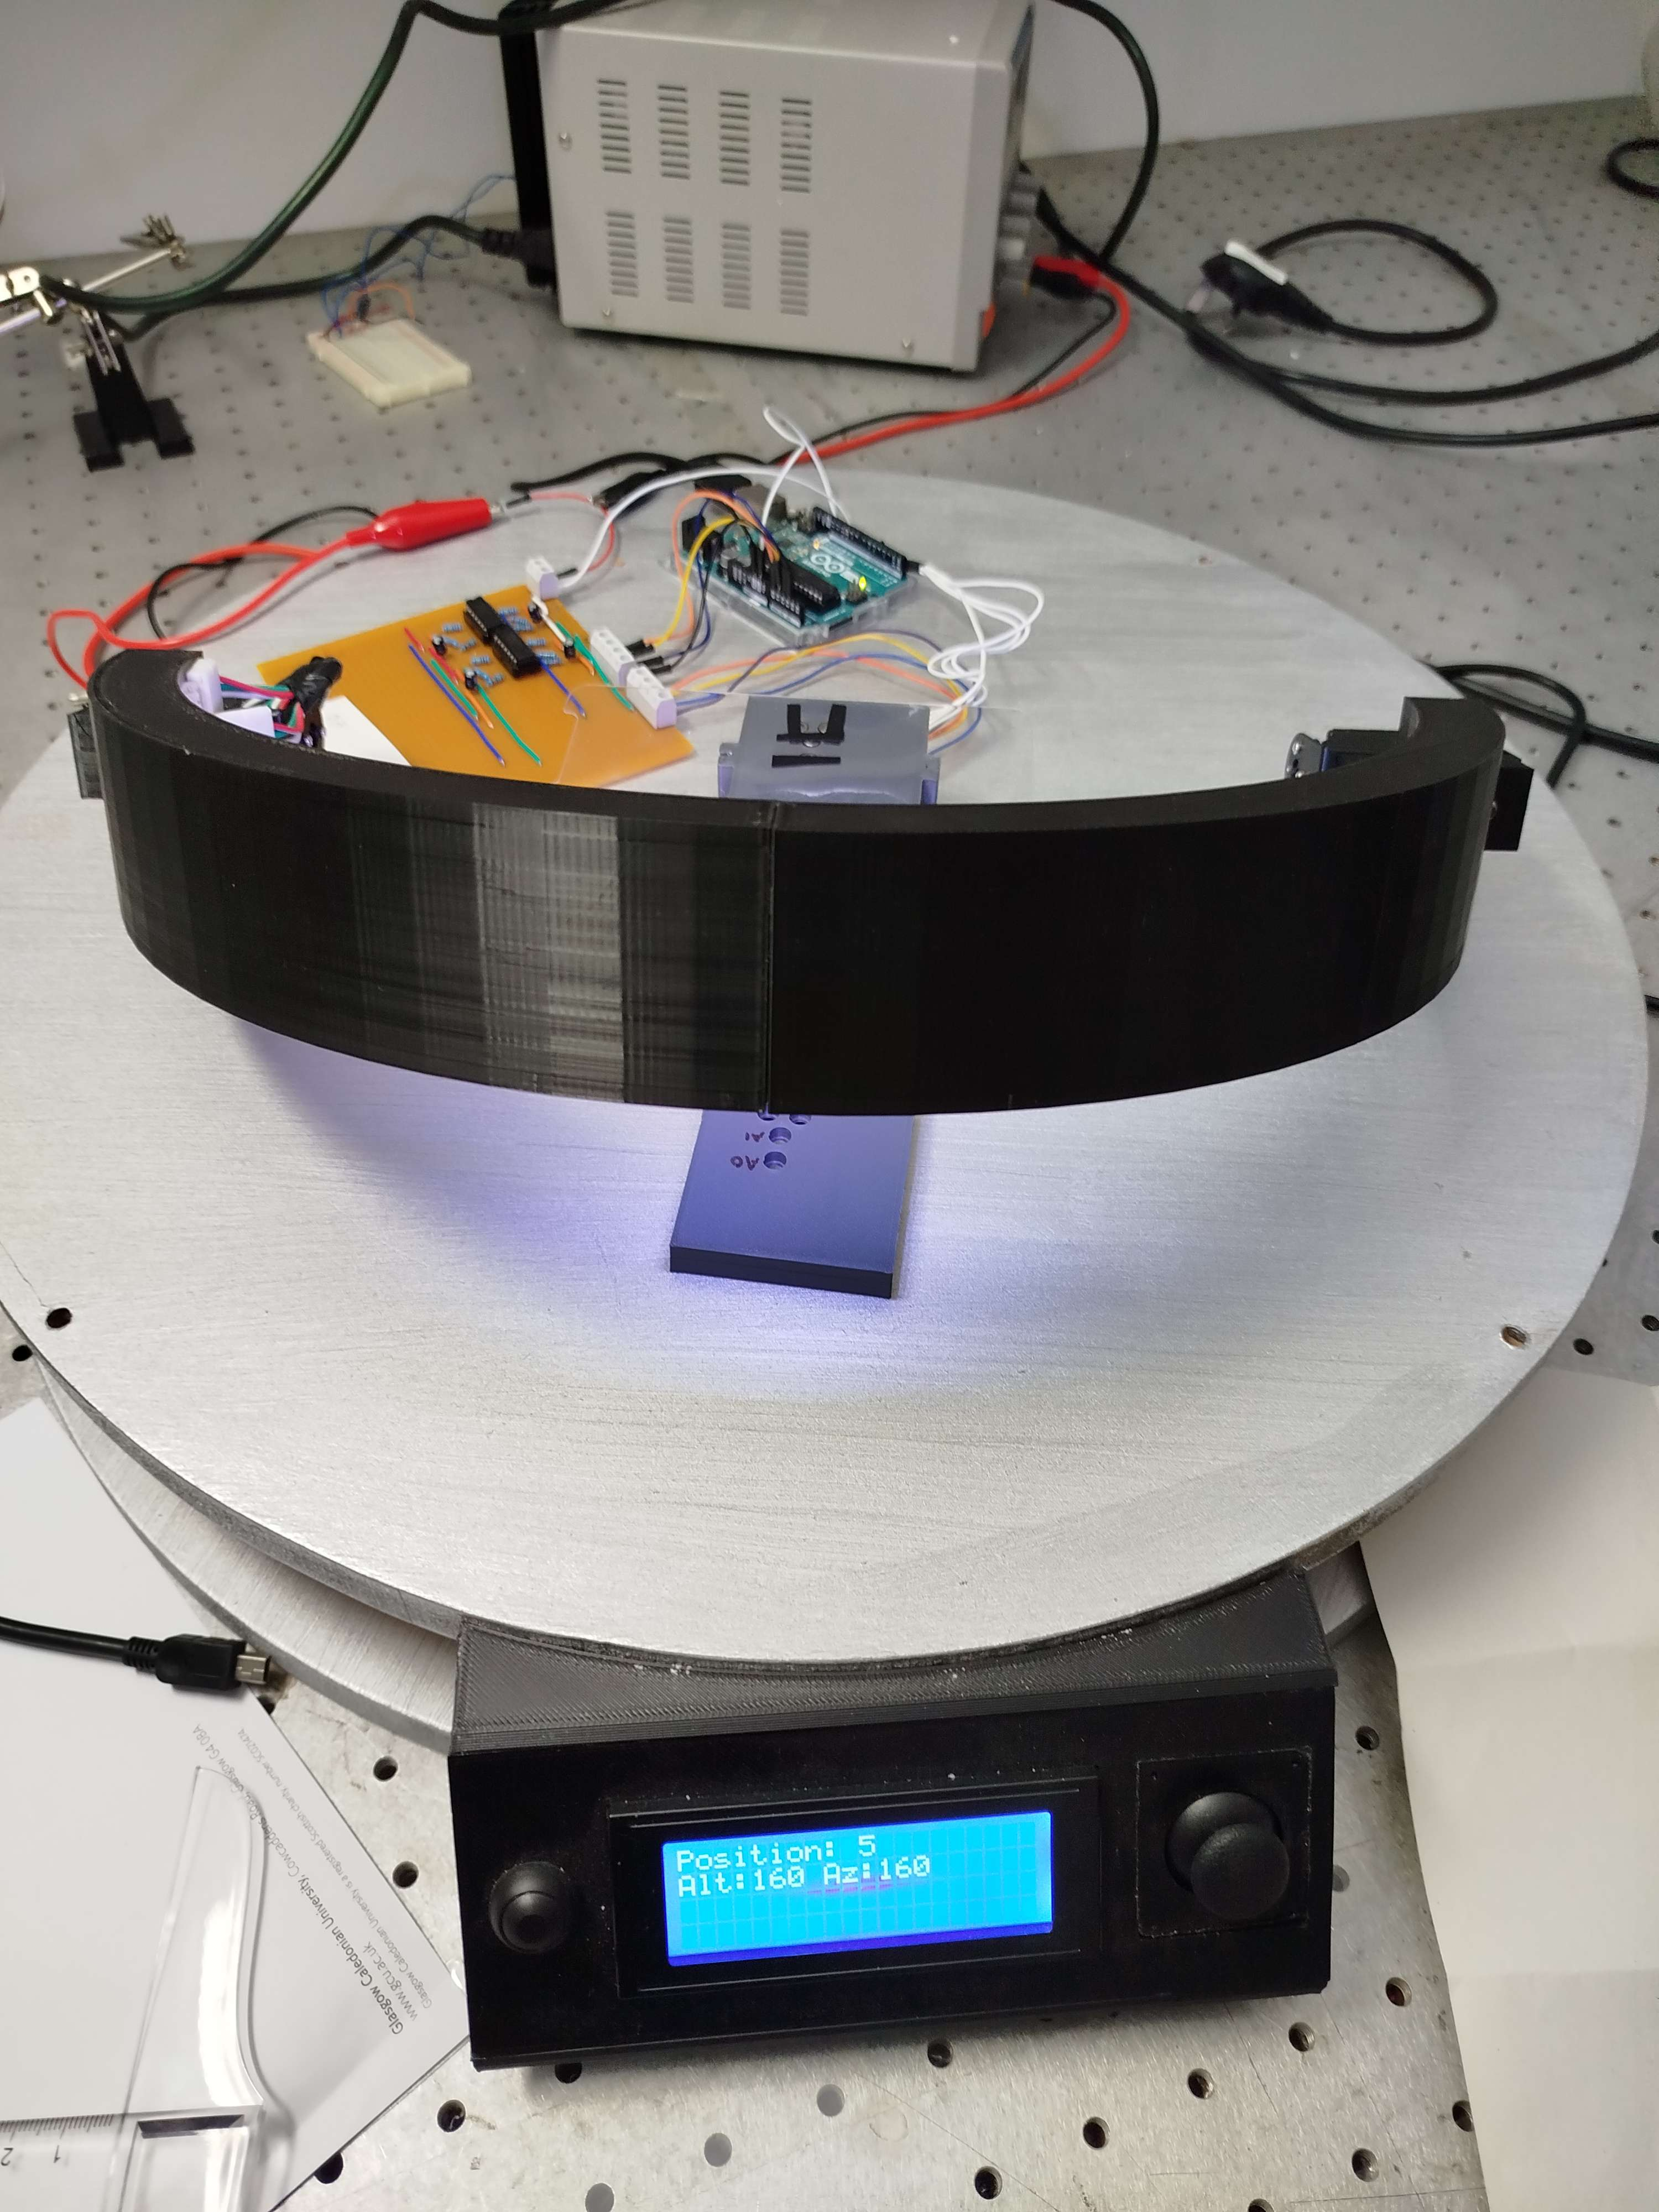
\includegraphics[width=0.7\textwidth]{figures/methodology/Prototype_testing/solarLab_test2.jpg}
    \caption*{Solar Lab Test of the Prototype 2} 
    \label{fig:Solar-Lab-Test-Prototype2}
\end{figure}

\begin{figure}[htbp]
    \centering
    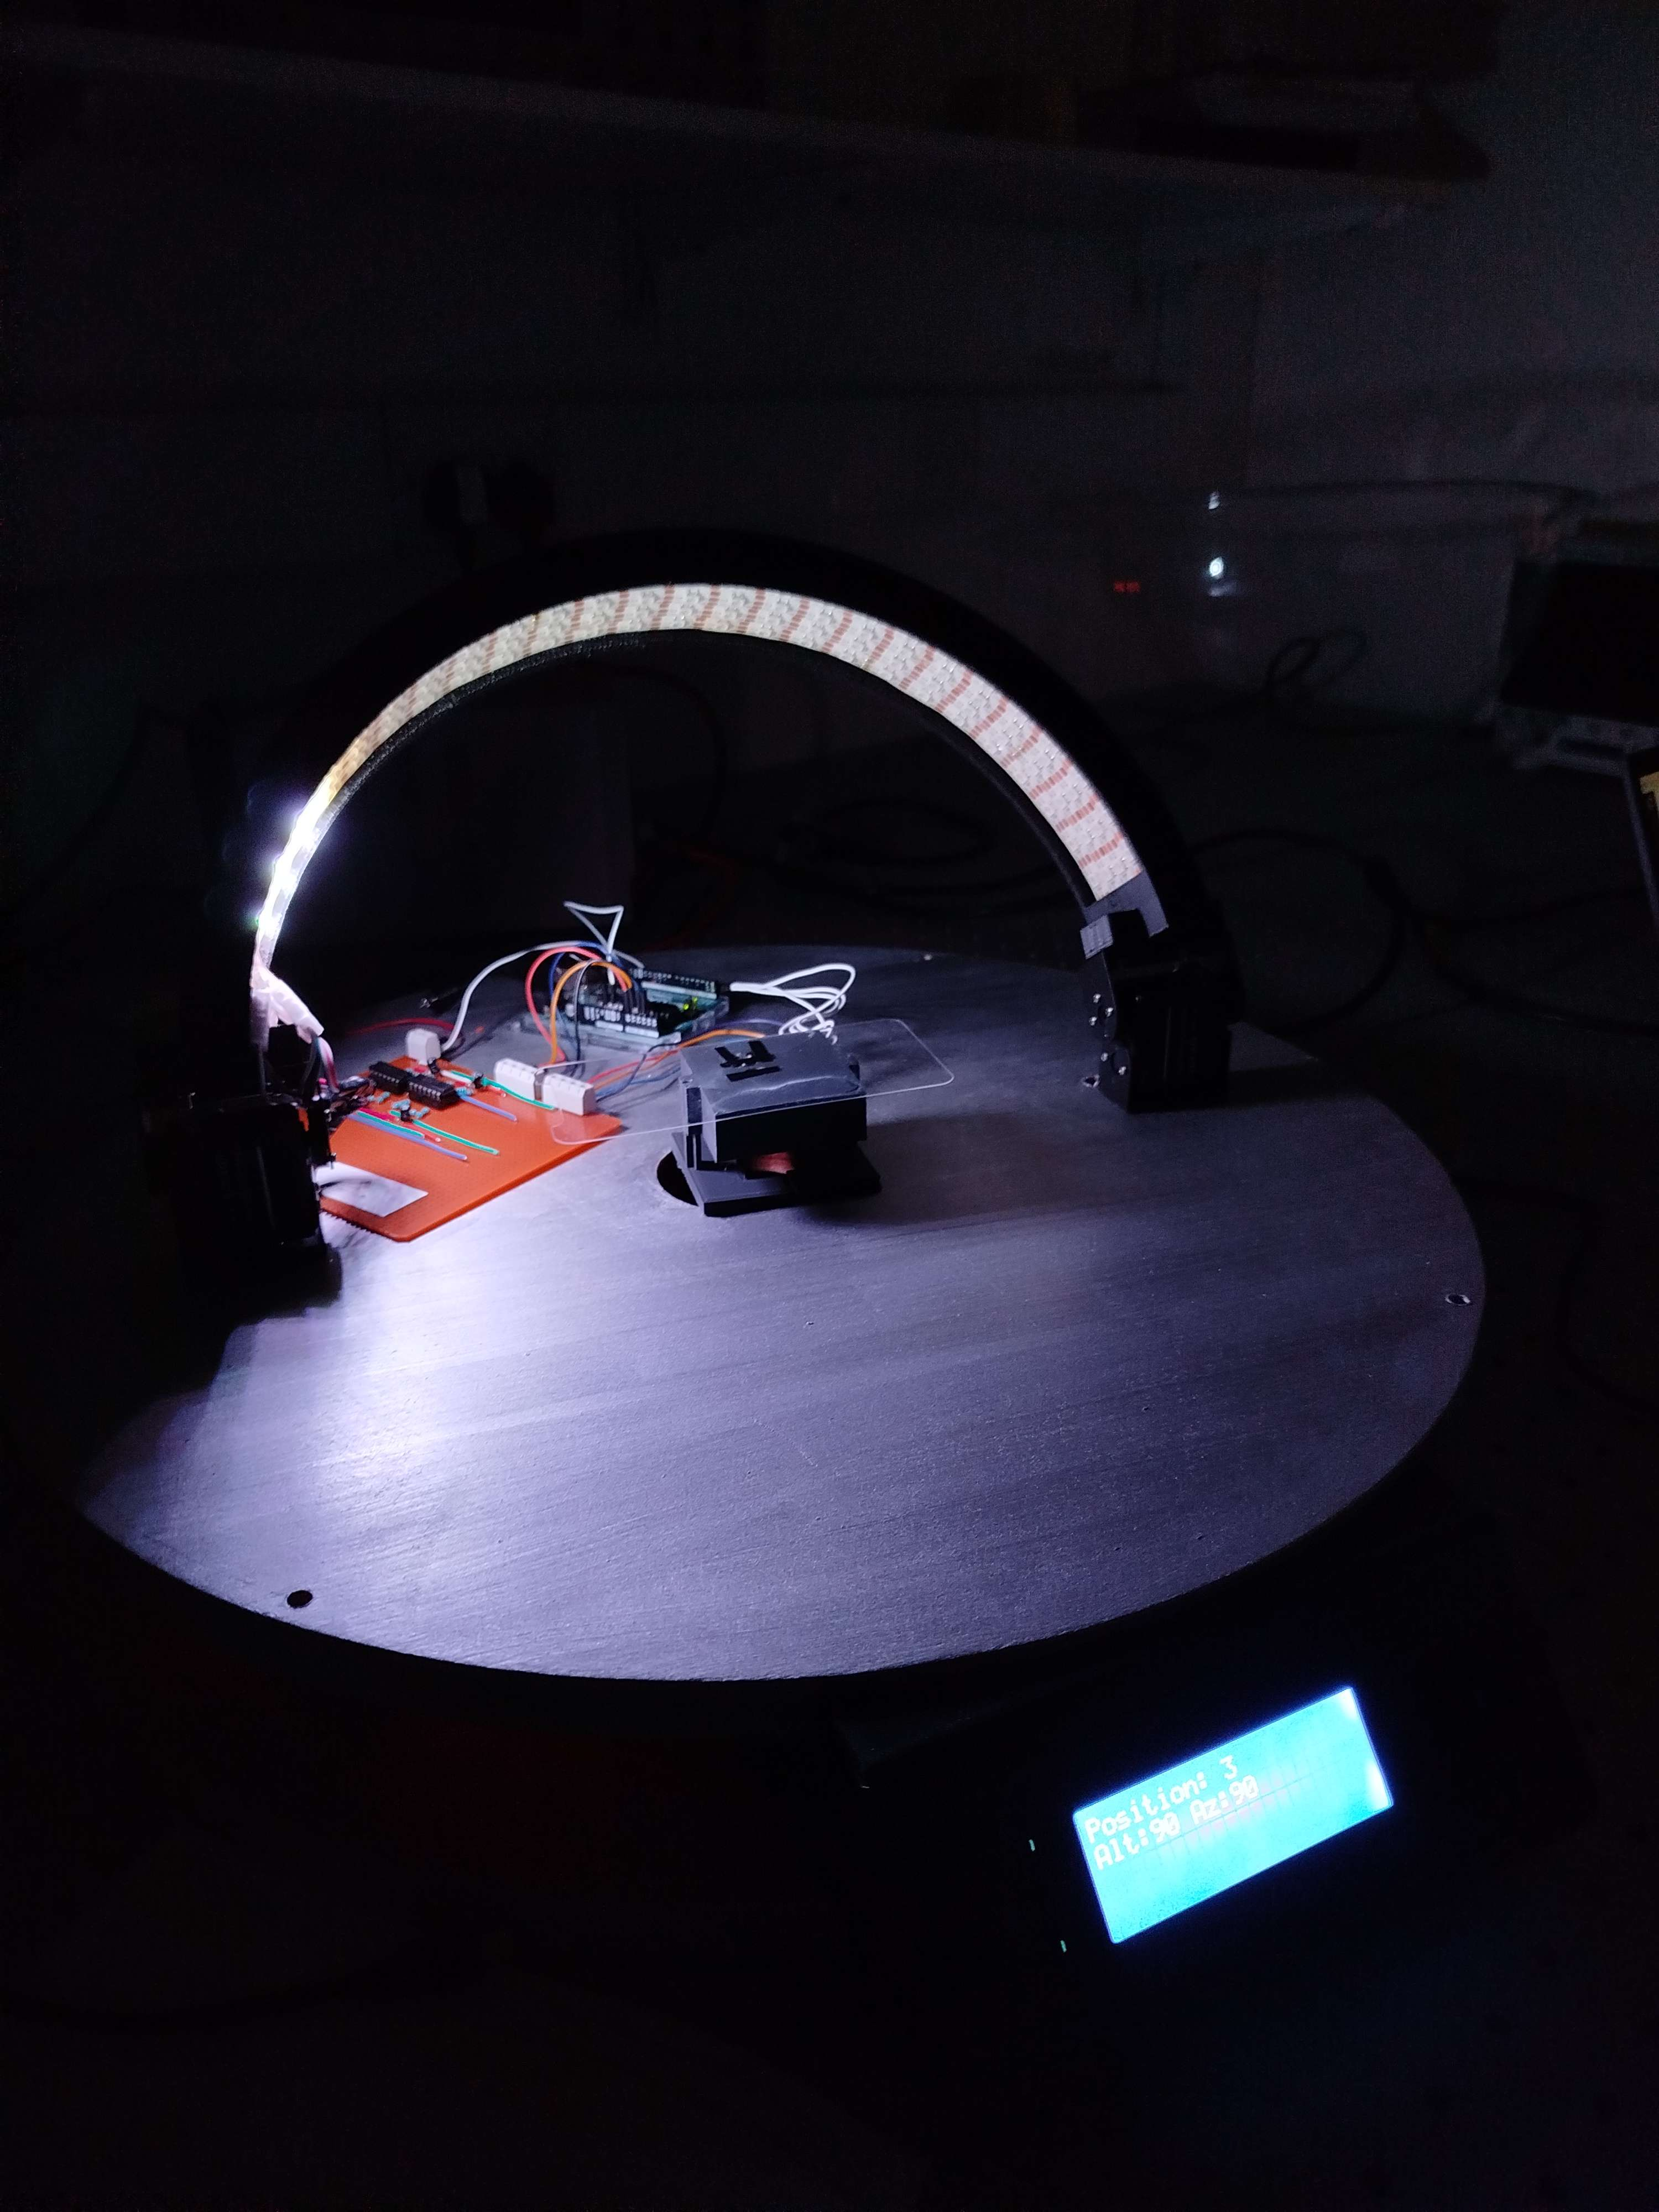
\includegraphics[width=0.7\textwidth]{figures/methodology/Prototype_testing/solarLab_test3.jpg}
    \caption*{Solar Lab Test of the Prototype 3} 
    \label{fig:Solar-Lab-Test-Prototype3}
\end{figure}

\begin{figure}[htbp]
     \centering
     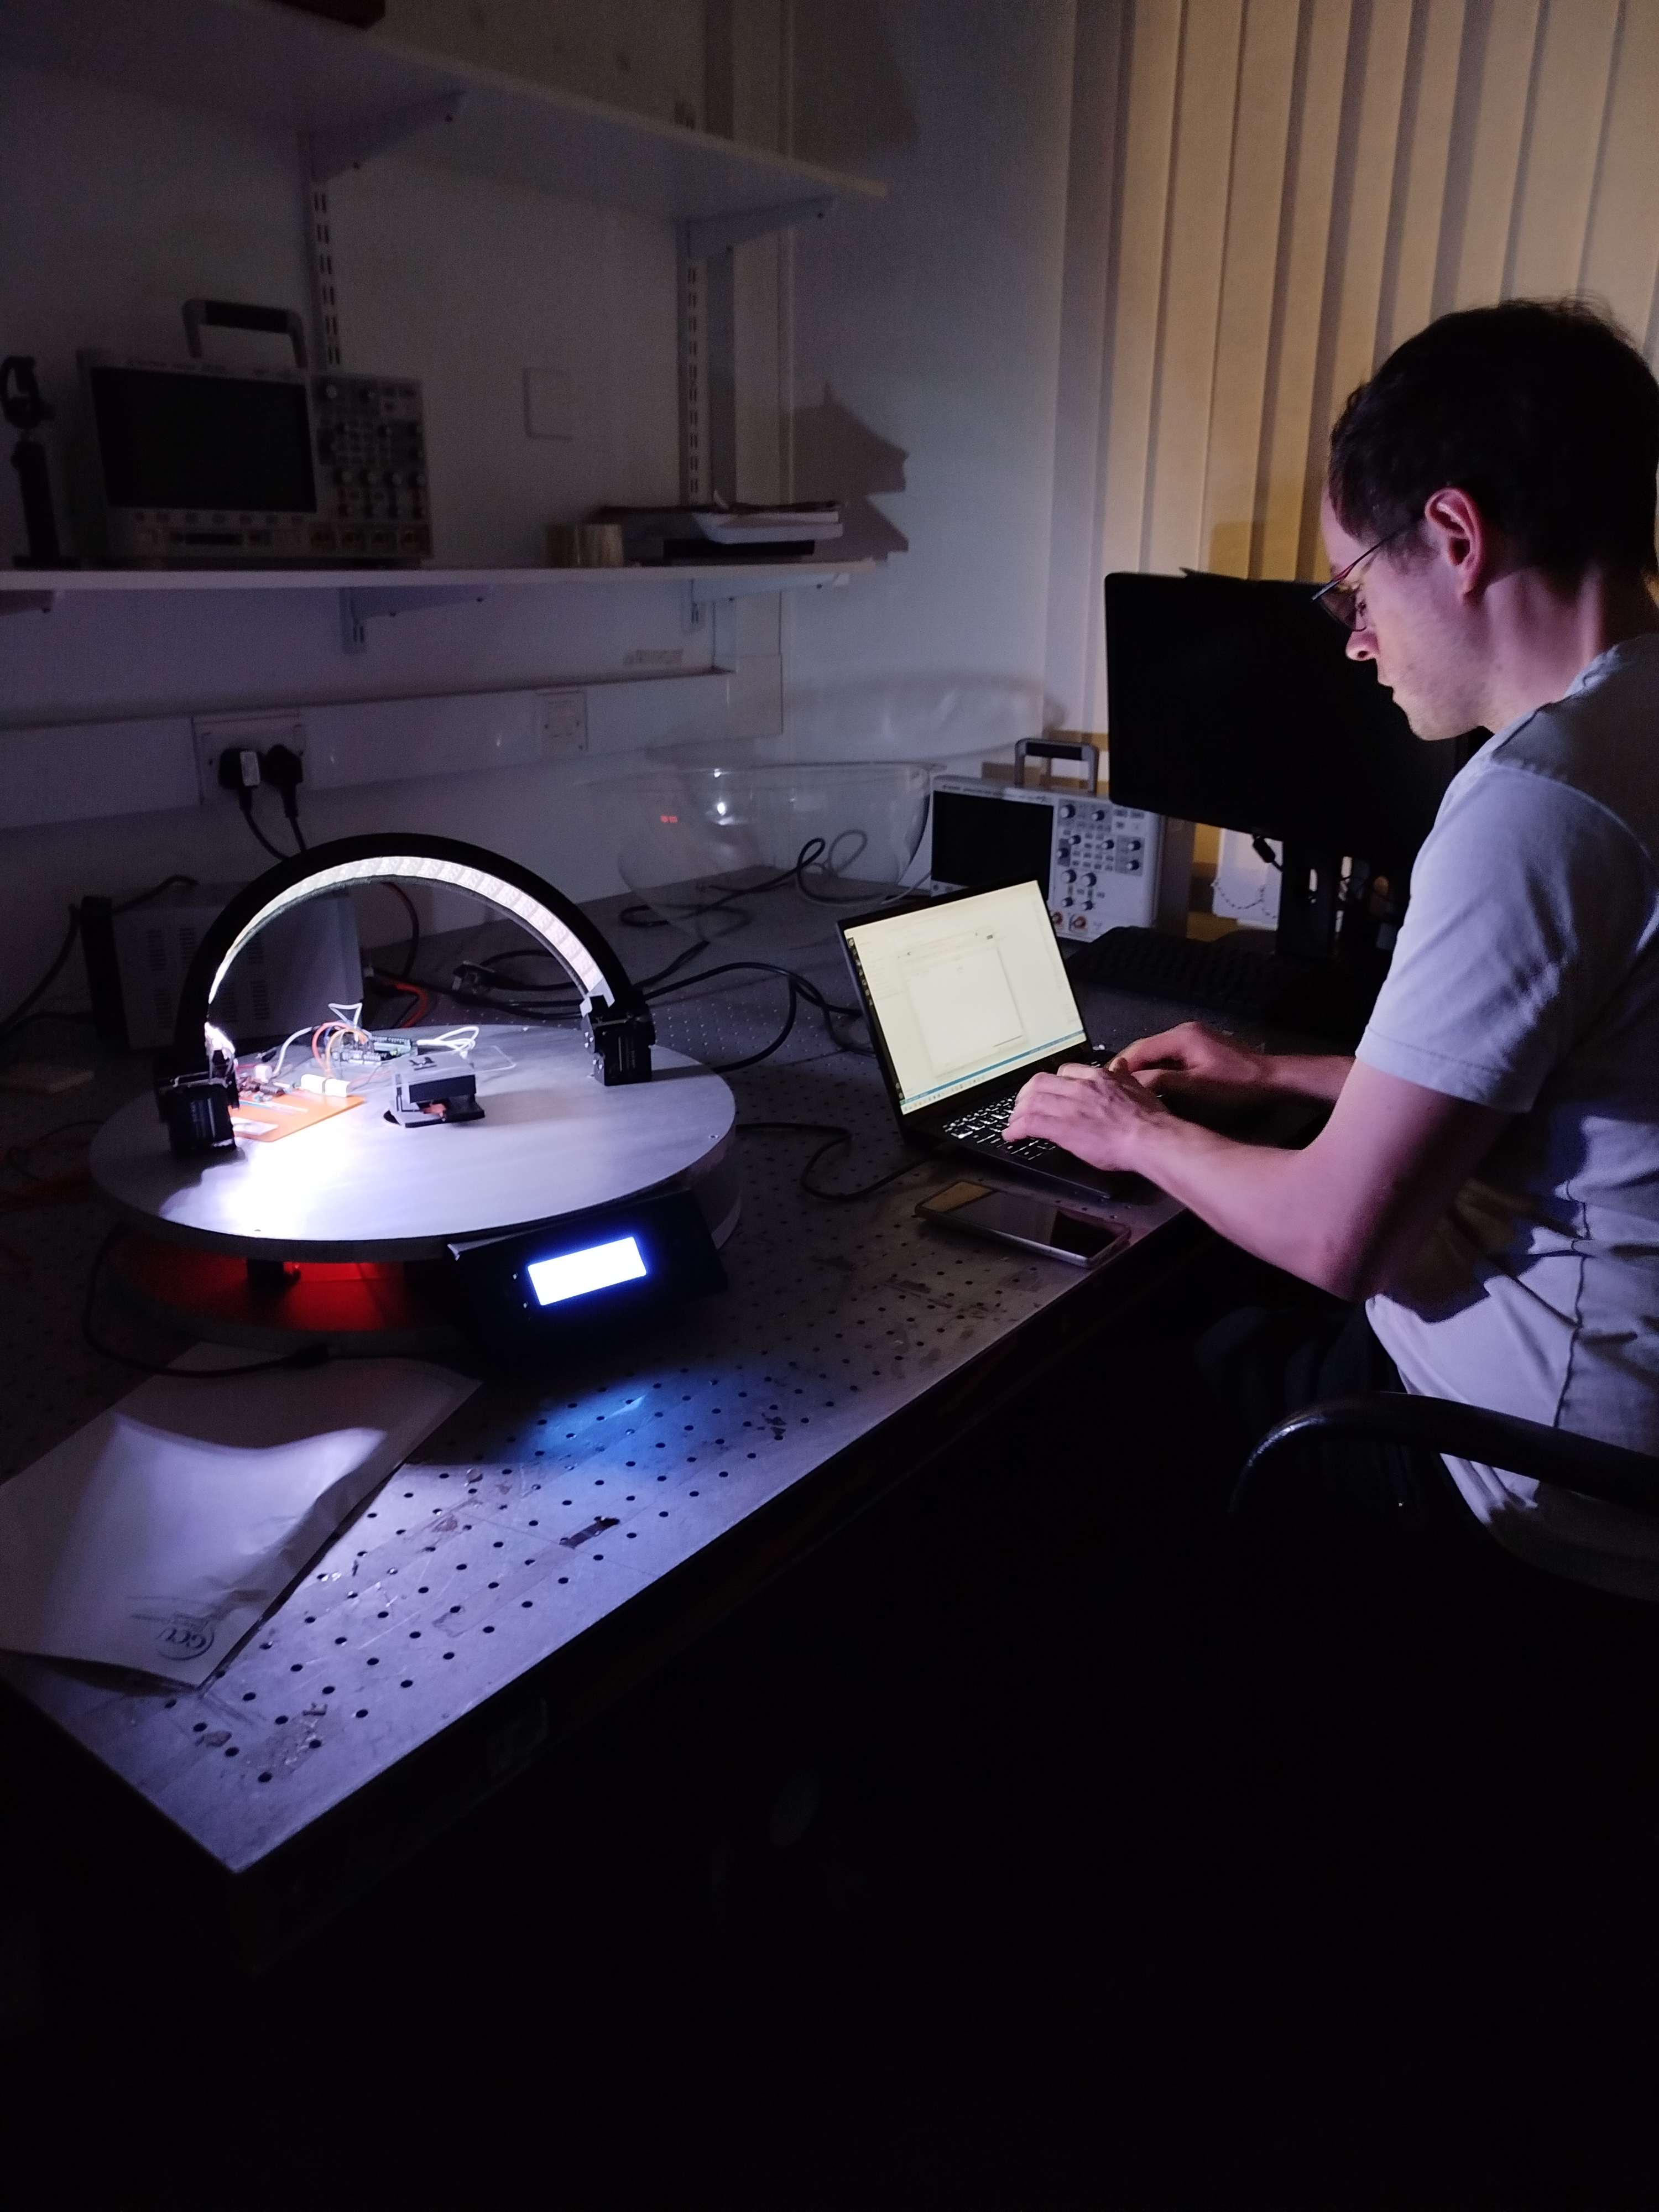
\includegraphics[width=0.7\textwidth]{figures/methodology/Prototype_testing/solarLab_test4.jpg}
     \caption*{Solar Lab Test of the Prototype 4} 
     \label{fig:Solar-Lab-Test-Prototype4}
\end{figure}

    \begin{figure}[htbp]
    \centering
    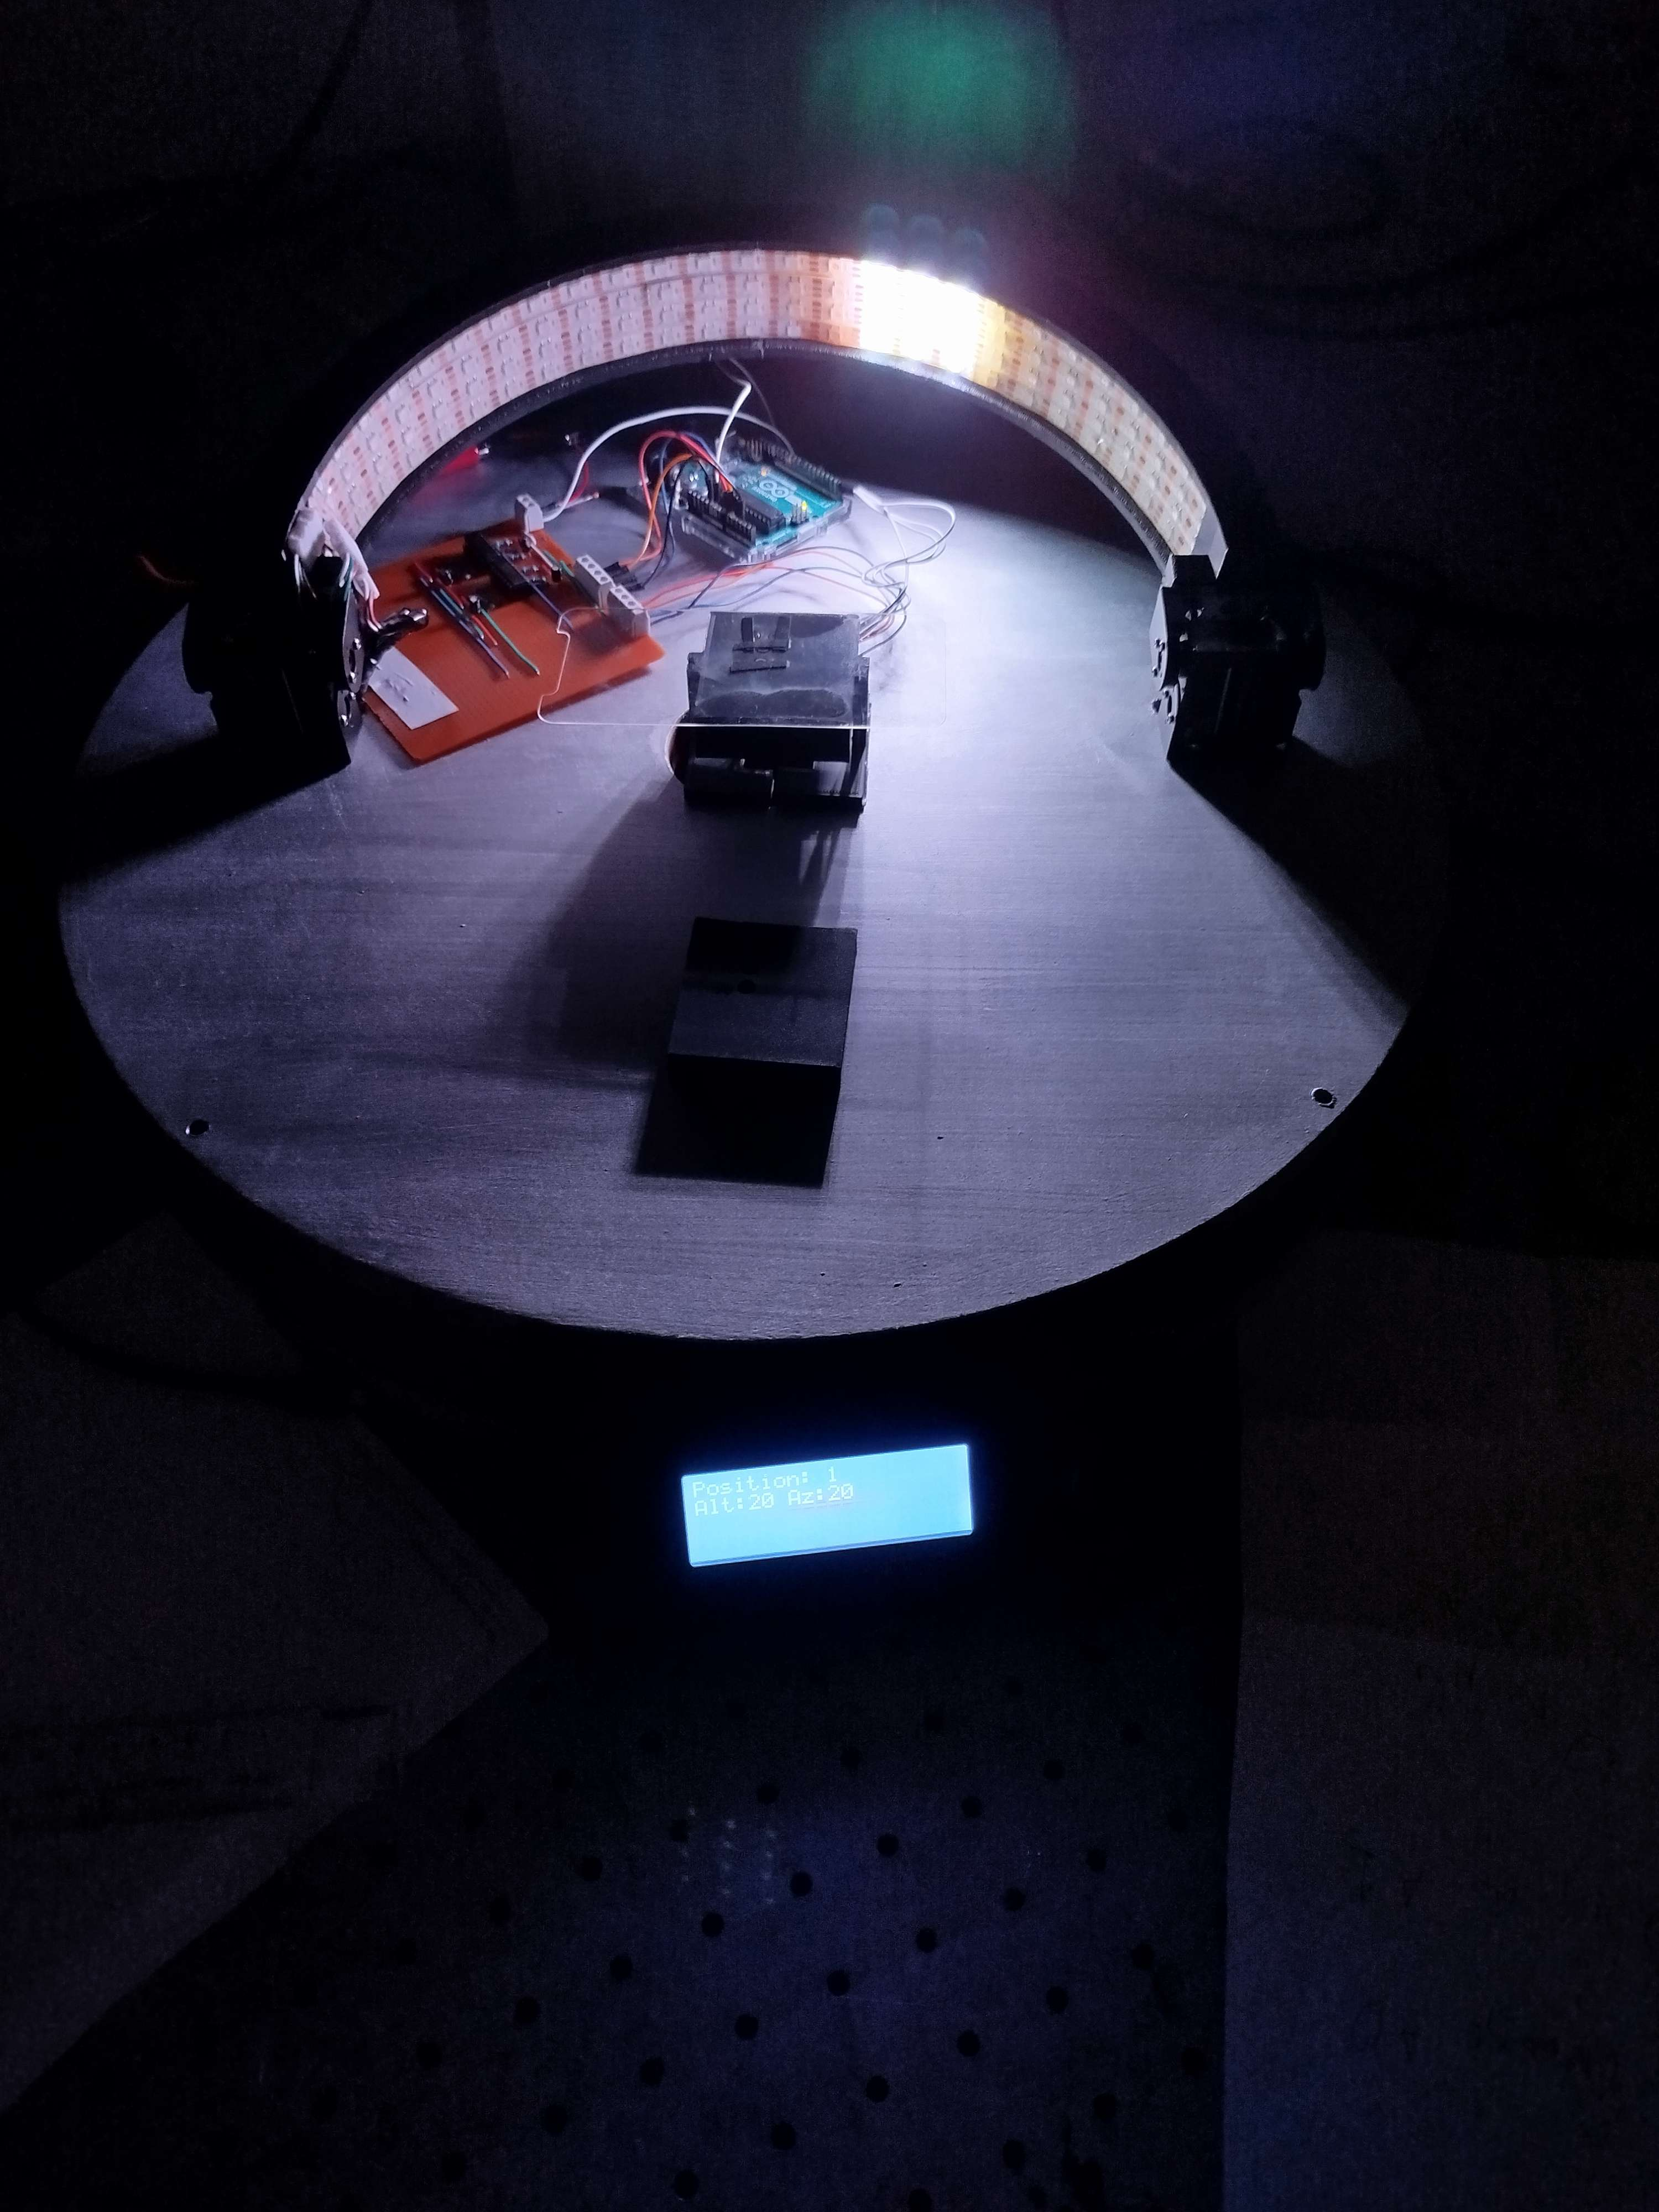
\includegraphics[width=0.7\textwidth]{figures/methodology/Prototype_testing/solarLab_test5.jpg}
    \caption*{Solar Lab Test of the Prototype 5} 
    \label{fig:Solar-Lab-Test-Prototype5}
\end{figure}
        %%%%%%%%%%%%%%%%%%%%%%%%%%%%%%%%%%%%%%%%%%%%%%%%%%%%%%%%



\end{document}